\documentclass[conference]{IEEEtran}
\IEEEoverridecommandlockouts
% The preceding line is only needed to identify funding in the first footnote. If that is unneeded, please comment it out.
\usepackage{cite}
\usepackage{amsmath,amssymb,amsfonts}
\usepackage{algorithmic}
\usepackage{graphicx}
\usepackage{textcomp}
\usepackage{kotex}
\usepackage{xcolor}
\usepackage{listings}
\usepackage{url}
\usepackage{float}
\usepackage{tabularx}
\usepackage{graphicx}
\usepackage{algorithm}
\usepackage{algpseudocode}


\def\BibTeX{{\rm B\kern-.05em{\sc i\kern-.025em b}\kern-.08em
    T\kern-.1667em\lower.7ex\hbox{E}\kern-.125emX}}

\begin{document}

\title{Stroke Striker\\}

\author{\IEEEauthorblockN{Lee Seungsu}
\IEEEauthorblockA{\textit{dept. Computer Science} \\
Korea \\
2019034702 \\
mqm0051@gmail.com}
\and
\IEEEauthorblockN{Park Geonryul}
\IEEEauthorblockA{\textit{dept. Computer Science} \\
 Korea \\
2019040564 \\
geonryul0131@gmail.com}
\and
\IEEEauthorblockN{Elia Ayoub}
\IEEEauthorblockA{\textit{dept. Computer Science} \\
France \\
9170420231 \\
elia-ayoub@outlook.com}
\and
\IEEEauthorblockN{Ryan Jabbour}
\IEEEauthorblockA{\textit{dept. Computer Science} \\
France \\
9191820235 \\
jabbourryan2@gmail.com}
}

\maketitle

% %\begin{abstract}
% With the development of technology in the world, the average life expectancy of humans is gradually increasing worldwide.
% This means that old people would have to live a healthy life for a long time.
% However, elderly people get reluctant to go to the hospital, and if they do, they get examined at the hospital only when symptoms develop even though they are more vulnerable to diseases.
% We are going to present to you a new home appliance that can actively examine one's health, advice him, and warn him about suspicious symptoms correlated to dangerous diseases while keeping a diagnostic report to the user.
% \end{abstract}

\begin{abstract}
 Stroke is an acute and severe disease worldwide ranked as the \cite{r1} fourth cause of death in South Korea and \cite{r2} the fifth cause of death in the United States of America.\\ \\ \cite{r3} The most effective time to remove the blood clots caused by this disease is within an hour of the stroke, but of course, the sooner, the better. Otherwise, treatment should be administered within at least three hours in order to minimize potential complications. Since the hospital needs to conduct an MRI and a CT scan for diagnosis, we can consider \cite{r4} the best time to arrive at the hospital after a stroke would be one hour. However, in case of the onset of prognostic symptoms, the time of stroke cannot be predicted, so it is recommended that you go to the hospital right away.\\ \\Fortunately, \cite{r5} stroke has a reliable pre-hospital diagnostic method called BE-FAST (Balance, Eyes, Face, Arm, Speech, Terrible headache). Facial expression changes caused by paralysis of facial muscles are a very obvious symptom of stroke to detect, so you can make a relatively accurate diagnosis about it.\\ \\That's where we're putting our focus.\\ \\Of course, there are currently many applications that can be used to diagnose patients using this method. But they're all "passive" applications where you should turn on the app and take pictures of yourself.\\ \\However, the importance of the software we're creating lies in the "active" part. Home appliances, typically refrigerators and TVs, are used daily by people. We know eventually that everyone opens their fridge at least once a day, even if there's no specific reason, or turn on their TV. According to a 2012 Consumer Electronics Industry Survey, a family of four opens the refrigerator on average 40 times a day and it means 10 times a day per person. Putting their attention on this stat, \cite{r6} LG Electronics not only achieved great results with the design of "Magic Space" but also significantly reduced electricity use at home. \cite{r7} In addition, Americans open their refrigerators an average of 33 times a day, according to ENERGY STAR, a program run by the U.S. Environmental Protection Agency and the U.S. Department of Energy.\\ \\Considering everything cited above, a brief intro of our project: the refrigerator would be equipped with a camera to scan the users' facial expressions when standing face to it. If a risk of stroke is detected, a speaker implemented informs the user of his condition right away.\\ \\If this health check service was supported by every home appliance, we could imagine a household that actively protects our health in real-time daily and not just a passive household that passively neglect dangerous health issues.
\end{abstract}

%\begin{IEEEkeywords}
%component, formatting, style, styling, insert
%\end{IEEEkeywords}

\begin{table}[h]
    \caption{a list of role assignment}
    \begin{tabular}{|p{2.6cm}|p{1.7cm}|p{3.4cm}|}
    \hline
    Role & Name & Task Description \\ \hline
      Development Manager & Lee Seungsu & Lee Seungsu was responsible for designing the overall concept of the software and finding the basis for various claims. He implemented real-time face landmark detection using a Raspberry Pi and subsequently extended the functionality to capture facial images and send them to an Amazon server.\\ \hline
      Software Development & Park Geonryul & Park Geonryul was in charge of the actual implementation of systems as well as machine learning. He implemented and trained various artificial intelligence models and ultimately achieved accurate stroke detection through the Amazon Rekognition model.\\ \hline
      Customer & Elia Ayoub & Elia, as a customer and user of the products and servies provided by the team, had to deliver an objective feedback on them accordingly.\\ \hline
      Project Analysis & Ryan Jabbour & Ryan was given the task of checking all the documentation to present and the logical development process of the project.\\ \hline
    \end{tabular}
    \end{table}


\section{\textbf{Introduction}}
\subsection{\textbf{Motivation}\\}
\begin{itemize}
    \item \textbf{The Problem}\\
    \\ \cite{r8} According to the National Statistical Office of the Republic of Korea, nearly 60,000 of the total 120,000 stroke patients in 2021 were not transferred to the emergency room until more than six hours after the outbreak. Fewer than 15\% of the people arrived at the emergency room in less than an hour, and half of them were patients living in the Seoul-Gyeonggi area. \cite{r9} The number of patients at risk is increasing in provinces and the medical infrastructure is insufficient, so initial diagnosis or prevention is not possible, and even if it could be, follow-up will inevitably be delayed. After all, time is the lifeblood of a stroke and every minute counts. You need to quickly notice the signs but rarely do patients check signs of stroke daily.\\ \\With the development of technology and healthcare in the world, life expectancy has gradually increased over the years and is approaching a staggering 80 years old. Health is one of the most important factors in a person's life. However, there are cases where the elderly are reluctant to go to the hospital due to their habits or due to their misunderstandings arising from their experiences. There are cases in which the right time to prevent or treat the person had already passed and it was already too late. Then, in this context, not worrying about one’s health and not taking preemptive measures can lead to serious social problems.\\ \\This problem is not only defined to the older generation. \cite{r8} According to the National Medical Center, the incidence of stroke among people in their 20s and 30s is rising every year. The stereotype that stroke is a disease only the elderly can have can often push people to neglect it even when having premonitory symptoms.\\ \\Moreover, a growing number of people have started living alone, especially in South Korea, and similar problems can appear in these single-person households. Because of living alone, ones can’t point out their unhealthy habits. And if this person gets an acute disease, they won’t be able to take the proper measures leading to serious health problems. \cite{r10} As the proportion of single-person households in Korea approaches 34.5\%, chances for them to recognize acute diseases in the early stages are also decreasing.\\ \\In order to become a better society, we must overcome all those problems. The reality is that people's recognition rate of early stroke symptoms is very low. \cite{r11} According to the Korea Centers for Disease Control and Prevention, only 54\% of all respondents were correct for early stroke symptoms. Although awareness reached a high of 61\% during the pandemic in 2019 - presumably because people cared a lot about health issues due to pandemic - it has been low since 2019.\\ \\Let's summarize everything. First, people aren't as wary or concerned about strokes as we might think. Second, when a stroke occurs, it is quite rare for patients to arrive at the hospital within the recommended time, and most of them actually live in the metropolitan area where the medical infrastructure doesn't meet quality requirements. Third, the elderly, who are at high risk of getting the disease, are concentrated in provinces with low-quality healthcare institutions, and have low awareness about the disease so it is unlikely for them to respond to premonitory symptoms. Fourth, although the incidence rate of stroke for people in their 20s and 30s is rising, their vigilance is still very low. Fifth, as the number of single-person households is increasing, ones are not able to detect stroke beforehand and initial responses are becoming insufficient.\\ \\In order for the passive detectors to be effective, people of all ages must be aware of stroke on their own and check it periodically. However, no method, from promotions to campaigns, seems to be able to enhance this phenomenon. If this was the case, \cite{r12} the prognostic indicator for stroke should have been higher.\\ \\Therefore, what we need is an active, every day, stroke checker.\\
\end{itemize}
\begin{itemize}
    \item \textbf{The Solution}\\
    \\As we said at the beginning, \cite{r7} people open their refrigerator approximately once a day. Our concept benefits from this habit. There are already many refrigerators equipped with IoT technology, so our idea is to equip our home appliances with cameras. The refrigerator detects the person's face and his landmark through computer vision when he stands in front of it.\\ \\Using BE-FAST diagnostic methods, if a specific facial expression such as paralysis of one facial muscle is detected, "Strike Stroke" will notify the user right away. The notification method would be through a push-message on your phone application (Thin-Q) or by the use of an AI speaker (NUGU).\\ \\Afterwards, it will guide you to the nearest hospital or emergency center where first aid for stroke is available. It will offer users automatic connection to 119 if they approve it.\\ \\Since fixed cameras may not respond appropriately depending on the users' physical characteristics, \cite{r13} multi-angle vision technology is applied to detect them from various angles. This creates a true daily active detector, beyond the limits of difference in home structure and physical characteristics of each user.\\
\end{itemize}
\begin{itemize}
    \item \textbf{Future Expectations}\\
    \\As the artificial intelligence field is rapidly developing and computer vision is a technology that occupies a large proportion of it, it is highly likely to detect user behavior and develop it into various medical diagnosis. If these technologies are included in each of LG Electronics' home appliances, which currently have a huge share compared to other competitors, users will be able to continue to actively detect their diseases in their homes, whether in the living room, the kitchen or even the bedroom. This will allow the home to become an active diagnostic center for individuals rather than just passive living space. If this one day becomes our reality, we expect a very big paradigm shift. \cite{r14} We think home diagnostics self care, which is developing recently, is a very important technology field, and the synergy will be great if it is combined with home appliances.\\
\end{itemize}

\subsection{\textbf{Research on Related Materials}\\}
\begin{itemize}
    \item \textbf{Project MONAI}\\
    
    \begin{figure}[htp]
    \centering
    
\includegraphics[width=4cm]{images/monai.png}
    \caption{MONAI project}
    \label{fig:monai}
    \end{figure}
    
    MONAI is an initiative started by NVIDIA and King's College London to establish an inclusive community of AI researchers to develop and exchange best practices for AI in healthcare. This collaboration has expanded to include academic and industry leaders throughout the medical field.\\ \\This project is similar to our project because it is simply analyzing MRI or CT photographs with AI, but the methods used are different.\\
    \item \textbf{BASLER}\\
    % 비전 시스템의 전반적인 솔루션을 제공한다. 하드웨어와 소프트웨어를 동시에 지원하고 머신러닝 기반으로 이미지를 판별할 수 있다. 특히, 의료 관련에 특화되어 있다. 하지만 센서와 카메라가 매우 비싸 그대로 가전에 적용하기는 어렵다.
    \\This company actually provides an overall solution for the vision system. Their products support hardware and software at the same time and can analyse images based on machine learning. However, their cameras and sensors are very expensive, so it would be difficult to apply them to home appliances as they are presented in this project.\\
    \item \textbf{Kaggle Project}\\

    \begin{figure}[htp]
    \centering
    
\includegraphics[width=3cm]{images/kaggle.png}
    \caption{Kaggle}
    \label{fig:kaggle}
    \end{figure}
    
    % kaggle에서 진행하는 뇌졸중 감지 프로젝트이다. 우리 프로젝트의 AI 모델로써 사용가능하다. 이 프로젝트의 판별 알고리즘은 2D 이미지를 기반으로 진행하기 때문에 우리 프로젝트의 3D 인식과는 다른 점이 있다.
    It is a stroke detection project undertaken by Kaggle. It can be used as an AI model for our project but since the algorithm used in this project is based on 2D images, it differs from the 3D recognition we need to use in our project.\\
    \item \textbf{Related Papers}\\
    % 우리의 프로젝트의 이론적인 근거를 찾기 위해 많은 논문을 조사했다. 조사한 결과 주요한 논문은 다음과 같다. FAST 기법으로 얼굴 사진으로 뇌졸중을 판단할 수 있고, 하나의 카메라로 multi-angle의 얼굴 표정을 검출할 수 있다. 마지막으로 CNN을 이용해 facial landmark로 딥러닝을 수행할 수 있음을 알 수 있었다.
    \\We researched numerous papers in order to study the theoretical part of our project.\\ 
    % The FAST technique can determine a stroke with a facial photo.Then, a multi-angle facial expression can be detected with one camera. Finally, we found that deep learning can be performed with facial landmark using CNN.

    1. Multi-Angle detector\cite{r15}\\
    \\This paper introduces lightweight deep network and combining key point feature positioning for multi-angle facial expression recognition. Using robot dog to recognize facial expressions will be affected by distance and angle. To solve this problem, this paper proposes a method for facial expression recognition at different distances and angles, which solved the larger distance and deflection angle of facial expression recognition accuracy and real-time issues.\\

    2. Raspberry Pi Based Emotion Recognition using OpenCV, TensorFlow, and Keras \cite{r16}\\
    \\In this tutorial, they implement an Emotion Recognition System or a Facial Expression Recognition System on a Raspberry Pi 4. The apply a pre-trained model in order to recognize the facial expression of a person from a real-time video stream. The “FER2013” dataset is used to train the model with the help of a VGG-like Convolutional Neural Network (CNN).\\

    3. Connect a Raspberry Pi or other device with AWS\cite{r17} \\
    \\This step-by-step tutorial guides through all the steps you need to take in order to connect a Raspberry Pi or any other device with AWS. It tells you how to set up the device, install the required tools and libraries for the AWS IoT Device SDK, install AWS IoT Device SDK, install and run the sample app, as well as view the messages from the sample app in the AWS IoT console.\\

    4. Realtime Facial Emotion Recognition\cite{r18} \\
    \\This repository demonstrates an end-to-end pipeline for real-time Facial emotion recognition application through full-stack development. The front-end is developed in react.js and the back-end is developed in FastAPI. The emotion prediction model is built with Tensorflow Keras, and for real-time face detection with animation on the front-end, Tensorflow.js have been used.\\

    5. Kaggle FER-2013 DataSet\cite{r19} \\
    \\The data consists of 48x48 pixel grayscale images of faces. The faces have been automatically registered so that the face is more or less centred and occupies about the same amount of space in each image.\\ \\The task is to categorize each face based on the emotion shown in the facial expression into one of seven categories (0=Angry, 1=Disgust, 2=Fear, 3=Happy, 4=Sad, 5=Surprise, 6=Neutral). The training set consists of 28,709 examples and the public test set consists of 3,589 examples.\\

    6. Facial landmarks with dlib, OpenCV, and Python\cite{r20} \\
    \\This post explains line by line a source code and demonstrates in details what are face landmarks and how to detect facial landmarks using dlib, OpenCV, and Python. Also, it introduces alternative facial landmark detectors such as ones coming from the MediaPipe library which is capable of computing a 3D face mesh.\\
\end{itemize}
\section{\textbf{Requirements}}
\subsection{\textbf{Training AI model}}
% 인공지능 모델을 데이터를 기반으로 학습시키는 과정이다. 뇌졸중 환자의 face drooping이 존재하는 이미지와 존재하지 않는 정상인의 이미지를 통해 학습한다. 이미지는 Tensor 형태로 변환되고 flatten 되는 이미지 전처리 과정을 거친다. 이떼 모델은 classification이 가능한 모델이어야 하고 SVM, Transformer 기반의 ViT, Naive bayes classifier 등이 있다.
It is a process of training an artificial intelligence model based on data. It learns through images with face drooping of stroke patients and images of normal people who do not exist. The image is converted into a Tensor form and flatten through an image preprocessing process. The model should be a classification-capable model, and includes Support Vector Machine, Visual Transformer, and Naive bayesian classifier.\\
\subsection{\textbf{Saving trained AI model}}
% 웹 서버에서 학습을 진행하기에는 어려움이 있으므로 외부에서 인공지능 모델을 다량의 데이터를 기반으로 학습하고 그 파일을 local computer에 저장한다. pickle 혹은 joblib 등을 이용할 수 있다.
Since it is difficult to train the AI model on a web server, the model should be trained from the outside based on data and the file is stored in the local computer. Pickle or joblib can be used.\\
\subsection{\textbf{Loading trained AI model}}
% 저장한 학습된 인공지능 모델을 적절한 위치에서 다시 불러올 수 있어야 한다. 불러오는 위치는 AWS Lightsail처럼 가상 머신이기 때문에 local computer에서 가상머신으로 파일을 옮기는 scp 명령어가 사용될 것이다. 
The stored trained artificial intelligence model should be able to be retrieved from the appropriate location. Because the location to import is a virtual machine, like AWS Lightsail, the 'scp' command to move files from the local computer to the virtual machine will be used.\\
\subsection{\textbf{Classifying Image with trained AI model}}
% 인공지능 모델을 학습시키는 것과 유사하게 이미지 전처리 과정이 우선이다. 전처리된 이미지를 학습된 인공지능 모델에 입력값으로 넣어 예측값을 받는다. 이때, 뇌졸중과 같은 의료 정보이므로 0 또는 1과 같이 hard-classification으로는 부족하다. 각 예측값의 확률도 같이 예측하도록 구현한다.
Similar to training an artificial intelligence model, the image preprocessing process comes first. Preprocessed image is input to the trained artificial intelligence model to receive predicted values. At this time, since it is medical information such as stroke, hard-classification such as 0 or 1 is not enough. The probability of each predicted value is also predicted.\\
\subsection{\textbf{Returning the result}}
% 인공지능이 반환한 예측값을 웹 통신으로 보낸다. 이를 위해 적합한 포맷으로 변환하는 과정을 거친다. classification된 결과와 각 결괏값에 대한 확률이 포함되어야 하고 Json format으로 변환되어 전송된다.
The predicted value returned by trained AI model is sent via web communication. For this purpose, it goes through a process of converting to an appropriate format. The classified results and the probability for each result value must be included and converted to JSON format and transmitted.\\
\subsection{\textbf{Get Image with API}}
% 웹 프레임워크의 기능을 이용해 외부에서 이미지 파일을 받는다. Post 방식으로 이미지 파일 자체가 전달되며 이는 위에서 언급한 전처리 과정을 거쳐 인공지능 모델의 인자로 전달된다.
Receive image files using the functions of the web framework. The image file itself is delivered using the Post method, and is passed as a parameter to the artificial intelligence model through the preprocessing process mentioned above.\\
\subsection{\textbf{Post the result with API}}
% 위의 Returning the result에서 Json format으로 예측값을 변환하여 만든 값을 Post 요청을 보냈던 곳으로 반환한다. 이 기능은 웹 프레임워크의 기능을 이용해 구현한다.
In 'Returning the result' part above, the predicted value is converted to JSON format and the result value is returned to the place where the Post request was sent. This function is implemented using the functions of the web framework.\\

\subsection{\textbf{Encapsulate the AI model}}
% 구현의 편의성을 위해 위에서 언급한 내용을 하나의 파일에서 하나의 함수로 모아 캡슐화한다.
For convenience of implementation, the contents mentioned above are gathered and encapsulated into one function in one file.\\
\subsection{\textbf{Run the Web Server}}
% 위의 하나의 파일을 작동시켜 웹 서버를 배포한다. 외부의 IP에게 개방해 접속이 가능케 한다.
Deploy the web server by running the above file. Opens to external IP to enable connection.\\

\subsection{\textbf{Amazone Lightsail}}

\begin{figure}[htp]
\centering

\includegraphics[width=3cm]{images/aws lightsail.png}
\caption{Amazon Lightsail}
\label{fig:aws}
\end{figure}

% 인공지능 모델의 배포와 학습을 위한 서버이다. Ubuntu 기반의 x86-64로 구성되어 있다. EC2를 사용해 가상 인스턴스를 만들었으며 탄력적 IP로 접근 가능하도록 보안 설정을 했다.
It is a server for the deployment and training of the artificial intelligence model. It is built on an Ubuntu-based x86-64 architecture. We created a virtual instance using EC2 and configured security settings to make it accessible via an Elastic IP.\\

\subsection{\textbf{Amazon Rekogniton}}

% 이미지, 비디오를 인식하는데 특화된 AWS 인공지능 서비스 중 하나이다. 데이터가 준비된다면 모델을 학습시키는데 필요한 각종 하이퍼 파라미터를 알아서 최적화시키고 배포까지 자동으로 가능하다. 즉, 데이터, 모델 훈련, 검증, 배포까지 자동화가 가능한 기능이다.
It is one of AWS artificial intelligence services specialized in recognizing images and videos. Once the data is ready, various hyper parameters needed to learn the model can be optimized and distributed automatically. In other words, it is a function that can automate data, model training, verification, and distribution.


\subsection{\textbf{Amazon Sagemaker}}
\subsubsection{\textbf{Autopilot}}

 With SageMaker Autopilot, you simply provide a tabular dataset and select the target column to predict. SageMaker Autopilot explores your data, selects the algorithms relevant to your problem type, prepares the data for model training, tests a variety of models, and selects the best performing one. You can then deploy one of the candidate models or iterate on them further to improve prediction quality.

 Since full automation is possible as above, all you have to do is prepare the input data and enter the input according to the settings.

\subsubsection{\textbf{CodePipeline}}

This is an Amazon service that supports pipelines. MLOps can be developed using this pipeline.

\subsection{\textbf{Amazon Polly}}

Amazon Polly uses deep learning technologies to synthesize natural-sounding human speech, so you can convert articles to speech. With dozens of lifelike voices across a broad set of languages, use Amazon Polly to build speech-activated applications.
We use this for translating text into voice. By using this, we can inform customers about the process and results through voice

\begin{figure}[htp]
\centering
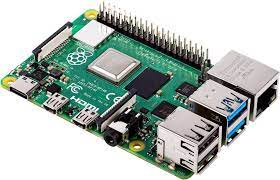
\includegraphics[width=4cm]{images/raspberrypi.jpeg}
\caption{Raspberry Pi}
\label{fig:raspberryPi}
\end{figure}

\subsection{\textbf{Raspberry Pi}}
% 사용자의 사진을 촬영하는 카메라를 통제하고 촬영한 사진을 웹서버와 통신이 가능하게 한다. 인공지능 모델이 사진을 기반으로 뇌졸중 여부를 판단한 결과를 다시 받아 다시 사용자에게 알려주는 역할을 맡았다. 이 과정은 NUGU 스피커로 청각적으로나 Dashboard를 통해 시각적으로 표현이 가능하다.
It controls a camera that captures user photos and enables communication with a web server. The artificial intelligence model is responsible for determining the presence of a stroke based on the photos and relaying the results back to the user. This process can be conveyed either audibly through NUGU speakers or visually through a dashboard. We use this to create a real IoT program.\\

\subsection{\textbf{SSH}}
To enhance coding productivity on Raspberry Pi, we use SSH. This allows us to remotely connect to the Raspberry Pi from our local desktop and use the same IDE for increased efficiency.
SSH enables the connection between the Raspberry Pi and the local desktop when they are on the same Wi-Fi network.\\

\subsection{\textbf{Camera}}
To execute our project, a camera is essential. Since we are planning to implement IoT technology using Raspberry Pi, we opted for the highly compatible camera, PiCamera2. This allows us to automatically forward the camera to camera-related functions used in OpenCV.\\

\subsection{\textbf{LED module}}
We use the LED module for privacy protection. When the device connects to the server or the internet, the LED lights up, allowing users to be aware of the current status. This is to prevent crimes resulting from hacking.\\

\subsection{\textbf{OpenCV}}

\begin{figure}[htp]
\centering

\includegraphics[width=2cm]{images/opencv.png}
\caption{OpenCV}
\label{fig:opencv}
\end{figure}

OpenCV is a powerful library widely used for computer vision and image processing tasks. It allows us to perform various operations, such as reading and saving images. Additionally, it provides the capability to perform color space transformations, which is crucial for efficiency. Resizing images is also possible, and OpenCV offers a wide range of algorithms and functions for tasks like face pattern detection. Furthermore, it allows for feature point extraction and image processing, making it a versatile tool for a variety of tasks.\\



\subsection{\textbf{Tensorflow Serving}}

\begin{figure}[htp]
\centering

\includegraphics[width=4cm]{images/tensorflow.png}
\caption{TensorFlow}
\label{fig:tensorflow}
\end{figure}

% Tensorflow를 기반으로 인공지능 모델을 개발했을 때, 배포를 간편하게 진행할 때 필요하다.
When developing an artificial intelligence model based on TensorFlow, it is necessary for streamlined deployment.\\

\subsection{\textbf{Privacy Protection}}
% 사용자의 사진을 촬영하는 카메라로서 사용되지 않는 경우에는 작동이 불가능해야 한다. 개인정보 보호를 위해 카메라가 작동 중이면 맥북의 웹캠처럼 표시를 가능하게 하거나 zoom의 기능과 같이 주변부를 흐리게 처리할 수 있다.
Privacy policy is of utmost importance in our project, given that it involves capturing a user's everyday life. We aim to ensure privacy through a two-step approach. \\
\subsubsection{\textbf{Background Blur}}
First, we will apply blurring to the background, excluding the face. \\
\subsubsection{\textbf{Two-level detection and LED module}}
Second, we will implement a real-time detection algorithm that operates locally without internet or server connectivity in normal circumstances. In the event of a detected risk of stroke, the system will establish a connection to the server, capturing an accurate photo of the user to utilize a trained artificial intelligence model. If connected to the server or the internet, an LED module located next to the camera will activate, allowing the user to visually confirm the device's status.\\

\subsection{\textbf{Speaker}}

% 인공지능 스피커로 본 프로젝트에서는 라즈베리 파이에서 전송된 뇌졸중 여부를 사용자에게 청각적으로 전달할 수 있다. 이 외에 사용자가 원할 때 촬영을 시작하도록 trigger를 인식할 수 있다.
Using a speaker gives the ability to audibly relay stroke information sent from the Raspberry Pi to the user. 

\subsection{\textbf{Dashboard}}
% 뇌졸중 여부를 시각적으로 표현해준다. 라즈베리 파이에서 전송된 뇌졸중 여부와 확률, chatGPT로 작성한 건강에 관련된 유용한 정보를 사용자에게 시각적으로 보여준다. 유용한 정보의 예시는 다음과 같다. 뇌졸중에 도움이 되는 음식이나 생활습관, 만약 발병한다면 어떻게 해야 하는지에 대한 정보가 포함된다.
It visually expresses whether you have a stroke or not. It displays stroke information and its probability sent from the Raspberry Pi, along with health-related useful information generated by ChatGPT, to the user. Examples of useful information include foods and lifestyle habits that can be beneficial in the event of a stroke, as well as guidance on what to do if a stroke occurs.\\
\subsubsection{\textbf{Probability of Stroke}}
% API를 통해 전송된 값에서 뇌졸중 여부의 확률값을 표현한다. 자동차의 속도 계기판을 모티브로 하여 사용자에게 직관적으로 확률을 전달한다.
It expresses the probability value of stroke from the value transmitted through the API. It transmits probabilities to users by using as a motif the speed dashboard of a car.\\
\subsubsection{\textbf{User's Image}}
% 사용자를 촬영한 사진을 보여준다. 이로써 사용자는 자신의 상태를 객관적으로 확인할 수 있으며 경각심을 일으킬 수 있다.
It displays the photo of the user, allowing the user to objectively assess their own condition and potentially raise awareness of their health.\\
\subsubsection{\textbf{Treatment Options}}
% 아래의 chatGPT를 통해 얻은 뇌졸중의 치료법을 보여주는 공간이다. 만약 사용자가 뇌졸중의 확률이 높을 경우에는 더욱 눈에 띄도록 표현할 수 있다.
It shows treatment options obtained using ChatGPT. If the user has a high probability of stroke, these treatment options can be highlighted in order to draw even more attention to the user.\\
\subsubsection{\textbf{Prevention and Information}}
% 아래의 chatGPT를 통해 얻은 뇌졸중의 예방법을 알려준다. 뇌졸중의 확률이 낮더라도 예방법을 사용자에게 알려주고, 만약 의심될 때는 어떻게 해야하는지 행동지침을 알린다. 이로써 능동적인 건강관리를 가능케 한다. 
It tells users how to prevent themselves of gettting a stroke obtained and this information is also obtained by using ChatGPT. Even if the probability of stroke is low, it still informs the user of preventions and informs him on the behavioral guidelines to have in suspicion of stroke. This enables daily active health care.\\

\subsection{\textbf{ChatGPT}}

\begin{figure}[htp]
\centering

\includegraphics[width=2cm]{images/chatgpt.png}
\caption{ChatGPT}
\label{fig:chatgpt}
\end{figure}

% 사용자의 뇌졸중 여부와 확률을 기반으로 유용한 정보를 생성해주는 생성형 AI이다. API를 이용해서 질문을 담아서 전송하고 답변을 다시 받아온다. 그 답변을 Dashboard 혹은 NUGU를 통해 사용자에게 알려준다. 
It is a generative AI that generates useful information based on the user's stroke status and probability. It uses API to send questions and receive answers. The answer is notified to the user through the Dashboard or the NUGU Speaker.\\
\subsubsection{\textbf{Question}}
% chatGPT에게 뇌졸중 관련으로 질문할 때 피상적인 표현으로 한다면 당장 병원에 가야한다는 정보만 얻는다. 인공지능 모델이 반환한 결괏값에서 확률을 추출하고 치료법과 예방법, 병원을 어떻게 골라야하는지를 직접적으로 물어본다. 
When asking questions related to strokes to ChatGPT, you only receive information suggesting an immediate need to go to the hospital. By extracting the probability from the results returned by the artificial intelligence model, we can inquire directly about treatment options, preventive measures, and guidance on selecting a hospital.\\
\subsubsection{\textbf{Answer}}
% 위의 질문 형식으로 chatGPT에게 질문하고 받은 대답이다. 이 대답은 Dashboard 혹은 NUGU로 전달되어 각각 시각적, 청각적인 표현으로 사용자에게 전달된다.
After using the question format above, the answer received from ChatGPT can be passed to the Dashboard or the NUGU Speaker then passed to the user in a visual or auditory representation.\\

\subsection{\textbf{Database}}
% 인공지능 모델의 정확도를 향상시키기 위해서 이미지를 보관하는 데이터베이스가 필요할 수 있다. 하지만 이는 개인정보로 민감할 수 있기에 데이터베이스 없이 프로젝트를 구현하는 것으로 진행할 수도 있다.
To enhance the accuracy of the artificial intelligence model, a database for storing images may be required. However, since this can involve sensitive personal information, the project can also be implemented without a database.\\
\section{\textbf{Development Environment}}

% \subsection{Choice of software development platform}
\subsection{\textbf{OS}}
% 우리는 리눅스의 일종인 우분투를 기본 OS로 설정했다. 이 우분투는 학습된 AI 모델이 웹 서버를 통해 배포될 때 필요한 가상 머신의 OS이다. CLI 기반으로 가볍고 빠르며 프로그래머 입장에서 친숙한 운영체제이기 때문에 우분투를 선택했다.
We set Ubuntu, a type of Linux, as the default OS. This Ubuntu is the OS of the virtual machine required when the learned AI model is deployed through a web server. I chose Ubuntu because it is a CLI-based, lightweight, fast, and familiar operating system for programmers.\\
\subsection{\textbf{Raspberry Pi}}
%우리의 목적은 가전기기에 인공지능을 탑재해 스마트 IoT를 만드는 것이다. 따라서 진정한 IoT의 구현을 위해 Raspberry pi를 사용할 것이다. 독립적인 컴퓨터를 사용하여 가전을 통제한다는 점에서 진정한 IoT기술을 구현하고자 하였다. 데스크탑에서 우리가 의도한 프로그램을 만들어낼 수 있겠지만, 데스크탑과 가전에 들어가는 보드의 성능차이가 굉장히 많이 나기에 이것이 IoT를 위한 프로그램이라고 할 수 없다고 생각하였다. 실제로 우리의 예상대로 데스크탑에서 돌아갔던 프로그램이 라즈베리파이에서는 돌아가지 않음을 발견하였다. 대표적인 이유로 사용하는 bit나 linux version 등의 OS의 차이, default library의 차이, 카메라를 인식하는 매커니즘의 차이, CPU, GPU 등 하드웨어적 성능 차이, 발열 문제, 성능 최적화 등이 있었다. 데스크탑에서 프로그래밍을 할 때에는 잘 고려하지 않았던 부분들을 Raspberry pi를 사용함으로써 깨달을 수 있었고 이를 통해 진정한 가전을 위한 프로그램을 만들 수 있었다. Raspberry pi에서의 프로그래밍을 위해 SSH를 이용하였다. Mac OS에서 SSH를 통해 Raspberry pi에 접근하였고 코드를 썼다.SSH를 이용한 이유는 편리함 때문이다. Raspberry pi에서 직접 코딩을 하게 되면 Editor를 따로 설치해야하고 편리한 코딩을 위한 Library도 따로 설치해야한다. 또한 키보드 입력에 대한 반응속도도 빠르지 못하여 편리하지 않다. 그래서 같은 Wi-fi에 접속한 후 지정된 IP를 통해 ssh 서버를 사용하였다.%
Our goal is to integrate artificial intelligence into home appliances to create a smart IoT system. To achieve true IoT implementation, we have chosen to use Raspberry Pi. We aim to implement genuine IoT technology by controlling home appliances with an independent computer. While we can develop the intended program on a desktop, we believe it's not suitable for IoT because of the significant differences in performance between a desktop and the board used in home appliances.\\

In practice, we found that a program that worked well on a desktop did not run smoothly on a Raspberry Pi due to several factors. These factors include differences in the operating system, such as bit and Linux version, variations in default libraries, differences in the camera recognition mechanism, variations in hardware performance, such as CPU and GPU, heat-related issues, and performance optimization. By using Raspberry Pi, we have come to realize aspects that were not carefully considered during desktop programming, allowing us to create a program truly suited for home appliances.\\

To program on Raspberry Pi, we utilized SSH. We accessed the Raspberry Pi via SSH from Mac OS and wrote the code. The reason for using SSH was convenience. Programming directly on Raspberry Pi would require installing a separate editor and libraries for efficient coding. Additionally, the response time for keyboard input is not very fast, making it less convenient. Therefore, we connected to the same Wi-Fi network and used the SSH server via the designated IP address.\\

\subsection{\textbf{Languages}}
\subsubsection{\textbf{Python}}

\begin{figure}[htp]
\centering

\includegraphics[width=3cm]{images/python.png}
\caption{Python}
\label{fig:python}
\end{figure}
    
% AI model을 설계할 때 사용한 언어이고 프로그래밍 할 때 주로 사용된 언어이다. Python으로 AI model을 만든 이유는 다음과 같다. 첫째, 다양한 라이브러리. 각종 AI model을 설계할 때 유용한 라이브러리를 python을 통해 편하게 사용할 수 있다. 예를 들면, support vector machine과 같은 기계학습 모델을 구현할 때 사용 가능한 scikit-learn, 각종 수치계산을 도와주는 numpy 등 여러 라이브러리가 준비되어 있다. 둘째, 딥러닝 프레임워크를 쉽게 사용할 수 있다. PyTorch, Keras와 같은 딥러닝을 구현하는데 도움을 주는 프레임워크를 사용하면 각 단계를 모듈화하고 특히 back-propagation을 쉽게 처리할 수 있다. 마지막으로 웹 서버와 통신하는데 필요한 API에서 FastAPI를 함께 사용해 pythonic한 코드를 만들 수 있다. 이와 같은 이유로 Python을 AI model을 구현하는데 주 언어로 사용했다.
It is the language used to design AI models and is mainly used for programming. The reasons for creating an AI model in Python are as follows.
\\

\\
First, various libraries. When designing various AI models, you can conveniently use useful libraries through Python. For example, there are several libraries available, such as scikit-learn that can be used when implementing machine learning models such as support vector machine, and numpy, which helps with various numerical calculations. \\

\\
Second, deep learning frameworks are easy to use. By using frameworks that help implement deep learning, such as PyTorch or Keras, you can modularize each step and handle back-propagation especially easily. Lastly, you can create pythonic code by using FastAPI in the API required to communicate with the web server. For this reason, Python was used as the main language to implement the AI model.\\




\begin{table}[h]
    \caption{a version of Software/Language/Tool}
    \begin{tabular}{|p{2.6cm}|p{1.7cm}|p{3.4cm}|}
    \hline
    Name & Version \\ \hline
      Raspberry Pi & Raspi 4B 4GB \\ \hline
      Rasbian & Devian BookWorm \\ \hline
      Camera & PiCamera 2\\ \hline
      Ubuntu & 22.04\\ \hline
      Uvicorn & 0.23.2 with CPython 3.10.12 on Linux\\ \hline
      Python & 3.10.12 \\ \hline
      OpenCV & 4.5.5 \\ \hline
      Dlib & 19.23.2 \\ \hline
      NUGU & SKT Jan. 18 Release \\ \hline
      
    \end{tabular}
    \end{table}


\subsection{\textbf{Environment Resources}}
\subsubsection{\textbf{AWS Lightsail}}
\begin{itemize}
    \item OS: Ubuntu 22.04.1 LTS (GNU/Linux 6.2.0-1014-aws x86\_64)
    \item CPU: Intel(R) Xeon(R) Platinum 8259CL CPU @ 2.50GHz
    \item RAM: 1GB RAM
    \item Storage: 40GB SSD
\end{itemize}
\subsubsection{\textbf{Google Colab Pro}}
\begin{itemize}
    \item GPU: T4 GPU
    \item GPU RAM: 15GB
    \item System RAM: 12GB
\end{itemize}

\subsection{\textbf{Estimated Costs}}
\begin{itemize}
    \item AWS Lightsail: \$3.5/month
    \item Colab Pro: \$9.99/month
    \item Raspberry Pi 4B 4GB: \$70\\
\end{itemize}
% Google Colab Pro는 AI model 학습 시에만 사용하므로 정기적인 비용이 부과되지는 않을 것으로 사료된다. 따라서 AWS Lightsail 비용만 생각하면 된다.


\section{\textbf{Software in use}}
\subsection{\textbf{AWS}}
% Amazon Web Service로 서버를 구축하는 등의 작업을 진행했고 아래와 같은 기능을 사용했다. 
We carried out tasks such as building a server with Amazon Web Service and used the functions below. \\
\subsubsection{\textbf{AWS Lightsail}}
% AWS Lightsail로 웹 서버를 동작시킬 수 있는 가상환경을 구축했다. AWS에서 가상환경을 설정하려면 EC2도 사용할 수 있지만 AWS Lightsail을 이용한 이유는 다음과 같다. 첫째, 소규모의 프로젝트이다. EC2보다 간소화된 버전으로 비교적 제약점이 존재하지만 웹 서버로 동작시키기에는 부족함이 없고 오히려 사용하지 않는 기능들이 많은 것보다 안정적이고 단순하다. 둘째, 월정액 과금 시스템이다. EC2는 인스턴스를 사용한만큼 요금이 부과되는 방식이지만 Lightsail은 정해진 요금으로 동작하기 때문에 24시간 켜놓는 서버용 가상머신으로는 Lightsail이 더욱 적합하다고 판단했다. 위와 같은 이유로 AI model을 배포하는데 사용되는 가상머신은 AWS의 Lightsail을 사용했다. 
We built a virtual environment to run a web server using AWS Lightsail. To set up a virtual environment in AWS, you can also use EC2, but the reasons for using AWS Lightsail are as follows.\\
First, it is a small-scale project. It is a simpler version than EC2 and has relatively limitations, but it is sufficient to operate as a web server and is more stable and simple than those with many unused functions.\\
Second, it is a monthly billing system. EC2 charges for the amount of instances used, but Lightsail operates at a fixed rate, so we decided that Lightsail would be more suitable as a server virtual machine that is turned on 24 hours a day. For the above reasons, the virtual machine used to deploy the AI model used AWS's Lightsail.\\

\subsubsection{\textbf{Amazon Rekognition}}
Amazon Rekognition removes the complexity of building visual recognition capabilities by making powerful and accurate analysis available with easy to use APIs.

Use Amazon Rekognition Custom Labels to quickly build your own custom ML model to detect objects and scenes unique to your business, simply by bringing your own training data. Leverage a guided experience, no machine learning experience is required.

Amazon Rekognition is designed to work seamlessly with other AWS services. Rekognition integrates directly with Amazon S3 and AWS Lambda so you can build scalable, affordable, and reliable visual analysis applications. You can start analyzing images and videos stored in Amazon S3 without moving any data. You can also run real-time video analysis on streams coming from Amazon Kinesis Video Streams.\\

\subsubsection{\textbf{Amazon Sagemaker}}
Amazon SageMaker is a fully managed machine learning service. With SageMaker, data scientists and developers can quickly and easily build and train machine learning models, and then directly deploy them into a production-ready hosted environment. It provides an integrated Jupyter authoring notebook instance for easy access to your data sources for exploration and analysis, so you don't have to manage servers. It also provides common machine learning algorithms that are optimized to run efficiently against extremely large data in a distributed environment. With native support for bring-your-own-algorithms and frameworks, SageMaker offers flexible distributed training options that adjust to your specific workflows. Deploy a model into a secure and scalable environment by launching it with a few clicks from SageMaker Studio or the SageMaker console. \\

\subsubsection{\textbf{AWS CodePipeline}}
AWS CodePipeline is a continuous integration and continuous delivery service for fast and reliable application and infrastructure updates.

A pipeline defines your release process workflow, and describes how a new code change progresses through your release process. A pipeline comprises a series of stages (e.g., build, test, and deploy), which act as logical divisions in your workflow. Each stage is made up of a sequence of actions, which are tasks such as building code or deploying to test environments. AWS CodePipeline provides you with a graphical user interface to create, configure, and manage your pipeline and its various stages and actions, allowing you to easily visualize and model your release process workflow.

We can use this Pipeline to achieve MLOps with our projects\\

\subsubsection{\textbf{Amazone Polly}}
Amazon Polly is a cloud service by Amazon Web Services, that converts text into spoken audio. It allows developers to create speech-enabled applications and products. Now it includes 60 voices across 29 languages, some of which are Neural Text-to-Speech voices of higher quality.


\subsection{\textbf{scp}}
scp stands for "Secure Copy Protocol," and it is a command-line tool used to securely transfer files and directories between a local host and a remote host or between two remote hosts over a network. scp is a part of the SSH (Secure Shell) suite of network protocols and provides a secure way to copy files and data from one location to another.\\
\subsection{\textbf{joblib}}
joblib is a Python library used for serialization, especially for efficiently storing and loading Python objects, often used for handling large Numpy arrays or complex data structures. It is commonly employed in data analysis, machine learning, and scientific research to save and load Python objects or share objects between processes. There are many advantages: \\
First, Efficient Serialization. joblib can serialize Python objects into binary format and store them on disk efficiently. This is particularly useful for handling large data.
\\Second, Numpy Array Support. joblib supports a variety of Python data structures, including Numpy arrays, and it can compress and store them. We use 'joblib' as below usage. Storing trained models and their parameters to reuse them later or for model deployment. \\

\subsection{\textbf{scikit-learn}}
\cite{scikit-learn}
scikit-learn (formerly scikits.learn and also known as sklearn) is a free software machine learning library for the Python programming language. It features various classification, regression and clustering algorithms including support-vector machines, random forests, gradient boosting, k-means and DBSCAN, and is designed to interoperate with the Python numerical and scientific libraries NumPy and SciPy. Scikit-learn is a NumFOCUS fiscally sponsored project.\\
\subsubsection{\textbf{skimage.io}}
scikit-image (a.k.a. skimage) is a collection of algorithms for image processing and computer vision.
The main package of skimage only provides a few utilities for converting between image data types; for most features, you need to import one of the following subpackages:\\
\subsection{\textbf{PIL}}
\cite{PIL}
Python Imaging Library is a free and open-source additional library for the Python programming language that adds support for opening, manipulating, and saving many different image file formats. It is available for Windows, Mac OS X and Linux. The latest version of PIL is 1.1.7, was released in September 2009 and supports Python 1.5.2–2.7. Development of the original project, known as PIL, was discontinued in 2011.\\
Subsequently, a successor project named Pillow forked the PIL repository and added Python 3.x support This fork has been adopted as a replacement for the original PIL in Linux distributions including Debian[5] and Ubuntu (since 13.04).\\
\subsection{\textbf{NumPy}}
\cite{NumPy}
NumPy is a library for the Python programming language, adding support for large, multi-dimensional arrays and matrices, along with a large collection of high-level mathematical functions to operate on these arrays. The predecessor of NumPy, Numeric, was originally created by Jim Hugunin with contributions from several other developers.\\

\\Python bindings of the widely used computer vision library OpenCV utilize NumPy arrays to store and operate on data. Since images with multiple channels are simply represented as three-dimensional arrays, indexing, slicing or masking with other arrays are very efficient ways to access specific pixels of an image. The NumPy array as universal data structure in OpenCV for images, extracted feature points, filter kernels and many more vastly simplifies the programming workflow and debugging.\\


\subsection{\textbf{Google Colab Pro}}
% Google Colab은 Google에서 제공하는 클라우드 기반의 Jupyter 노트북 환경이다. 이 무료 서비스를 사용하면 웹 브라우저를 통해 Python 코드를 작성하고 실행할 수 있고, 데이터 분석, 머신러닝 모델 개발, 연구 등 다양한 작업에 활용할 수 있다. 이 Google Colab을 활용하면 개인 사용자 컴퓨터의 성능과 용량 제한에 구애받지 않을 수 있고 AI model 학습을 독립적으로 진행할 수 있다. 또한 GPU나 TPU를 원격으로 연결해 사용할 수 있는 환경을 제공하기 때문에 딥러닝 모델 학습고 같은 계산 집약적인 연산에 유용하다. 마지막으로 개인 사용자 컴퓨터에서 Python code를 작성하기 위해서는 가상환경 설치 및 각종 라이브러리를 설치해야 하는 수고가 있다. Google Colab으로 사용자는 이런 수고로움에서 벗어나 온전히 구현에만 집중할 수 있다.
Google Colab is a cloud-based Jupyter notebook environment provided by Google. This free service allows you to write and run Python code through a web browser, and can be used for a variety of tasks, including data analysis, machine learning model development, and research.
\\

\\
By utilizing this Google Colab, you are not restricted by the performance and capacity limitations of individual users' computers and can proceed with AI model learning independently. In addition, it provides an environment where GPU or TPU can be remotely connected and used, so it is useful for computationally intensive operations such as deep learning model training. Lastly, in order to write Python code on a personal user computer, there is the need to install a virtual environment and various libraries. With Google Colab, users can free themselves from this hassle and focus entirely on implementation.\\

\subsection{\textbf{FastAPI}}
% FastAPI는 Python을 사용하여 빠르고 현대적인 웹 애플리케이션 및 API를 빌드하기 위한 웹 프레임워크이다. FastAPI는 사용하기 쉽고 성능이 우수하며, Python 3.6 이상 버전을 지원한다. 웹 서버를 구축할 때 FastAPI를 선택한 이유는 다음과 같다. 첫째, Python Framework. FastAPI는 Python Web Framework로 AI model을 제작할 때 사용한 언어인 Python과 연관이 깊다. 따라서 웹 서버를 제작할 때 일관성을 유지해 버그를 줄일 수 있다. 둘째, 대화형 API 문서를 생성할 수 있다. 대화형 API 문서를 통해 AI model을 만드는 개발자에서도 자체적으로 디버깅을 진행할 수 있어 편하다. 이런 이유로 FastAPI를 선택했다.
FastAPI is a web framework for building fast, modern web applications and APIs using Python. FastAPI is easy to use, has excellent performance, and supports Python 3.6 or higher. The reasons for choosing FastAPI when building a web server are as follows. 
\\

\\
First, the Python Framework. FastAPI is closely related to Python, the language used to create AI models with the Python Web Framework. Therefore, bugs can be reduced by maintaining consistency when creating a web server.
\\

\\
Second, you can create interactive API documentation. It is convenient because developers who create AI models can also carry out debugging on their own through interactive API documents. For this reason, I chose FastAPI.\\
\subsubsection{\textbf{File}}
The File class in FastAPI is used to represent an uploaded file in your application. It's commonly used as a parameter in your route's function to handle file uploads. Here is an example python code:
\begin{verbatim}
from fastapi import FastAPI, File

app = FastAPI()

@app.post("/uploadfile/")
async def upload_file(file: UploadFile):
    # Do something with the uploaded file
    return {"filename": file.filename}
\end{verbatim}
\textbf{Attributes of 'File'}
\begin{itemize}
    \item filename: This attribute contains the name of the uploaded file.
    \item content\_type: The MIME content type of the uploaded file.
    \item file: The actual file data, which can be read or processed.
\end{itemize}
\textbf{Handling the Uploaded file}
You can perform various operations on the uploaded file using the attributes. For example, you can save the file to disk, read its contents, check the content type, or perform any other custom logic.

\subsubsection{\textbf{UploadFile}}
The UploadFile class is a specialized class provided by FastAPI for handling file uploads. It contains additional functionality for managing the uploaded files. Here is an example python code:
\begin{verbatim}
from fastapi import FastAPI, UploadFile

app = FastAPI()

@app.post("/uploadfile/")
async def upload_file(file: UploadFile):
    # Do something with the uploaded file
    return {"filename": file.filename}
\end{verbatim}
\textbf{Attributes of 'UploadFile'}
\begin{itemize}
    \item filename: This attribute contains the name of the uploaded file.
    \item content\_type: The MIME content type of the uploaded file.
    \item file: The actual file data, which can be read or processed.
    \item read(): Allows you to read the content of the uploaded file as bytes.
    \item save(): You can use this method to save the uploaded file to a specified location on your server.
\end{itemize}
\\
\subsection{\textbf{Uvicorn}}
Uvicorn is a popular ASGI (Asynchronous Server Gateway Interface) server that is commonly used to deploy web applications, particularly FastAPI applications, in the Python ecosystem. It's designed for high-performance, asynchronous web serving, and it's often used in conjunction with ASGI frameworks like FastAPI and Starlette.


\subsection{\textbf{Deep learning Framework}}
% AI model을 구현할 때 딥러닝 모델을 만든다면 scikit-learn 라이브러리로는 부족하다. 각종 layer를 모듈화하고 back-propagation을 용이하게 만들어주는 딥러닝 프레임워크가 필요하다. 본 프로젝트에서는 아래와 같은 Pytorch를 사용했다.
When implementing an AI model, if you create a deep learning model, the scikit-learn library is not enough. A deep learning framework that modularizes various layers and facilitates back-propagation is needed. In this project, Pytorch was used as shown below.\\
\subsubsection{\textbf{Pytorch}}
% PyTorch는 딥러닝 및 기계 학습을 위한 오픈 소스 머신러닝 라이브러리로, 주로 Python 언어를 사용하여 모델을 개발하고 학습시키는 데 사용됩니다. PyTorch는 많은 연구원과 기업에서 널리 사용된다. 여러 Deep Learning Framework 중 Pytorch를 이용한 이유는 다음과 같다. 첫째, 동적 계산 그래프. PyTorch의 가장 큰 특징 중 하나는 동적 계산 그래프를 사용하는 것입니다. 이것은 모델을 정의하고 계산할 때 그래프를 구성하는 방식을 의미합니다. 이로써 모델을 동적으로 변경하고 디버깅하기가 훨씬 쉬워집니다. 둘째, GPU를 이용한 AI model 학습. scikit-learn을 이용해 기계학습 모델을 구현했을 때는 CPU만으로 학습을 진행했다. PyTorch는 NVIDIA GPU를 사용하여 모델 학습 및 추론을 가속화할 수 있는 기능을 제공하므로 더 빠른 학습이 가능하다. 셋째, 자동 미분이 가능하다. PyTorch는 자동 미분(automatic differentiation)을 지원하여 그래디언트(gradient)를 쉽게 계산할 수 있습니다. 이는 역전파(backpropagation) 및 경사 하강법(gradient descent)과 같은 학습 알고리즘을 구현할 때 쉽게 구현할 수 있도록 도와준다. 실제로 후술할 Transformer 알고리즘을 구현할 때 위와 같은 강점이 있는 Pytorch로 구현을 진행했다.
PyTorch is an open source machine learning library for deep learning and machine learning, primarily used to develop and train models using the Python language. PyTorch is widely used by many researchers and companies. The reasons for using Pytorch among various Deep Learning Frameworks are as follows.
\\

First, the dynamic computation graph. One of the best features of PyTorch is its use of dynamic computation graphs. This refers to the way the graph is constructed when defining and calculating models. This makes it much easier to dynamically change and debug models.
\\

Second, AI model learning using GPU. When implementing a machine learning model using scikit-learn, learning was performed using only the CPU. PyTorch provides the ability to accelerate model training and inference using NVIDIA GPUs, enabling faster training. 
\\

Third, automatic differentiation is possible. PyTorch supports automatic differentiation, making it easy to calculate gradients. This makes it easier to implement learning algorithms such as back-propagation and gradient descent. In fact, when implementing the Transformer algorithm, which will be described later, it was implemented using Pytorch, which has the above strengths.\\

\subsection{\textbf{Support Vector Machine}}
\cite{SVM}
Classifying data is a common task in machine learning.

Suppose some given data points each belong to one of two classes, and the goal is to decide which class a ''new'' data point will be in. In the case of support vector machines, a data point is viewed as a \(p\) - dimensional vector (a list of \(p\) numbers), and we want to know whether we can separate such points with a \((p-1)\)-dimensional hyperplane. This is called a linear classifier. There are many hyperplanes that might classify the data. One reasonable choice as the best hyperplane is the one that represents the largest separation, or margin, between the two classes. So we choose the hyperplane so that the distance from it to the nearest data point on each side is maximized. If such a hyperplane exists, it is known as the 'maximum-margin hyperplane' and the linear classifier it defines is known as a 'margin classifier'; or equivalently, the perceptron of optimal stability.
\\

More formally, a support vector machine constructs a hyperplane or set of hyperplanes in a high or infinite-dimensional space, which can be used for classification, regression, or other tasks like outliers detection. Intuitively, a good separation is achieved by the hyperplane that has the largest distance to the nearest training-data point of any class (so-called functional margin), since in general the larger the margin, the lower the generalization error of the classifier. A lower generalization error means that the implementer is less likely to experience overfitting.
\\

Whereas the original problem may be stated in a finite-dimensional space, it often happens that the sets to discriminate are not linearly separable in that space. For this reason, it was proposed that the original finite-dimensional space be mapped into a much higher-dimensional space, presumably making the separation easier in that space. To keep the computational load reasonable, the mappings used by SVM schemes are designed to ensure that dot products of pairs of input data vectors may be computed easily in terms of the variables in the original space, by defining them in terms of a kernel function \(k(x, y)\) selected to suit the problem. The hyperplanes in the higher-dimensional space are defined as the set of points whose dot product with a vector in that space is constant, where such a set of vectors is an orthogonal (and thus minimal) set of vectors that defines a hyperplane. The vectors defining the hyperplanes can be chosen to be linear combinations with parameters \(\alpha_i\) of images of feature vectors \(x_i\) that occur in the data base. With this choice of a hyperplane, the points \(x\) in the feature space that are mapped into the hyperplane are defined by the relation \(\textstyle\sum_i \alpha_i k(x_i, x) = \textbf{constant}.\)  Note that if  \(k(x, y)\) becomes small as \(y\) grows further away from \(x\), each term in the sum measures the degree of closeness of the test point \(x\) to the corresponding data base point \(x_i\). In this way, the sum of kernels above can be used to measure the relative nearness of each test point to the data points originating in one or the other of the sets to be discriminated. Note the fact that the set of points \(x\) mapped into any hyperplane can be quite convoluted as a result, allowing much more complex discrimination between sets that are not convex at all in the original space.
\\


\subsubsection{\textbf{Non-linear kernel}}
We use rbf kernel to deal with non-linear problem. These are introduction about kernel method. The algorithm is formally similar, except that every dot product is replaced by a nonlinear kernel function. This allows the algorithm to fit the maximum-margin hyperplane in a transformed feature space. The transformation may be nonlinear and the transformed space high-dimensional; although the classifier is a hyperplane in the transformed feature space, it may be nonlinear in the original input space.
\\

It is noteworthy that working in a higher-dimensional feature space increases the generalization error of support vector machines, although given enough samples the algorithm still performs well.\\

Some common kernels include: \\
* Polynomial (homogeneous):

\[k(\mathbf{x}_i, \mathbf{x}_j) = (\mathbf{x}_i \cdot \mathbf{x}_j)^d\]
Particularly, when \(d=1\), this becomes the linear kernel. \\

* Polynomial(inhomogeneous):

\[k(\mathbf{x}_i, \mathbf{x}_j) = (\mathbf{x}_i \cdot \mathbf{x}_j + r)^d\]

* Gaussian radial basis function:

\[k(\mathbf{x}_i, \mathbf{x}_j) = \exp\left(-\gamma \left\|\mathbf{x}_i - \mathbf{x}_j\right\|^2\right)\]

for \(\gamma > 0\). Sometimes parametrized using \(\gamma = 1/(2\sigma^2)\). \\

* Sigmoid function (Hyperbolic tangent):

\[k(\mathbf{x_i}, \mathbf{x_j}) = \tanh(\kappa \mathbf{x}_i \cdot \mathbf{x}_j + c)\]
for some (not every) \(\kappa > 0\) and \(c < 0\) \\


% \subsubsection{\textbf{Computing the SVM classifier}}
% Computing the (soft-margin) SVM classifier amounts to minimizing an expression of the form
% \[\left[\frac 1 n \sum_{i=1}^n \max\left(0, 1 - y_i(\mathbf{w}^\mathsf{T} \mathbf{x}_i - b)\right) \right] + \lambda \|\mathbf{w}\|^2\].
% \\

% We focus on the soft-margin classifier since, as noted above, choosing a sufficiently small value for \(\lambda\)  yields the hard-margin classifier for linearly classifiable input data. The classical approach, which involves reducing above term to a quadratic programming problem, is detailed below. Then, more recent approaches such as sub-gradient descent and coordinate descent will be discussed. \\
% \\
% \textbf{Primal} \\
% Minimizing above term can be rewritten as a constrained optimization problem with a differentiable objective function in the following way.

% For each \(i \in \{1,\,\ldots,\,n\}\) we introduce a variable \(\zeta_i = \max\left(0, 1 - y_i(\mathbf{w}^\mathsf{T} \mathbf{x}_i - b)\right)\). Note that \(\zeta\) is the smallest nonnegative number satisfying \(y_i(\mathbf{w}^\mathsf{T} \mathbf{x}_i - b) \geq 1 - \zeta_i.\)

% Thus we can rewrite the optimization problem as follows
% \begin{align}
% &\text{minimize } \frac 1 n \sum_{i=1}^n \zeta_i + \lambda \|\mathbf{w}\|^2 \\[0.5ex]
% &\text{subject to } y_i\left(\mathbf{w}^\mathsf{T} \mathbf{x}_i - b\right) \geq 1 - \zeta_i \, \text{ and } \, \zeta_i \geq 0,\, \text{for all } i.
% \end{align}
% This is called the ''primal'' problem.
% \\

% \textbf{Dual} \\
% By solving for the Lagrangian dual of the above problem, one obtains the simplified problem
% \begin{align}
% &\text{maximize}\,\, f(c_1 \ldots c_n) =  \sum_{i=1}^n c_i - \frac 1 2 \sum_{i=1}^n\sum_{j=1}^n y_i c_i(\mathbf{x}_i^\mathsf{T} \mathbf{x}_j)y_j c_j, \\
% &\text{subject to } \sum_{i=1}^n c_iy_i = 0,\,\text{and } 0 \leq c_i \leq \frac{1}{2n\lambda}\;\text{for all }i.
% \end{align}

% This is called the ''dual'' problem. Since the dual maximization problem is a quadratic function of the \(c_i\) subject to linear constraints, it is efficiently solvable by quadratic programming algorithms.

% Here, the variables \(c_i\) are defined such that
% \[\mathbf{w} = \sum_{i=1}^n c_iy_i \mathbf{x}_i.\]
% Moreover, \(c_i = 0\) exactly when \(\mathbf{x}_i\) lies on the correct side of the margin, and \(0 < c_i <(2n\lambda)^{-1}\) when \(\mathbf{x}_i\)lies on the margin's boundary. It follows that \(\mathbf{w}\) can be written as a linear combination of the support vectors.

% The offset, \(b\), can be recovered by finding an \(\mathbf{x}_i\) on the margin's boundary and solving

% \[y_i(\mathbf{w}^\mathsf{T} \mathbf{x}_i - b) = 1 \iff b = \mathbf{w}^\mathsf{T} \mathbf{x}_i - y_i .\]

% (Note that \(y_i^{-1}=y_i\) since \(y_i=\pm 1\).)
% \\

% \textbf{Kernel Trick} \\
% Suppose now that we would like to learn a nonlinear classification rule which corresponds to a linear classification rule for the transformed data points \(\varphi(\mathbf{x}_i).\) Moreover, we are given a kernel function \(k\) which satisfies \(k(\mathbf{x}_i, \mathbf{x}_j) = \varphi(\mathbf{x}_i) \cdot \varphi(\mathbf{x}_j)\).

% We know the classification vector \(\mathbf{w}\)in the transformed space satisfies

% \[\mathbf{w} = \sum_{i=1}^n c_iy_i\varphi(\mathbf{x}_i),\]

% where, the \(c_i\) are obtained by solving the optimization problem

% \begin{align}
% \text{max}\,\, f(\mathbf{c}) &=  \sum_{i=1}^n c_i - \frac 1 2 \sum_{i=1}^n\sum_{j=1}^n y_ic_i(\varphi(\mathbf{x}_i) \cdot \varphi(\mathbf{x}_j))y_jc_j \\
% &=  \sum_{i=1}^n c_i - \frac 1 2 \sum_{i=1}^n\sum_{j=1}^n y_ic_ik(\mathbf{x}_i, \mathbf{x}_j)y_jc_j \\
% \text{subject to } \sum_{i=1}^n c_i y_i &= 0,\,\text{and } 0 \leq c_i \leq \frac{1}{2n\lambda}\;\text{for all }i.
% \end{align}
% The coefficients \(c_i\) can be solved for using quadratic programming, as before. Again, we can find some index \(i\) such that \(0 < c_i <(2n\lambda)^{-1}\), so that \(\varphi(\mathbf{x}_i)\)lies on the boundary of the margin in the transformed space, and then solve

% \begin{align}
% b = \mathbf{w}^\mathsf{T} \varphi(\mathbf{x}_i) - y_i &= \left[\sum_{j=1}^n c_jy_j\varphi(\mathbf{x}_j) \cdot \varphi(\mathbf{x}_i)\right] - y_i \\
%   &= \left[\sum_{j=1}^n c_jy_jk(\mathbf{x}_j, \mathbf{x}_i)\right] - y_i.
% \end{align}

% Finally,
% \[\mathbf{z} \mapsto \sgn(\mathbf{w}^\mathsf{T} \varphi(\mathbf{z}) - b) = \sgn \left(\left[\sum_{i=1}^n c_iy_ik(\mathbf{x}_i, \mathbf{z})\right] - b\right).\]
% \\
\subsection{\textbf{Transformer}}
\cite{Transformer}
A transformer is a deep learning architecture, initially proposed in 2017, that relies on the parallel multi-head attention mechanism. It is notable for requiring less training time than previous recurrent neural architectures, such as long short-term memory (LSTM), and its later variation has been prevalently adopted for training large language models on large (language) datasets, such as the Wikipedia corpus and Common Crawl, by virtue of the parallelized processing of input sequence. Input text is split into n-grams encoded as tokens and each token is converted into a vector via looking up from a word embedding table. At each layer, each token is then contextualized within the scope of the context window with other (unmasked) tokens via a parallel multi-head attention mechanism allowing the signal for key tokens to be amplified and less important tokens to be diminished.
\\

This architecture is now used not only in natural language processing and computer vision, but also in audio and multi-modal processing. It has also led to the development of pre-trained systems, such as generative pre-trained transformers (GPTs) and BERT (Bidirectional Encoder Representations from Transformers).
\\
\subsubsection{\textbf{Architecture}}
All transformers have the same primary components:
\\
\begin{itemize}
    \item Tokenizers, which convert text into tokens.\\
    \item A single embedding layer, which convert tokens and positions of the tokens into vector representations.\\
    \item Transformer layers, which carry out repeated transformations on the vector representations, extracting more and more linguistic information. These consist of alternating attention and feedforward layers.\\
    \item (optional) Un-embedding layer, which converts the final vector representations back to a probability distribution over the tokens.\\
\end{itemize}
Transformer layers can be one of two types, ''encoder'' and ''decoder''. In the original paper both of them were used, while later models included only one type of them. BERT is an example of encoder-only model; GPT are decoder-only models.
\\

\textbf{Input}\\
The input text is parsed into tokens by a tokenizer, most often a byte pair encoding tokenizer, and each token is converted into a vector via looking up from a word embedding table. Then, positional information of the token is added to the word embedding.
\\

\textbf{Scaled dot-product attention} \\
The transformer building blocks are scaled dot-product attention units. For each attention unit, the transformer model learns three weight matrices: the query weights \(W_Q\), the key weights \(W_K\), and the value weights \(W_V\). For each token \(i\), the input token representation \(x_i\) is multiplied with each of the three weight matrices to produce a query vector \(q_i = x_iW_Q\), a key vector \(k_i = x_iW_K\), and a value vector \(v_i=x_iW_V\). Attention weights are calculated using the query and key vectors: the attention weight \(a_{ij}\) from token  \(i\)to token \(j\)is the dot product between \(q_i\) and \(k_j\). The attention weights are divided by the square root of the dimension of the key vectors, \(\sqrt{d_k}\), which stabilizes gradients during training, and passed through a softmax which normalizes the weights.
\\

The fact that \(W_Q\) and \(W_K\)are different matrices allows attention to be non-symmetric: if token \(i\) attends to token  \(j\)(i.e.  \(q_i\cdot k_j\) is large), this does not necessarily mean that token  \(j\)will attend to token \(i\) (i.e. \(q_j\cdot k_i\) could be small). The output of the attention unit for token \(i\)is the weighted sum of the value vectors of all tokens, weighted by \(a_{ij}\), the attention from token \(i\) to each token.
\\

The attention calculation for all tokens can be expressed as one large matrix calculation using the softmax, which is useful for training due to computational matrix operation optimizations that quickly compute matrix operations. The matrices \(Q\), \(K\) and \(V\) are defined as the matrices where the \(i\)th rows are vectors \(q_i\), \(k_i\), and \(v_i\) respectively. Then we can represent the attention as
\begin{align}
\text{Attention}(Q, K, V) = \text{softmax}\left(\frac{QK^\mathrm{T}}{\sqrt{d_k}}\right)V
\end{align}

where softmax is taken over the horizontal axis.
\\

\textbf{Multi-head attention} \\
One set of \(\left( W_Q, W_K, W_V \right)\) matrices is called an ''attention head'', and each layer in a transformer model has multiple attention heads. While each attention head attends to the tokens that are relevant to each token, multiple attention heads allow the model to do this for different definitions of "relevance". In addition, the influence field representing relevance can become progressively dilated in successive layers. Many transformer attention heads encode relevance relations that are meaningful to humans. For example, some attention heads can attend mostly to the next word, while others mainly attend from verbs to their direct objects.
\\

The computations for each attention head can be performed in parallel, which allows for fast processing. The outputs for the attention layer are concatenated to pass into the feed-forward neural network layers.
\\

Concretely, let the multiple attention heads be indexed by \(i\), then we have
\begin{multline}
\text{MultiheadedAttention}(Q, K, V) \\ =  \text{Concat}_{i \in [\# heads]}(\text{Attention}(XW^Q_i, XW^K_i, XW^V_i)) W^O
\end{multline}
where the matrix \(X\) is the concatenation of word embeddings, and the matrices \(W^Q_i, W^K_i, W^V_i\) are "projection matrices" owned by individual attention head \(i\), and \(W^O\) is a final projection matrix owned by the whole multi-headed attention head.
\\

\textbf{Encoder}\\
Each encoder consists of two major components: a self-attention mechanism and a feed-forward neural network. The self-attention mechanism accepts input encodings from the previous encoder and weights their relevance to each other to generate output encodings. The feed-forward neural network further processes each output encoding individually. These output encodings are then passed to the next encoder as its input, as well as to the decoders.
\\

The first encoder takes positional information and embeddings of the input sequence as its input, rather than encodings. The positional information is necessary for the transformer to make use of the order of the sequence, because no other part of the transformer makes use of this.
\\

The encoder is bidirectional. Attention can be placed on tokens before and after the current token. Tokens are used instead of words to account for polysemy.
\\

\textbf{Positional encoding}\\
A positional encoding is a fixed-size vector representation that encapsulates the relative positions of tokens within a target sequence: it provides the transformer model with information about ''where'' the words are in the input sequence.

The positional encoding is defined as a function of type \(f: \mathbb{R} \to \mathbb{R}^d; d \in \mathbb{Z}, d > 0\), where \(d\)is a positive even integer. The full positional encoding – as defined in the original paper – is given by the equation:
\[(f(t)_{2k}, f(t)_{2k+1}) = (\sin(\theta), \cos(\theta)) \quad \forall k \in \{0, 1, \ldots, d/2 - 1\}\]
where \(\theta = \frac{t}{r^k}, r = N^{2/d}\).\\

Here, \(N\)is a free parameter that should be significantly larger than the biggest \(k\)that would be input into the positional encoding function. In the original paper, the authors chose \(N=10000\).

The function is in a simpler form when written as a complex function of type
\(f: \mathbb{R} \to \mathbb C^{d/2}\)

\[f(t) = \left(e^{it/r^k}\right)_{k=0, 1, \ldots, \frac d 2 - 1}\] 
where \(r = N^{2/d}\).

The main reason the authors chose this as the positional encoding function is that it allows one to perform shifts as linear transformations:
\[f(t + \Delta t) = \mathrm{diag}(f(\Delta t)) f(t)\]
where \(\Delta t \in R\) is the distance one wishes to shift. This allows the transformer to take any encoded position, and find the encoding of the position n-steps-ahead or n-steps-behind, by a matrix multiplication.
\\

By taking a linear sum, any convolution can also be implemented as linear transformations:

\[\sum_j c_j f(t + \Delta t_j) = \left(\sum_j c_j \,\mathrm{diag}(f(\Delta t_j))\right) f(t)\]

for any constants \(c_j\). This allows the transformer to take any encoded position and find a linear sum of the encoded locations of its neighbors. This sum of encoded positions, when fed into the attention mechanism, would create attention weights on its neighbors, much like what happens in a convolutional neural network language model. In the author's words, "we hypothesized it would allow the model to easily learn to attend by relative position".
\\

In typical implementations, all operations are done over the real numbers, not the complex numbers, but since complex multiplication can be implemented as real 2-by-2 matrix multiplication, this is a mere notational difference.
\\

\subsubsection{\textbf{Attention}}
\cite{Attention}
Machine learning-based attention is a mechanism mimicking cognitive attention. It calculates "soft" weights for each word, more precisely for its embedding, in the context window. It can do it either in parallel (such as in transformers) or sequentially (such as recurrent neural networks). "Soft" weights can change during each runtime, in contrast to "hard" weights, which are (pre-)trained and fine-tuned and remain frozen afterwards.
\\

Attention was developed to address the weaknesses of recurrent neural networks, where words in a sentence are slowly processed one at a time. Recurrent neural networks favor more recent words at the end of a sentence while earlier words fade away in volatile neural activations. Attention gives all words equal access to any part of a sentence in a faster parallel scheme and no longer suffers the wait time of serial processing. Earlier uses attached this mechanism to a serial recurrent neural network's language translation system (below), but later uses in Transformers large language models removed the recurrent neural network and relied heavily on the faster parallel attention scheme.
\\

\textbf{Core calculation}\\
The attention network was designed to identify the highest correlations amongst words within a sentence, assuming that it has learned those patterns from the training corpus.  This correlation is captured in neuronal weights through back-propagation from unsupervised pretraining.
\\

The example below shows how correlations are identified once a network has been trained and has the right weights.  When looking at the word "that" in the sentence "see that girl run", the network should be able to identify "girl" as a highly correlated word.  For simplicity this example focuses on the word "that", but in actuality all words receive this treatment in parallel and the resulting soft-weights and context vectors are stacked into matrices for further task- specific use.
\\

The query vector is compared (via dot product) with each word in the keys. This helps the model discover the most relevant word for the query word. In this case "girl" was determined to be the most relevant word for "that". The result (size 4 in this case) is run through the softmax function, producing a vector of size 4 with probabilities summing to 1. Multiplying this against the value matrix effectively amplifies the signal for the most important words in the sentence and diminishes the signal for less important words.
\\

The structure of the input data is captured in the \(Q_\textbf{w}\)and \(K_\textbf{w}\) weights, and the  \(V_\textbf{w}\) weights express that structure in terms of more meaningful features for the task being trained for.  For this reason, the attention head components are called Query ({{Q}}), Key ({{K}}), and Value ({{V}})—a loose and possibly misleading analogy with relational database systems.
\\

Note that the context vector for "that" does not rely on context vectors for the other words; therefore the context vectors of all words can be calculated using the whole matrix {{math|X}}, which includes all the word embeddings, instead of a single word's embedding vector \(\textbf{x}\) in the formula above, thus parallelizing the calculations. Now, the softmax can be interpreted as a matrix softmax acting on separate rows.  This is a huge advantage over recurrent networks which must operate sequentially.
\\

\subsubsection{\textbf{ViT}}
\cite{ViT}
 '''Vision Transformer''' ('''ViT''') is a transformer designed for computer vision. Transformers were introduced in 2017, The basic structure is to break down input images as a series of patches, then tokenized, before applying the tokens to a standard Transformer architecture.
\\

 The attention mechanism in a ViT repeatedly transforms representation vectors of image patches, incorporating more and more semantic relations between image patches in an image. This is analogous to how in natural language processing, as representation vectors flow through a Transformers, they incorporate more and more semantic relations between words, from syntax to semantics.
\\

 ViT has found applications in image recognition, image segmentation, and autonomous driving.
\\

 \textbf{Architecture}\\
 The basic architecture, used by the original 2020 paper, is as follows. In summary, it is a BERT-like encoder-only Transformer.
The input image is of type \(\mathbb{R}^{H\times W \times C}\), where \(H, W, C\) are height, width, channel RGB. It is then split into square-shaped patches of type \(\mathbb{R}^{P\times P \times C}\). 
\\

For each patch, the patch is pushed through a linear operator, to obtain a vector ("patch embedding"). The position of the patch is also transformed into a vector by "position encoding". The two vectors are added, then pushed through several Transformer encoders.
\\

\textbf{Classification} \\
The above architecture turns an image into a sequence of vector representations. To use the vector representation for downstream applications, one needs to add some network modules on top of it.
\\

For example, to use it for classification, one can add a shallow MLP on top of it that outputs a probability distribution over classes. The original paper uses a linear-GeLU-linear-softmax network.
\\

\textbf{Vision Transformer}\\
Transformers found their initial applications in natural language processing tasks, as demonstrated by language models such as BERT (language model) and GPT-3. By contrast the typical image processing system uses a convolutional neural network (CNN). Well-known projects include Xception, ResNet, EfficientNet, DenseNet, and Inception
\\

Transformers measure the relationships between pairs of input tokens (words in the case of text strings), termed attention. The cost is quadratic in the number of tokens. For images, the basic unit of analysis is the pixel. However, computing relationships for every pixel pair in a typical image is prohibitive in terms of memory and computation. Instead, ViT computes relationships among pixels in various small sections of the image (e.g., 16x16 pixels), at a drastically reduced cost. The sections (with positional embeddings) are placed in a sequence. The embeddings are learnable vectors. Each section is arranged into a linear sequence and multiplied by the embedding matrix. The result, with the position embedding is fed to the transformer.
\\

As in the case of BERT, a fundamental role in classification tasks is played by the class token. A special token that is used as the only input of the final MLP Head as it has been influenced by all the others.
\\

The architecture for image classification is the most common and uses only the Transformer Encoder in order to transform the various input tokens. However, there are also other applications in which the decoder part of the traditional Transformer Architecture is also used.
\\

In Masked Autoencoder, there are two ViTs put end-to-end. The first one takes in image patches with positional encoding, and outputs vectors representing each patch. The second one takes in vectors with positional encoding and outputs image patches again. During training, both ViTs are used. An image is cut into patches, and only 25\% of the patches are put into the first ViT. The second ViT takes the encoded vectors and outputs a reconstruction of the full image. During use, only the first ViT is used.
\\

\subsection{\textbf{Random Forest}}
\cite{RF}
Random forests or random decision forests is an ensemble learning method for classification, regression and other tasks that operates by constructing a multitude of decision trees at training time. For classification tasks, the output of the random forest is the class selected by most trees. For regression tasks, the mean or average prediction of the individual trees is returned. \\

\subsection{\textbf{OpenCV}}
\cite{opencv} OpenCV (Open Source Computer Vision Library) is an open source computer vision and machine learning software library.
\\

The library has more than 2500 optimized algorithms, which includes a comprehensive set of both classic and state-of-the-art computer vision and machine learning algorithms. These algorithms can be used to detect and recognize faces, identify objects, classify human actions in videos, track camera movements, track moving objects, extract 3D models of objects, produce 3D point clouds from stereo cameras, stitch images together to produce a high resolution image of an entire scene, find similar images from an image database, remove red eyes from images taken using flash, follow eye movements, recognize scenery and establish markers to overlay it with augmented reality, etc. OpenCV has more than 47 thousand people of user community and estimated number of downloads exceeding 18 million. The library is used extensively in companies, research groups and by governmental bodies.
\\

It has C++, Python, Java and MATLAB interfaces and supports Windows, Linux, Android and Mac OS. OpenCV leans mostly towards real-time vision applications and takes advantage of MMX and SSE instructions when available. A full-featured CUDAand OpenCL interfaces are being actively developed right now. There are over 500 algorithms and about 10 times as many functions that compose or support those algorithms. OpenCV is written natively in C++ and has a templated interface that works seamlessly with STL containers. Since our goal is to diagnose strokes through facial expressions, we have to utilize computer vision technology. We implemented functions like image-to-vector conversion using OpenCV, one of the most renowned libraries in computer vision.
\\

%우리는 얼굴 표정을 통한 뇌졸중 진단이 목적이기에 computer vision 기술을 활용해야한다. 이미지를 벡터로 변환하는 등의 function을 computer vision에서 가장 유명한 openCV를 통해 구현하였다.%

\subsection{\textbf{dlib}}
\cite{dlib} Dlib is a general purpose cross-platform software library written in the programming language C++. Its design is heavily influenced by ideas from design by contract and component-based software engineering. Thus it is, first and foremost, a set of independent software components. It is open-source software released under a Boost Software License.
\\

Unlike a lot of open source projects, this one provides complete and precise documentation for every class and function. There are also debugging modes that check the documented preconditions for functions. When this is enabled it will catch the vast majority of bugs caused by calling functions incorrectly or using objects in an incorrect manner.
We used dlib for Face recognition and Face landmark detection. Dlib provides functions for these purposes, which helped us progress the project more efficiently.\\
%우리는 Face recognition과 Face landmark detection을 위해 dlib을 사용하였다. dlib은 이를 위한 함수들을 제공하기에 더 빠르게 프로젝트를 진행하는것에 도움이 된다.%

\subsection{\textbf{face\_utils}}
\cite{faceutil} this is an opensource wrapper library for the most common face detection models.
It also provides multiple face utilities such as face cropping.
Supported detection models. first, face\_recognition (hog and cnn), second, retina face model third, haar cascade face detection. We used the face\_utils library from imutils to resize images.\\
%우리는 이미지를 resize하기 위해 imutils에서 face_utils 라이브러리를 사용하였다.%

\subsection{\textbf{pip}}
\cite{pip} pip (also known by Python 3's alias pip3) is a package-management system written in Python and is used to install and manage software packages. The Python Software Foundation recommends using pip for installing Python applications and its dependencies during deployment.\\
Pip connects to an online repository of public packages, called the Python Package Index. Pip can be configured to connect to other package repositories (local or remote), provided that they comply to Python Enhancement Proposal 503. The fields of AI and computer vision have become highly active, particularly in the context of Python. One can easily and quickly install and use libraries for these purposes through pip.\\
%AI와 computer vision 분야는 파이썬을 기준으로 많이 활성화되었다. pip를 통해 이를 위한 library들을 빠르고 쉽게 설치하고 사용할 수 있다.%

\subsection{\textbf{ssh}}
\cite{ssh} The Secure Shell Protocol (SSH) is a cryptographic network protocol for operating network services securely over an unsecured network. Its most notable applications are remote login and command-line execution.\\

SSH applications are based on a client–server architecture, connecting an SSH client instance with an SSH server. SSH operates as a layered protocol suite comprising three principal hierarchical components: the transport layer provides server authentication, confidentiality, and integrity; the user authentication protocol validates the user to the server; and the connection protocol multiplexes the encrypted tunnel into multiple logical communication channels.
\\

SSH was designed on Unix-like operating systems, as a replacement for Telnet and for unsecured remote Unix shell protocols, such as the Berkeley Remote Shell (rsh) and the related rlogin and rexec protocols, which all use insecure, plaintext transmission of authentication tokens. \\

We utilized SSH for efficient coding on Raspberry Pi and to establish a connection between the local environment and AWS.\\
%우리는 Raspberry pi에서의 효율적인 코딩과 local과 aws를 연결하기 위해 ssh를 활용하였다.%

\subsection{\textbf{VSCode}}
\cite{vscode} Visual Studio Code, also commonly referred to as VS Code, is a source-code editor made by Microsoft with the Electron Framework, for Windows, Linux and macOS. Features include support for debugging, syntax highlighting, intelligent code completion, snippets, code refactoring, and embedded Git. Users can change the theme, keyboard shortcuts, preferences, and install extensions that add functionality.
\\

Visual Studio Code is a source-code editor that can be used with a variety of programming languages, including C, C\#, C++, Fortran, Go, Java, JavaScript, Node.js, Python, Rust, and Julia. It is based on the Electron framework, which is used to develop Node.js web applications that run on the Blink layout engine. Visual Studio Code employs the same editor component (codenamed "Monaco") used in Azure DevOps.
\\

VSCode is currently the most popular code editor. It is not only clean but also supports various languages and extension packages. We used this editor to enhance efficiency when programming.\\
%vscode는 현재 가장 인기있는 편집기이다. 깔끔할 뿐 아니라 다양한 언어와 extension 패키지를 지원한다. 프로그래밍을 할 때의 효율을 높이기 위해 해당 editor를 사용하였다. %

\subsection{\textbf{aws-iot}}
\cite{awsiot}
%AWS IoT는 IoT 디바이스를 다른 디바이스에 연결하는 클라우드 서비스와 AWS 클라우드 서비스를 제공합니다. AWS IoT는 IoT 디바이스를 AWS IoT 기반 솔루션에 통합하는 데 도움이 되는 디바이스 소프트웨어를 제공합니다. 디바이스를 AWS IoT에 연결할 수 있는 경우 AWS IoT는 AWS가 제공하는 클라우드 서비스에 디바이스를 연결할 수 있습니다.AWS IoT를 사용하면 솔루션에 가장 적합한 최신 기술을 선택할 수 있습니다. 현장에서 IoT 디바이스를 관리하고 지원할 수 있도록 AWS IoT Core는 다음 프로토콜을 지원합니다. MQTT, MQTT over WSS, HTTPS, LoRaWANAWS IoT Core 메시지 브로커는 MQTT 및 MQTT over WSS 프로토콜을 사용하여 메시지를 게시하고 구독하는 디바이스와 클라이언트를 지원합니다. HTTPS 프로토콜을 사용하여 메시지를 게시하는 디바이스와 클라이언트도 지원합니다.AWS IoT Core for LoRaWAN을 사용하면 무선 LoRaWAN(저전력 장거리 광역 네트워크) 디바이스를 연결하고 관리할 수 있습니다. AWS IoT Core for LoRaWAN은 LoRaWAN 네트워크 서버(LNS)를 개발하고 운영할 필요를 대체합니다. Raspberry Pi에서 aws를 효과적으로 이용하기위해 aws에서 배포한 Iot전용 SDK를 설치하였다.%
AWS IoT provides cloud services for connecting IoT devices to other devices and AWS cloud services. It offers device software that aids in integrating IoT devices into AWS IoT-based solutions. When devices are connected to AWS IoT, they can be linked to cloud services provided by AWS. AWS IoT allows you to choose the latest technologies that best suit your solution.
\\

In the field of managing and supporting IoT devices, AWS IoT Core supports the following protocols: MQTT, MQTT over WSS (WebSockets), HTTPS, and LoRaWAN. AWS IoT Core's message broker supports devices and clients that use MQTT and MQTT over WSS protocols for publishing and subscribing to messages. It also supports devices and clients that use the HTTPS protocol for message publication.
\\

AWS IoT Core for LoRaWAN enables the connection and management of wireless LoRaWAN (Low-Power Wide-Area Network) devices. It eliminates the need to develop and operate a LoRaWAN Network Server (LNS). To effectively utilize AWS on Raspberry Pi, you have installed AWS's dedicated IoT SDK.\\

\subsection{\textbf{Wi-fi}}
\cite{wifi} Wi-Fi is a family of wireless network protocols based on the IEEE 802.11 family of standards, which are commonly used for local area networking of devices and Internet access, allowing nearby digital devices to exchange data by radio waves. 
\\

%Wi-Fi technology may be used to provide local network and Internet access to devices that are within Wi-Fi range of one or more routers that are connected to the Internet. The coverage of one or more interconnected access points can extend from an area as small as a few rooms to as large as many square kilometres. Coverage in the larger area may require a group of access points with overlapping coverage. For example, public outdoor Wi-Fi technology has been used successfully in wireless mesh networks in London. An international example is Fon.

We use Raspberry Pi to implement true IoT technology. To connect Raspberry Pi to the internet, we have the option of either directly plugging in an Ethernet LAN cable or using Wi-Fi. Given that we designed the project with the consideration of it being integrated into home appliances, we chose to use Wi-Fi for wireless internet connectivity instead of a LAN cable.\\
%진정한 IoT 기술을 구현하기 위해 Raspberry pi를 사용한다. Rasberry pi에 인터넷을 연결해주기 위해서 LAN선을 직접 꽂거나 Wifi를 이용해야한다. 가전에 들어갈 것이라 생각하며 프로젝트를 진행하였기에 LAN선을 꼽는 것이 아닌 Wifi 무선 인터넷을 사용하였다.%

\subsection{\textbf{Github}}
\cite{github} GitHub is a platform and cloud-based service for software development and version control using Git, allowing developers to store and manage their code. 
\\

It provides the distributed version control of Git plus access control, bug tracking, software feature requests, task management, continuous integration, and wikis for every project. Headquartered in California, it has been a subsidiary of Microsoft since 2018.
\\

We use GitHub for efficient collaboration. We manage repositories and files remotely, create branches to manage different versions, and allow team members to easily see what new changes or additions they've made.\\
%%

\subsection{\textbf{NUGU}}

The NUGU AI speaker integration with the Raspberry Pi requires a NUGU developer account and access to the NUGU developer documentation. The integration begins with connecting to the NUGU API, an essential interface for communication between the Raspberry Pi and the NUGU AI speaker.
\\

As part of the integration prerequisites, developers must obtain the necessary API keys or credentials from the NUGU developer portal. These authentication mechanisms are critical for securing communication between the Raspberry Pi and the NUGU speaker, ensuring that only authorized requests are processed. The next phase involves implementing the interaction logic. A script running on the Raspberry Pi will enable triggering the NUGU speaker with predefined messages upon stroke detection by the machine learning model.
\\

Once the integration is complete, the NUGU AI speaker can be used to alert the user or call for help in the event of a stroke. The speaker can also be used to provide the user with information about stroke prevention and treatment.

\subsection{\textbf{Task distribution}}
\subsubsection{\textbf{Park Geonryul}}
% Google Colab, Pytorch를 이용해서 AI model을 구현하고 학습시켰다. AWS Lightsail을 이용해 가상머신을 구축하고 FastAPI를 사용해 AI model을 웹 서버에 배포하는 일을 맡아서 진행했다.
Park implemented an AI model and trained it using Google Colab and Pytorch. He was in charge of building a virtual machine using AWS Lightsail and deploying the AI model to a web server using FastAPI.\\

\subsubsection{\textbf{Lee Seungsu}}
Lee have planned this project and implemented focusing on overall IoT technology using Raspberry Pi. He developed algorithms for capturing faces using OpenCV and Dlib. Additionally, he created a two-level detection model for privacy. The process involves capturing images on the Raspberry Pi, detecting face changes in real-time, blurring the background, sending them to the server, and receiving the results to inform the customer.\\
\subsubsection{\textbf{Elia Ayoub}}
Elia did researches on the AI NUGU Speaker. He tried to find how to connect the speaker to the Rasberry Pi as well as how to deliver the condition found through the AI model to the users.\\
\subsubsection{\textbf{Ryan Jabbour}}
Ryan worked jointly with Elia on the AI NUGU Speaker and worked on keeping a logical progress of the project for the group while keeping everything in order such as documentation and team work and meetings.\\
\section{\textbf{Specifications}}

%\begin{figure}[h!]
%  \caption{Project Architecture}
%  \centering
%  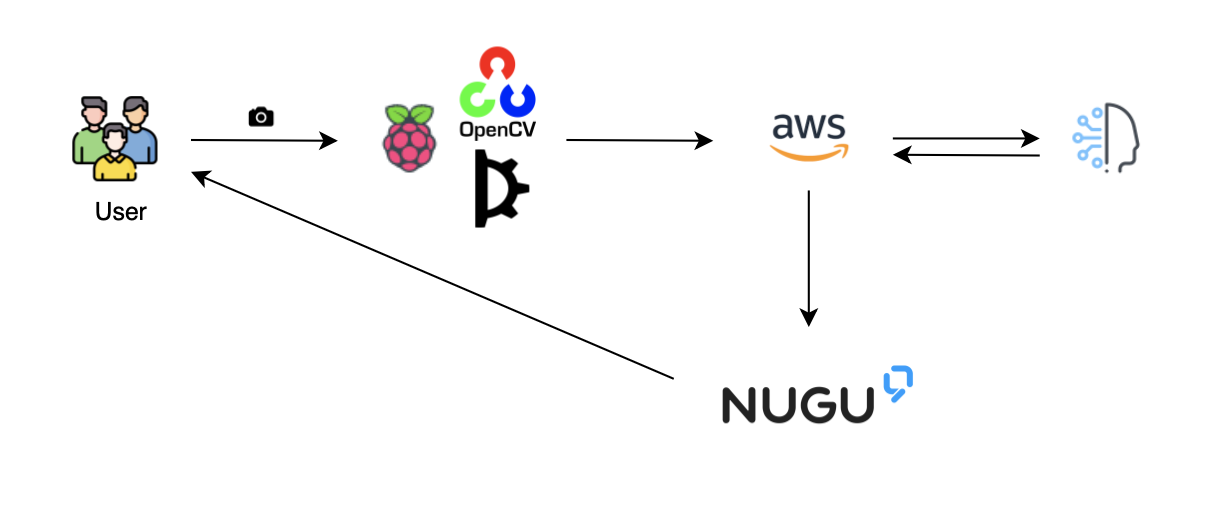
\includegraphics[width=0.5\textwidth]{images/SE-architecture.png}
%\end{figure}

\begin{figure}[h]
    \centering
    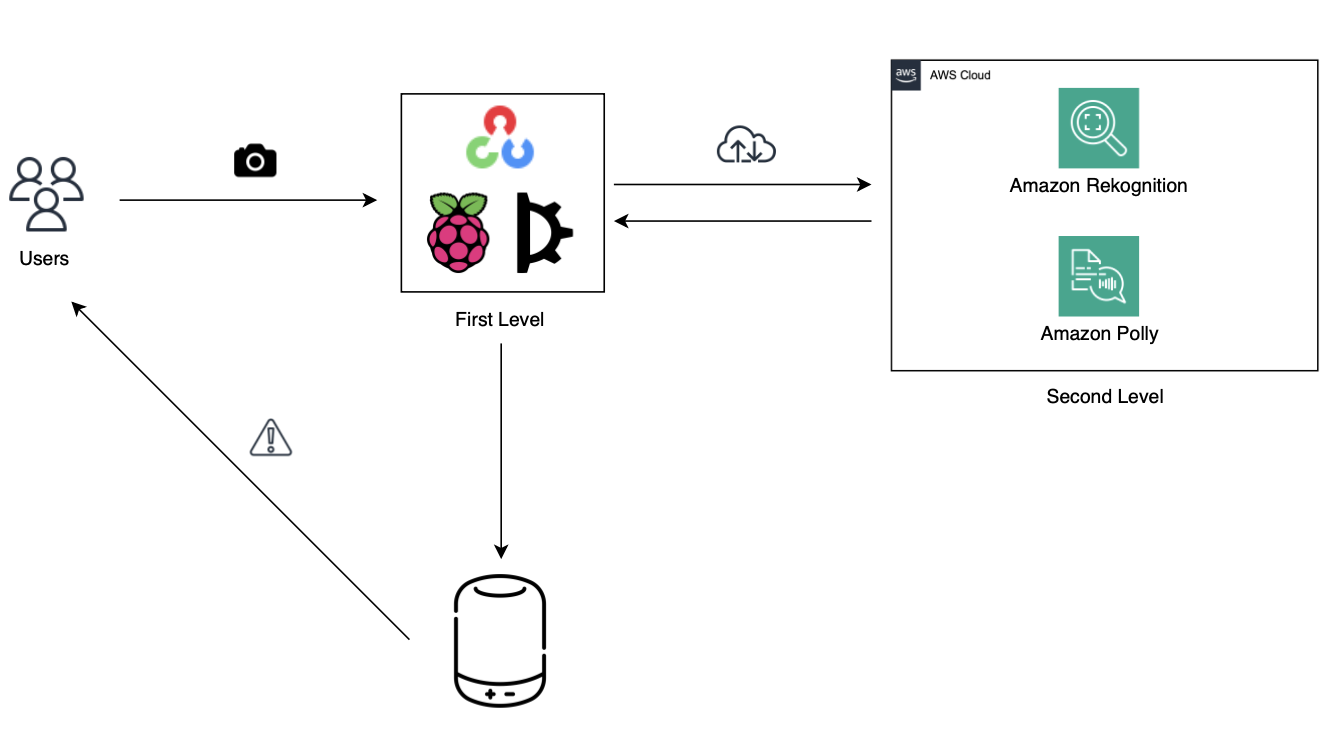
\includegraphics[width=1\linewidth]{images/architecture.png}
    \caption{Project Architecture}
    \label{fig:enter-label}
\end{figure}

\subsection{\textbf{Training AI model}}
% 인공지능 모델을 데이터를 기반으로 학습시키는 과정이다. 데이터는 kaggle의 'Face Images of Acute Stroke and Non Acute Stroke' 의 38MB 가량 이미지이다. Stroke face 이미지 약 1,600장, non stroke face 약 2,400장으로 총 4,000여장의 데이터로 학습을 진행한다. 학습 과정에서 이미지 전처리는 다음과 같이 진행한다. (200x2000x3)의 tensor로 변환하고 flatten 한다. label은 stroke face를 1, non-stroke face를 0으로 표기했고 SVM과 Transformer 모델을 위와 같은 조건에서 Google Colab에서 학습시킨다.
This is the process of learning an artificial intelligence model based on data. The data is a 38MB image from kaggle's 'Face Images of Acute Stroke and Non Acute Stroke'. Training is conducted with a total of 4,000 pieces of data, including about 1,600 stroke face images and 2,400 non-stroke face images. Image preprocessing during the learning process proceeds as follows. Convert to a tensor of (200x200x3) and flatten. The label indicates the stroke face as 1 and the non-stroke face as 0, and the SVM and Transformer models are trained in Google Colab under the above conditions.\\

\subsubsection{\textbf{Support Vector Machine}}
% Support Vector Machine을 사용하기 위해서 scikit-learn에서 svm 라이브러리를 import한다. 설정할 수 있는 hyper parameter는 다음과 같다.
\begin{itemize}
    \item C(Regularization Parameter): C is a parameter that controls the penalty for misclassifications. A small C value sets a low penalty for misclassifications, making the model fit the training data more. A large C value sets a high penalty for misclassifications, encouraging the model to achieve higher accuracy on the training data. The appropriate value for C is determined through cross-validation.
    \item Kernel: SVM supports various kernel functions. The most commonly used kernels include the linear kernel, polynomial kernel, and Radial Basis Function (RBF) kernel. The choice of kernel depends on the data's characteristics and the problem at hand.
    \item Gamma: When using the RBF kernel, Gamma controls the flexibility of the decision boundary. A small Gamma value makes the decision boundary smoother, while a large Gamma value makes the decision boundary more complex. The appropriate value for Gamma is also determined through cross-validation.
\end{itemize}
% 이런 다양한 hyper parameter 중 kernel은 rbf kernel을 사용하고 나머지 두 파라미터를 sklearn 라이브러리의 GridSearchCV method를 사용해 최적의 값을 구한다.

\subsubsection{\textbf{ViT}}
\cite{vision-transformers-medium}
% ViT는 다양한 모듈이 모여 구성된다. 모듈은 다음과 같이 구성된다.
ViT is composed of various modules. The module is composed as follows.\\

\textbf{Patchify} \\
The transformer encoder was developed with sequence data in mind, such as English sentences. However, an image is not a sequence. So we have to “sequencify” an image. We break it into multiple sub-images and map each sub-image to a vector.

We do so by simply reshaping our input, which has size (N, C, H, W), to size (N, \#Patches, Patch dimensionality), where the dimensionality of a patch is adjusted accordingly.\\

\textbf{Adding classification tokens} \\
If you look closely at the architecture picture, you will notice that also a “v\_class” token is passed to the Transformer Encoder.

Simply put, this is a special token that we add to our model that has the role of capturing information about the other tokens. This will happen with the MSA block (later on). When information about all other tokens will be present here, we will be able to classify the image using only this special token. The initial value of the special token (the one fed to the transformer encoder) is a parameter of the model that needs to be learned.

If we wanted to do another downstream task, we would just need to add another special token for the other downstream task (for example, classifying a digit as higher than 5 or lower) and a classifier that takes as input this new token.\\

\textbf{Positional Encoding} \\
As anticipated, positional encoding allows the model to understand where each patch would be placed in the original image. While it is theoretically possible to learn such positional embeddings, previous work by Vaswani et. al. suggests that we can just add sines and cosines waves.

In particular, positional encoding adds high-frequency values to the first dimensions and low-frequency values to the latter dimensions.

In each sequence, for token i we add to its j-th coordinate the following value:


\[p_{i, j} = \left\{\begin{matrix}
sin\left(\frac{i}{10000^{\frac{j}{d_{emb\_dim}}}}\right) \\ cos\left(\frac{i}{10000^{\frac{j}{d_{emb\_dim}}}}\right)
\end{matrix}\right.\]

This positional embedding is a function of the number of elements in the sequence and the dimensionality of each element. Thus, it is always a 2-dimensional tensor or “rectangle”.

Here’s a simple function that, given the number of tokens and the dimensionality of each of them, outputs a matrix where each coordinate (i,j) is the value to be added to token i in dimension j.\\

\textbf{Layer Normalization}
Layer normalization is a popular block that, given an input, subtracts its mean and divides by the standard deviation.

However, we commonly apply layer normalization to an (N, d) input, where d is the dimensionality. Luckily, also the Layer Normalization module generalizes to multiple dimensions.

Layer normalization is applied to the last dimension only. We can thus make each of our 50x8 matrices (representing a single sequence) have mean 0 and std 1.\\

\textbf{Multi-head Self Attention} \\
Simply put: we want, for a single image, each patch to get updated based on some similarity measure with the other patches. We do so by linearly mapping each patch to 3 distinct vectors: \(\mathbf{q}, \mathbf{k}\), and \(\mathbf{v}\) (query, key, value).


Then, for a single patch, we are going to compute the dot product between its q vector with all of the k vectors, divide by the square root of the dimensionality of these vectors, softmax these so-called attention cues, and finally multiply each attention cue with the v vectors associated with the different k vectors and sum all up.

In this way, each patch assumes a new value that is based on its similarity (after the linear mapping to \(\mathbf{q}, \mathbf{k}\) and \(\mathbf{v}\)) with other patches. This whole procedure, however, is carried out H times on H sub-vectors of our current 8-dimensional patches, where H is the number of Heads. If you’re unfamiliar with the attention and multi-head attention mechanisms, I suggest you read this nice post by Yasuto Tamura.

Once all results are obtained, they are concatenated together. Finally, the result is passed through a linear layer (for good measure).

The intuitive idea behind attention is that it allows modeling the relationship between the inputs. What makes a ‘0’ a zero are not the individual pixel values, but how they relate to each other.\\

\textbf{Residual Connection} \\
A residual connection consists in just adding the original input to the result of some computation. This, intuitively, allows a network to become more powerful while also preserving the set of possible functions that the model can approximate.

With this self-attention mechanism, the class token (first token of each of the N sequences) now has information regarding all other tokens.\\

\textbf{Classfication MLP} \\
Finally, we can extract just the classification token (first token) out of our N sequences, and use each token to get N classifications.



\\
\subsection{\textbf{Saving trained AI model}}
% 학습이 완료된 인공지능 모델을 파일로 저장해 웹 서버에 배포할 수 있도록 저장한다. 저장하는 형식은 여러가지가 있다. 우리가 사용한 방식은 joblib이다. joblib은 dump(), load() 명령어로 단순하게 모델을 저장하고 불러올 수 있기 때문에 선택했다. Google Colab에서 학습이 완료된 인공지능 모델을 joblib.dump() 명령으로 Google Drive에 저장하고 local computer로 다운로드한다.
The trained artificial intelligence model is saved as a file so that it can be distributed to a web server. There are various saving formats. The method we used is joblib. joblib was chosen because it allows you to simply save and load models with the dump() and load() commands. Save the artificial intelligence model that has completed training in Google Colab to Google Drive using the joblib.dump() command and download it to your local computer.\\

\subsection{\textbf{Loading trained AI model}}
% 저장한 방식과 같이 joblib 라이브러리를 사용해서 학습이 완료된 인공지능 모델을 파일에서부터 불러올 수 있다. Google Colab에서 인공지능을 학습시키고 저장된 모델을 AWS Lightsail에 scp 명령어를 통해 local에서 옮긴다. 이로써 모델을 AWS Lightsail 가상 머신으로 웹 서버를 이용해 배포할 준비를 마친다.
Just like how you saved it, you can load the trained artificial intelligence model from a file using the joblib library. Train artificial intelligence in Google Colab and move the saved model locally to AWS Lightsail using the scp command. This completes the preparation to deploy the model as an AWS Lightsail virtual machine using a web server.\\

\subsection{\textbf{Classifying Image with trained AI model}}
% 인공지능 모델을 학습시킬 때와 유사하게 이미지를 전처리한다. (200x200x3) tensor로 이미지를 변환한다. skimage 라이브러리의 resize 함수를 호출해 처리한다. 이후 flatten 시켜 이미지 전처리를 완료한다. load 된 인공지능 모델로 predict 메소드를 호출하고 전처리된 이미지를 파라미터로 넘겨줘서 예측값을 반환하도록 한다. 이때, 단순히 0 또는 1의 classification 된 결과뿐만 아니라 각 확률값을 같이 반환하도록 해서 판단의 근거를 사용자에게도 알려준다.
Images are preprocessed similarly to when training an artificial intelligence model. Convert the image to (200x200x3) tensor. Process it by calling the resize function of the 'skimage' library. Afterwards, image preprocessing is completed by flattening. Call the predict method with the loaded artificial intelligence model and return the predicted value by passing the preprocessed image as a parameter. At this time, not only the classified result of 0 or 1 is returned, but also the probability value is returned to inform the user of the basis for the judgment.\\

\subsection{\textbf{Returning the result}}
% 반환된 값을 다시 웹 통신으로 라즈베리 파이로 전송해야 하기 때문에 JSON 객체로 변경한다. 총 3개의 key-value 값으로 이루어져 있다. key는 다음과 같다. 'prediction', 'probability_0', 'probability_1'로 각각 예측값, non-Stroke 확률, Stroke 확률을 나타낸다. 예시 객체는 다음과 같다.
Because the returned value needs to be sent back to the Raspberry Pi via web communication, it is changed to a JSON object. It consists of a total of three key-value values. The key is as follows. 'prediction', 'probability\_0', and 'probability\_1' represent the predicted value, non-stroke probability, and stroke probability, respectively. Example objects are as follows:
\begin{verbatim}
{
    'prediction': result_list[0],
    'probability_0': probability[0][0],
    'probability_1': probability[0][1]
}
\end{verbatim}
\\

\subsection{\textbf{Get Image with API}}
% FastAPI의 File, UploadFile 라이브러리를 이용하면 웹 서버를 통해 전송된 사진을 프로그램 내에서 처리할 수 있다. skimage.io 라이브러리의 imread 메소드와 결합하여 사용하면 training 과정에서와 같은 로직으로 이미지를 인공지능 모델에 전달할 수 있다. 예시 코드는 다음과 같다.
Using FastAPI's File and UploadFile libraries, images sent through a web server can be processed within the program. When used in combination with the 'imread' method of the skimage.io library, images can be transmitted to the artificial intelligence model using the same logic as in the training process. Example code is as follows:
\begin{verbatim}
{
    img_array = imread(file.file)
}
\end{verbatim}
\\
\subsection{\textbf{Post the result with API}}
% 위의 Returning the result에서 Json format으로 예측값을 변환하여 만든 값을 다시 라즈베리 파이로 보내준다. @app.post("/classify/") annotation이 붙어있는 함수에서 return을 하게 되면 해당 이미지 파일을 보내준 곳으로 응답을 보내기 때문에 classification을 하는 함수 위에 해당 annotation을 붙이고 위의 Json format을 return 하면 Post할 수 있다.
In 'Returning the result' above, the predicted value is converted to JSON format and the resulting value is sent back to the Raspberry Pi. When you return from a function with the @app.post("/classify/") annotation, a response is sent to the place where the image file was sent, so if you attach the annotation to the function that performs classification and return the above Json format, you can Post.\\

\subsection{\textbf{Encapsulate the AI model}}
% 위에서 언급한 모든 내용을 한 파일로 구현할 수 있다. app.py 파일을 제작하고 이미지 전처리, 인공지능 모델에서의 prediction, return값을 제작하고 이 함수 위에 annotation을 붙여 모든 일을 한번에 처리하도록 encapsulation 할 수 있다.
Everything mentioned above can be implemented in one file. You can create an app.py file, create image preprocessing, prediction from an artificial intelligence model, and return value, and attach an annotation on top of this function to encapsulate it so that all tasks are processed at once.\\

\subsection{\textbf{Run the Web Server}}
% Uvicorn 으로 app.py 파일을 실행할 수 있다. 이 때, 외부 IP도 접속 가능하도록 아래와 같이 추가 명령어를 기입해 실행한다.
You can run the app.py file with Uvicorn. At this time, enter and execute the additional command as shown below to enable connection to the external IP.
\begin{verbatim}
    uvicorn app:app --reload --host=0.0.0.0
\end{verbatim}


\subsection{\textbf{Amazon Rekognition}}
\subsubsection{\textbf{Preparing Data}}
% 학습에 필요한 데이터는 이전과 동일하게 stoke data 1200개 가량, no_stroke data 2500개 가량으로 총 3700 여개로 구성되었다. Amazon Rekogniton에서는 데이터가 속한 폴더의 이름을 이미지의 레이블로 자동으로 설정할 수 있다. 이 기능을 이용해 편리하게 데이터의 라벨링을 완료했고 학습용 데이터와 테스트용 데이터를 8:2의 비율로 나누었다. 따로 이미지의 색을 흑백으로 바꾸거나 이미지의 사이즈를 통일시키는 작업은 처리하지 않았다.
The data needed for learning was the same as before, consisting of approximately 1,200 stroke data and 2,500 no\_stroke data, for a total of 3,700 pieces. Amazon Rekogniton can automatically set the name of the folder containing the data as the label of the image. Using this function, we conveniently completed labeling the data and divided the training data and testing data in a ratio of 8:2. No work was done to change the color of the image to black and white or to unify the size of the image.

\begin{figure}[h]
    \centering
    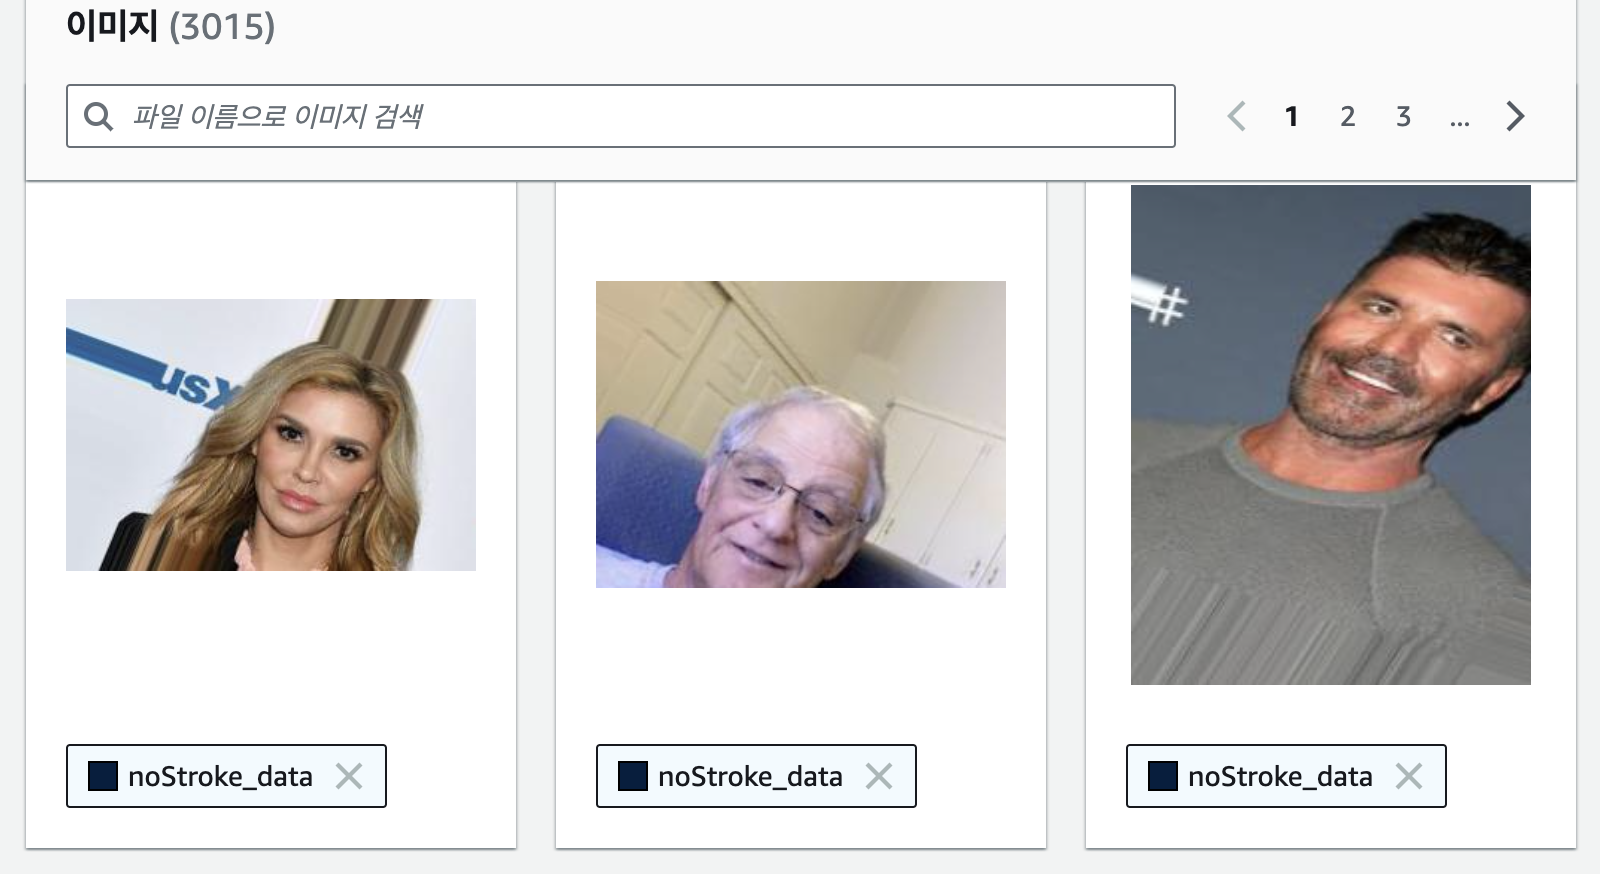
\includegraphics[width=8.5cm]{images/rek_data.png}
    \caption{Dataset for training Amazon Rekognition}
\end{figure}


\subsubsection{\textbf{Training Rekognition model}}
% 위에서 준비한 데이터로 Amazon Rekognition 모델을 학습시킨다. 하이퍼파라미터나 추가적으로 설정해야하는 것들은 자동으로 설정하고 그 중에서 최적의 파라미터를 자동으로 찾아주기 때문에 optimizer나 파라미터를 설정하지 않고 바로 모델 훈련을 진행했다.
Train the Amazon Rekognition model with the data prepared above. Hyperparameters and those that need to be set additionally are automatically set and the optimal parameters are automatically found, so model training was performed immediately without setting the optimizer or parameters.


\begin{figure}[h]
    \centering
    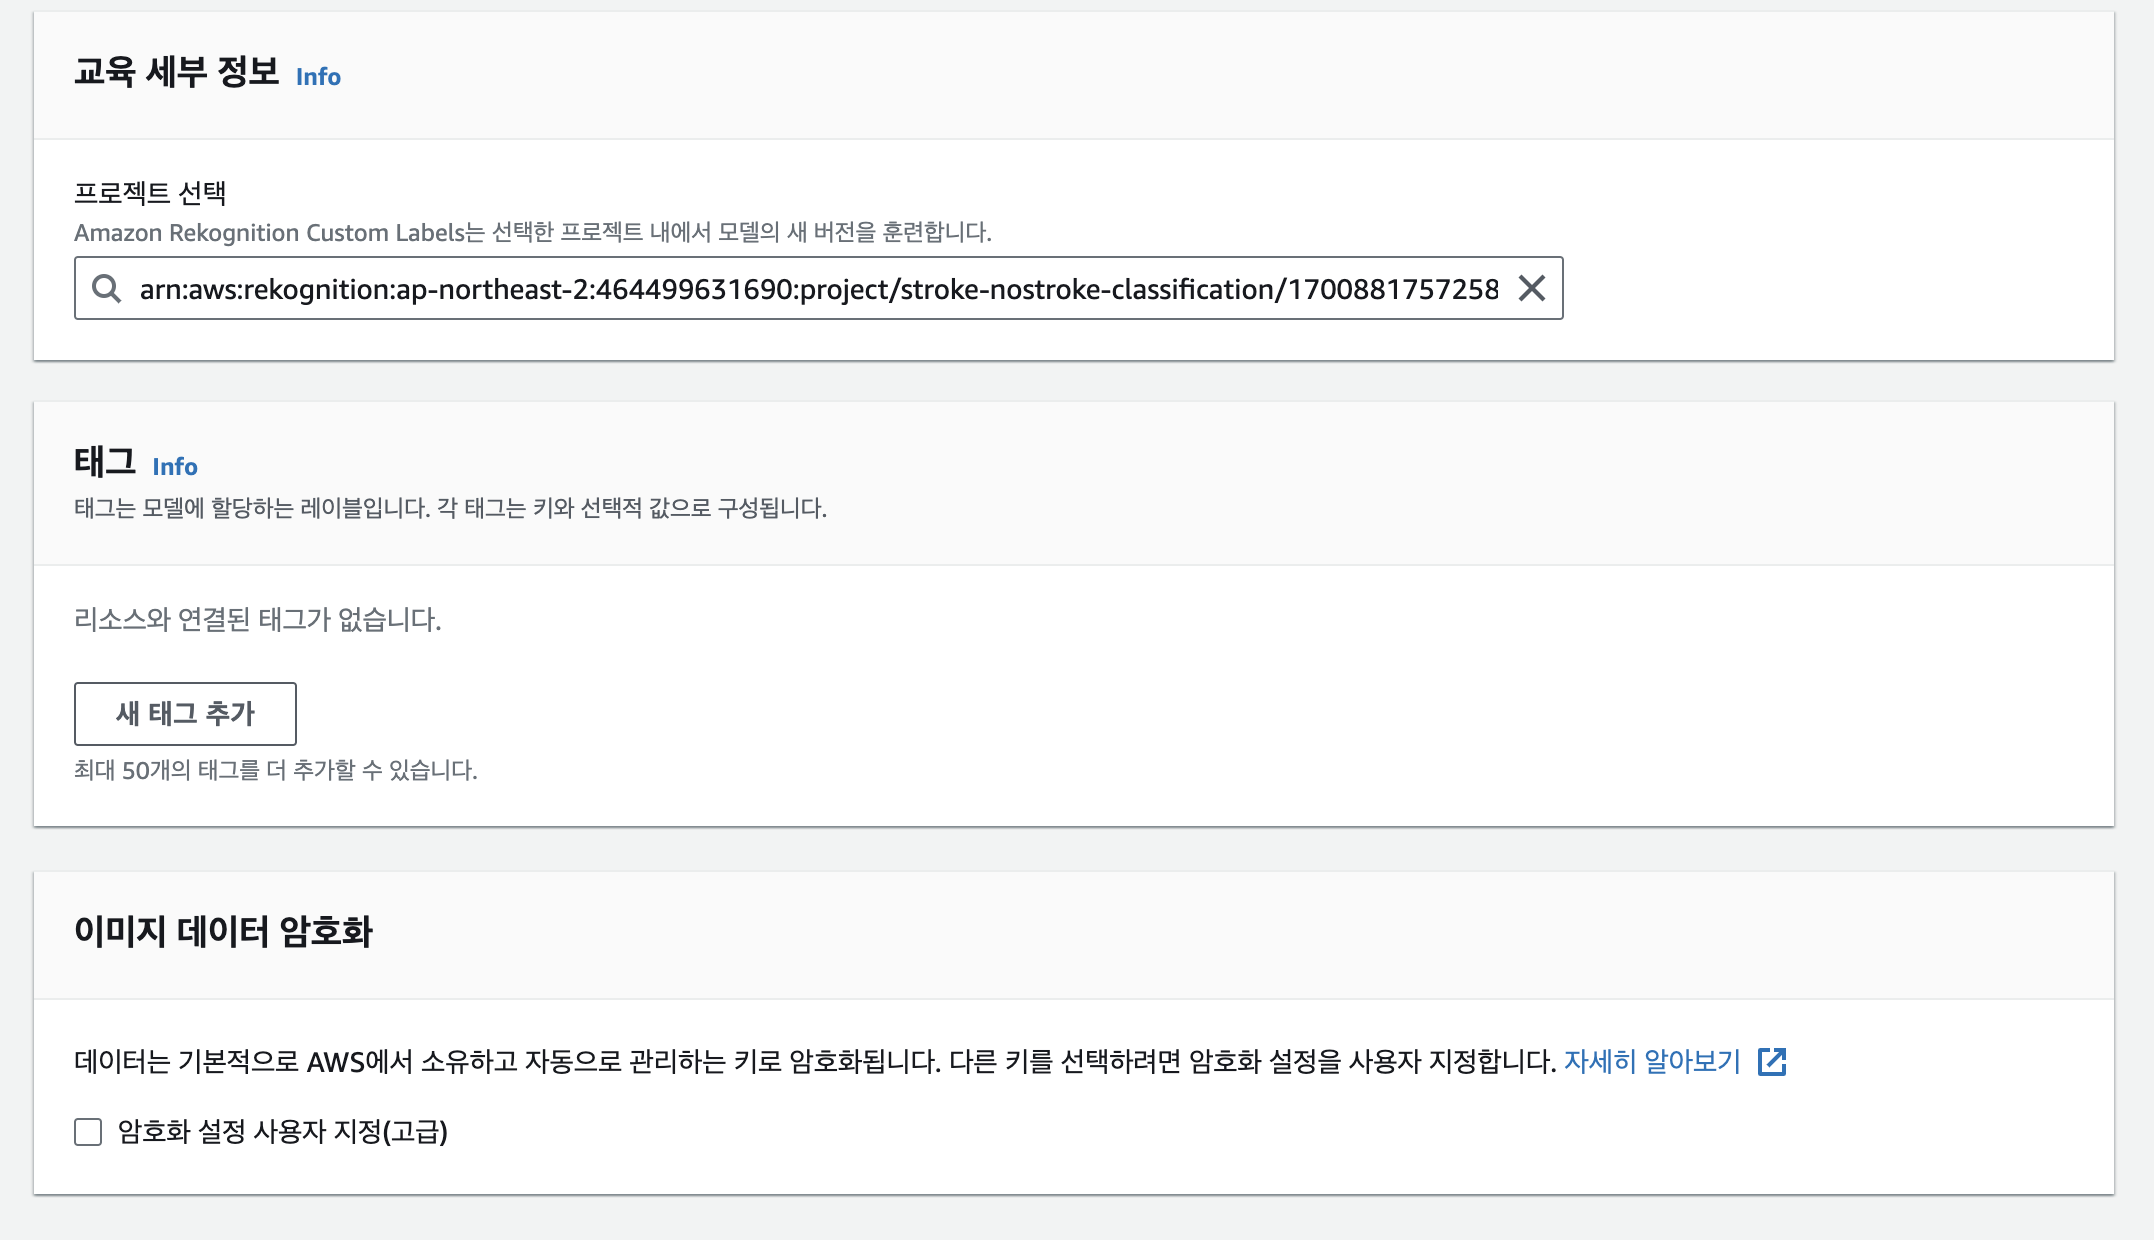
\includegraphics[width=8.5cm]{images/rek_training.png}
    \caption{Training Amazon Rekognition, Full automatic}
\end{figure}


\subsubsection{\textbf{Testing and Deploying trained model}}
% 모델의 학습이 종료되면 배포할 수 있다. 이로써 외부에서 학습된 모델에 접근할 수 있고, 따로 웹 서버를 만들고 실행할 필요 없다. 배포 전에 학습된 모델의 성능을 테스트한 결과도 볼 수 있다. 테스트 데이터 상에서 모든 결과를 정확하게 분류했다. 아래에서 볼 수 있듯이 F1 score 가 1이 나왔다. 그리고 각 데이터의 Confidence level도 상당히 높은 것으로 보아 모델의 학습이 매우 잘 이루어졌단 것을 알 수 있었다.

Once training of the model is complete, it can be distributed. This allows access to externally trained models, and there is no need to create and run a separate web server. You can also see the results of testing the performance of the learned model before deployment. All results were accurately classified on the test data. As you can see below, the F1 score was 1. Also, the confidence level of each data was quite high, showing that the model was trained very well.
\begin{figure}[h!]
    \centering
    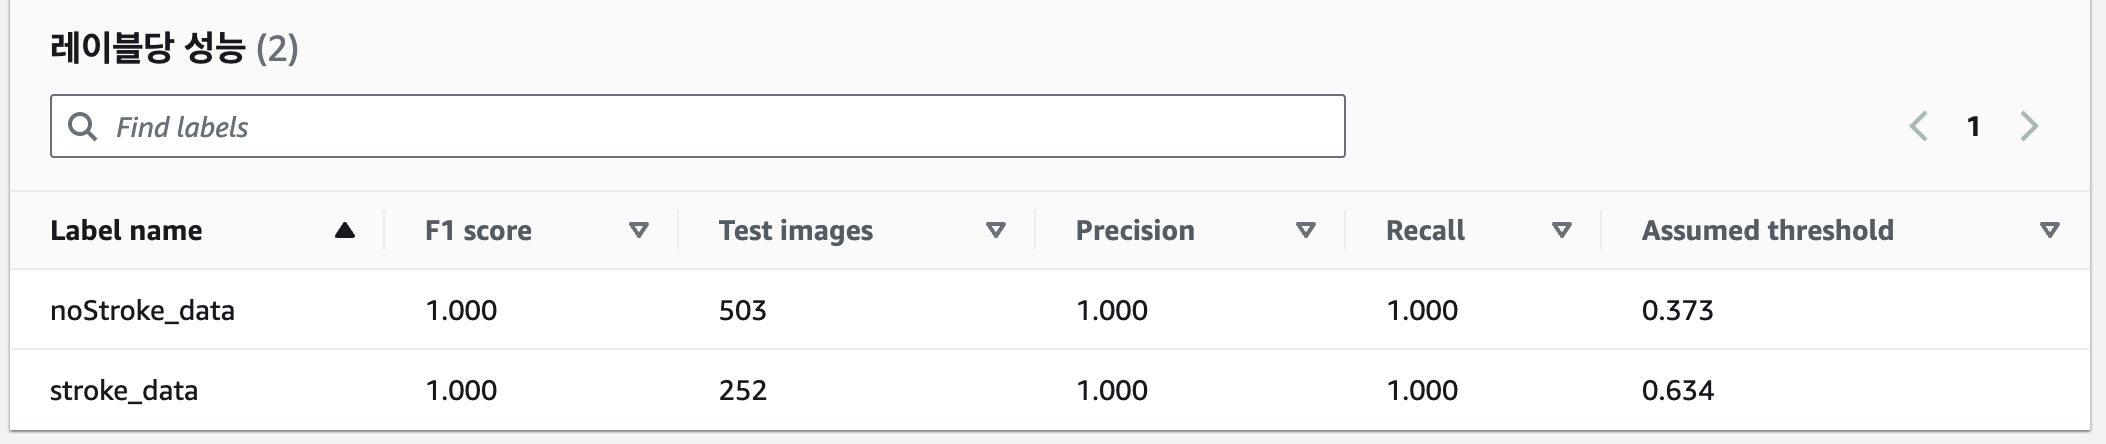
\includegraphics[width=8.5cm]{images/rek_result.png}
    \caption{Result of testing trained Rekogniton model}
\end{figure}


\begin{figure}[h!]
    \centering
    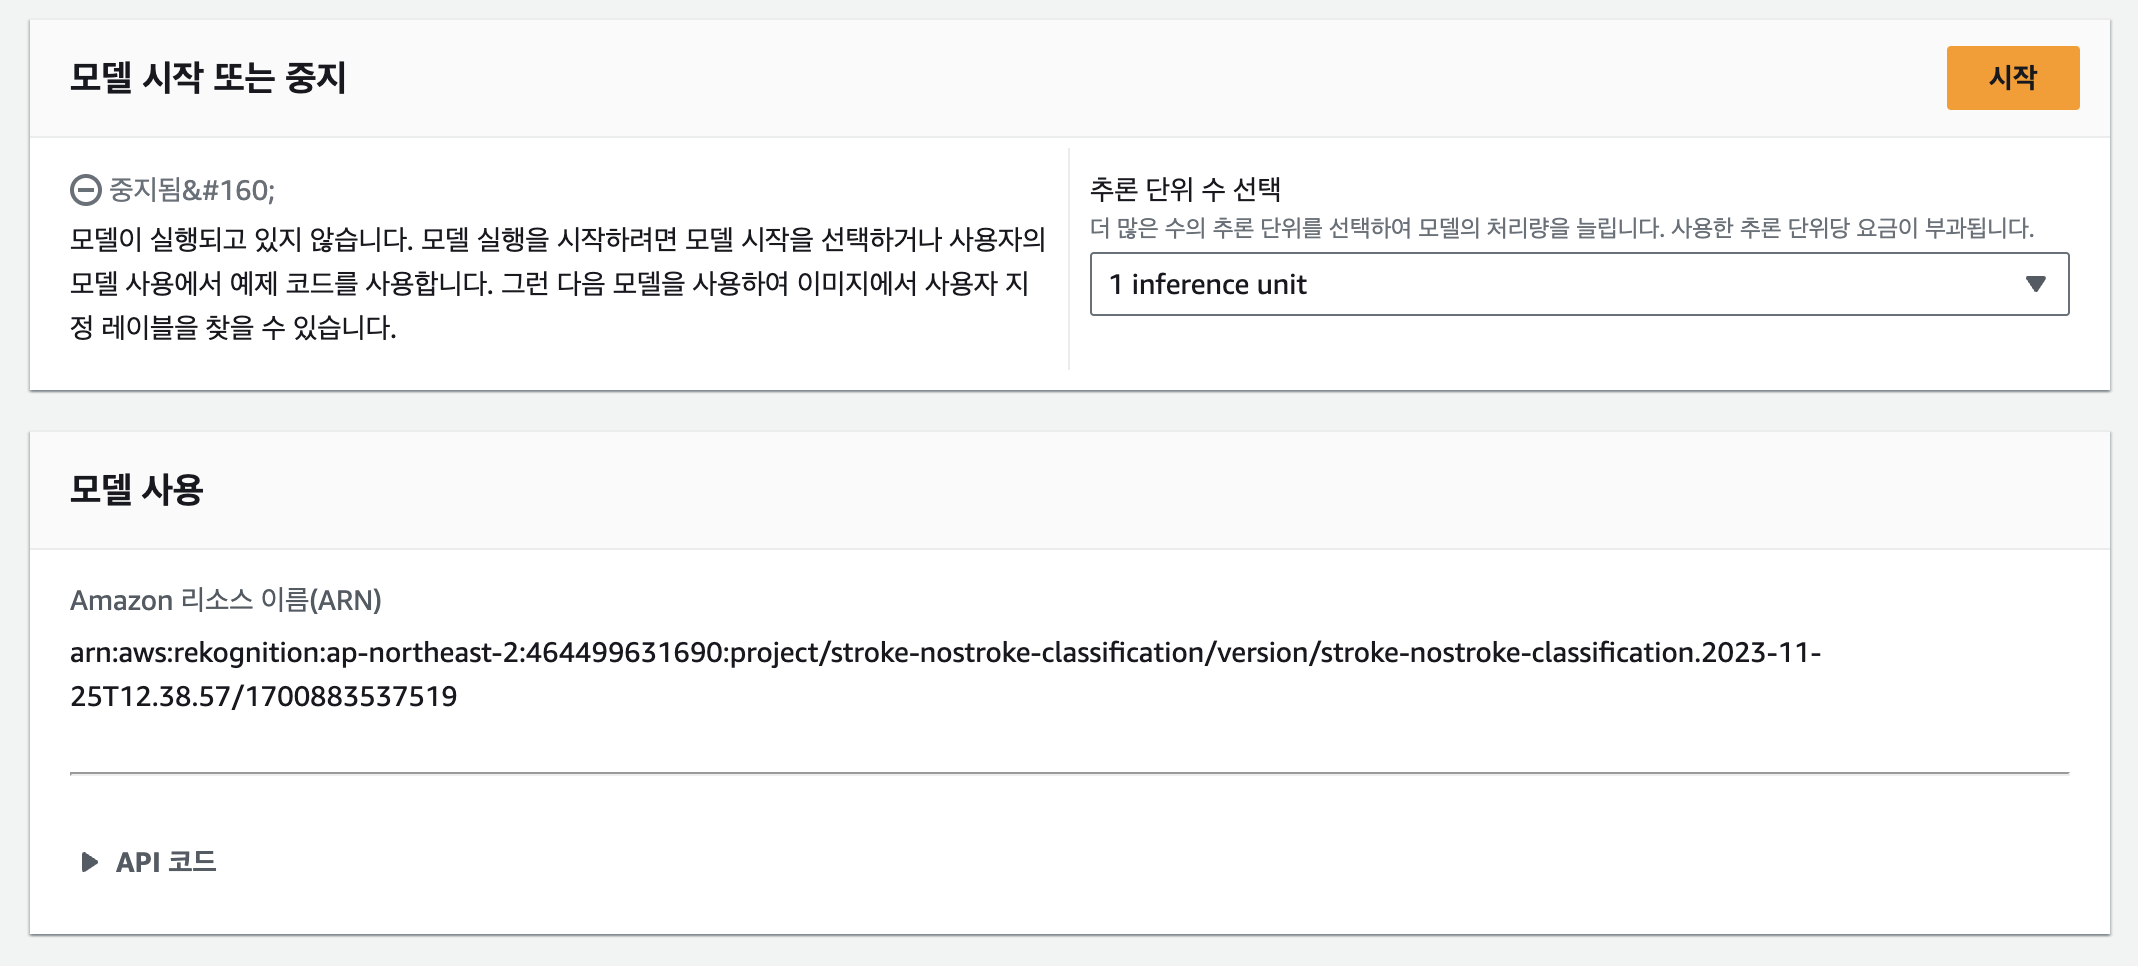
\includegraphics[width=8.5cm]{images/rek_deploy.png}
    \caption{Deploying trained Rekognition model}
\end{figure}



\subsection{\textbf{Raspberry Pi}}

\subsubsection{\textbf{Raspberry OS installation and connection}}
To download the Raspberry Pi OS image, you will need a micro SD card. Recently, with the introduction of the Raspberry Pi Imager, downloading and installing the OS has become more convenient.
First, download the Raspberry Pi Imager on your local desktop. Then, insert the micro SD card into your desktop. In the Raspberry Pi Imager, select the SD card from the Storage tab and install the Raspberry Pi OS.
After that, insert the SD card into the Raspberry Pi, and connect the power using a USB-C port. Your Raspberry Pi will power on.\\

\subsubsection{\textbf{Wi-fi}}
\begin{figure}[h]
    \centering
    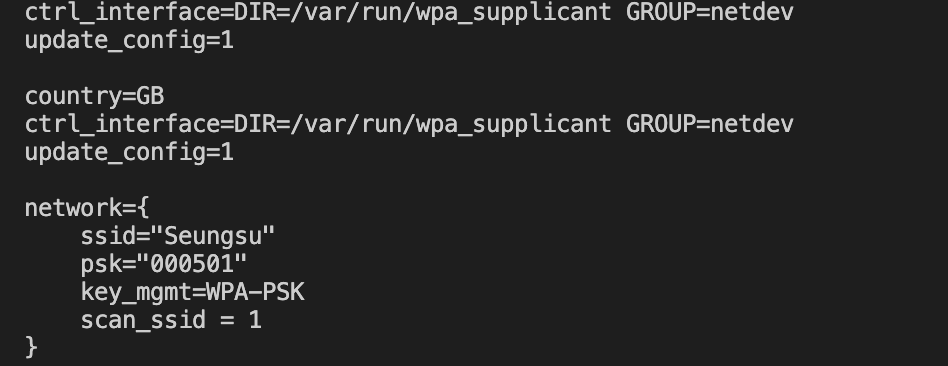
\includegraphics[width=1\linewidth]{images/wifi.png}
    \caption{Wifi Setting}
    \label{fig:enter-label}
\end{figure}
While Raspberry Pi does have a built-in Wi-Fi module, it doesn't automatically connect during boot. To enable this functionality, you need to modify the 'wpa\_supplicant.conf' file. Insert your Wi-Fi ID and password as shown below, and use 'scan\_ssid = 1' to allow detection of hidden networks. By making these changes to the 'wpa\_supplicant.conf' file, Raspberry Pi will automatically connect to Wi-Fi during boot. Wi-Fi connection is crucial not only for internet access but also for SSH usage.\\

\subsubsection{\textbf{SSH}}
You can configure SSH in the Raspberry Pi settings. Enabling SSH automatically completes the necessary settings. After that, when you first establish an SSH connection, set the connection password, and you are ready to use SSH.
\\

SSH primarily relies on IP for forwarding, so you need to know the current IP address of the Raspberry Pi, which you can check by entering 'ifconfig' in the terminal. Additionally, the local and remote devices you want to connect must be connected to the same Wi-Fi network by default.
After connecting your local desktop to the same Wi-Fi network as the Raspberry Pi, you can complete the SSH connection by entering 'ssh userID@xxx.xx.xx.x,' providing your username and IP address, and entering the password.\\

\subsubsection{\textbf{Camera}}
\begin{figure}[h]
    \centering
    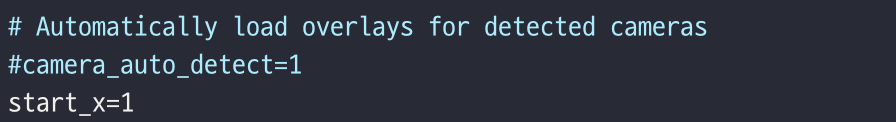
\includegraphics[width=1\linewidth]{images/camera.png}
    \caption{Camera Setting}
    \label{fig:enter-label}
\end{figure}
With the update of the Raspberry Pi OS to 'Bookworm,' there have been changes in the overall software for using the camera. The update involved transitioning to the 'libcamera' library, which posed challenges when applying it to essential camera functions, such as 'VideoCapture' in OpenCV. Therefore, it is necessary to revert to the previous version.

In the 'config.txt' file, you should provide the 'start\_x=1' parameter and turn off the 'camera\_auto\_detect' feature.\\

\subsubsection{\textbf{Virtual Environment for Python}}
Raspberry Pi is an externally managed environment, and as such, it restricts the use of 'pip,' allowing only 'apt' for package management. However, creating a Python virtual environment can provide more flexibility within these constraints. A significant reason for using Python is the availability of a wide range of libraries. To conveniently install these libraries, it is advisable to create a virtual environment.\\

\subsubsection{\textbf{Swap size}}
OpenCV is a sizable library, and to ensure stable operation, it's important to allocate sufficient disk space. You can determine the current swap size in use by using 'free -m.' Then, you can adjust the swap size by modifying '/etc/dphys-swapfile.' The default setting is 100, but to ensure normal operation, it's recommended to set it to 4096 or higher. After adjusting the swap size, you can proceed with the installation of OpenCV\\

\subsection{\textbf{OpenCV}}
\subsubsection{\textbf{video\_capture}}
 to use the 'VideoCapture' function properly, you need to downgrade the camera library and disable 'camera\_auto\_detect' to use OpenCV/V4L2. Additionally, increasing the GPU memory on the Raspberry Pi is recommended for improved video processing.\\

 \subsubsection{\textbf{Color scale converting}}
Using 'cv2.cvtColor,' the image being captured is converted to grayscale. This is used for the following reasons:\\

\begin{itemize}
\item Information Compression: Grayscale images have only one color channel per pixel, representing only brightness information. This reduces image size, saving memory and reducing computational requirements for storage and processing.\\
\item Computational Efficiency: Grayscale image processing is much faster and more efficient compared to color image processing. Handling a single color channel is faster and more efficient than multiple color channels.\\
\item Feature Extraction and Object Detection: Grayscale images are primarily used in image processing tasks such as edge detection, feature extraction, and object detection. Edge detection algorithms often rely on brightness information, making grayscale images more suitable for these tasks.\\
\item Memory Savings: Grayscale images require less memory compared to color images, which can be advantageous for memory-intensive tasks, such as deep learning models.\\
\end{itemize}

Facial recognition is possible with grayscale images, so changing to grayscale helps increase computational efficiency.\\

\subsection{\textbf{Amazone Polly}}
\subsubsection{AWS Account and IAM User Setup:}
Log in to the AWS Management Console.
Create an IAM user with the necessary permissions to use the Polly service. Assign the user the appropriate policies to allow Polly API calls.
\subsubsection{Install Boto3 Library:}
Install the boto3 library for Python, which is required for interacting with AWS services.
\subsubsection{Play the speach file:}
Depending on our device, Raspberry pi, We can use tools like pygame or cvlc to play the generated MP3 file.



\subsection{\textbf{Privacy Policy}}
To ensure personal data protection, we implement a two-step process:\\

\begin{enumerate}
    \item The first step involves blurring the background screen.
    \begin{enumerate}
    \item Backgroung Blur\\
    \end{enumerate}
    
    \item The second step uses a computer vision model that operates exclusively on the local device for initial assessment. Only if detection is made, the connection to the server is established. we called it 'Two-level detection'.
And if connected to the internet, an LED module lights up next to the camera, allowing customers to visually confirm whether the camera is online or not.\\
\\
    \textbf{Two-level detection:}
    \cite{gradient} Through the following research paper, we obtained the gradient difference at the corner of the mouth for stroke diagnosis using face detection. Utilizing the coordinates of each landmark obtained above, we issue a warning when the gradient exceeds a certain threshold.\\
    
    \begin{enumerate}
    \item \textbf{When No Detection Occurs in Fisrt-level:}\\
\\In the absence of detection in real-time, the system continues to operate actively within the user's daily life without any specific signals.\\
\item \textbf{When Detection Occurs in First-level:}\\
\\Upon detecting risk factors in real-time, the system establishes a connection to the server and captures a more accurate photo for further detection using a trained artificial intelligence model (e.g., SVM, Transformer), ensuring higher accuracy.\\
\item \textbf{When the Diagnosis indicates a Stroke in Second-level:}\\
\\In the event of a stroke diagnosis, the user is promptly informed.
After the notification, the system seeks the user's consent, and upon receiving it, automatically initiates a 119 emergency call.\\
\item \textbf{When the Diagnosis Indicates No Stroke:}\\
\\If no detection occurs in the initial assessment, the system continues its operation. However, in the secondary assessment, if no detection takes place, the user is informed to provide reassurance.

    \end{enumerate}
\end{enumerate}
\usepackage{graphicx}

\section{\textbf{Architecture Design \& Implementation}}

% 다음은 우리의 전체적인 디자인을 다이어그램으로 도식화한 것이다.


\subsection{\textbf{Overall architecture}} \\
% 우리의 디자인은 크게 두 단계로 나뉜다. 카메라로 사람의 얼굴이 감지되었을 때 실시간으로 face drooping을 검사하는 1단계, 1단계에서 의심스러운 정황이 나타나면 좀 더 정밀한 판단을 위해 인공지능 모델에 정확한 사진을 보내서 답을 얻는 2단계로 구성되어 있다. 이렇게 2-level로 검진 시스템을 구축한 이유는 다음과 같다. 첫째, 컴퓨팅 리소스를 낭비하지 않는다. 실시간으로 카메라의 장면을 인공지능 서버에 보내서 검증하기에는 많은 자원이 낭비된다. 또한, 사람이 집 안에서 생활하면 다양한 각도로 찍힐텐데 이런 상황에서 face-drooping으로 잘못 인식할 수 있다. 이런 오류에 컴퓨팅 리소스를 낭비하지 않기 위해 우선 1단계에선 정밀성은 떨어지더라도 라즈베리 파이에서 구동 가능한 정도의 검증 시스템을 구축해 얼굴의 비대칭 정도가 임계값을 넘을 때에만 2단계의 정밀 검증 시스템으로 넘어가도록 했다. 둘째, 개인정보를 보호할 수 있다. 집의 가구에 설치되는 카메라는 필연적으로 개인정보에 민감할 수 밖에 없다. 그래서 사진을 언제 촬영하는지 사용자에게 시각적으로 알려주는 방식을 생각했다. 애플의 맥북 같은 경우, 웹캠이 작동되면 언제나 초록색 불빛이 들어온다. 마찬가지로 우리의 시스템 역시 사진이 촬영될 때는 하드웨어적으로 불빛이 들어오도록 구현해 사생활 침해의 요소를 줄일 수 있다. 셋째, IoT 기기 의 성능을 고려했다. 가구에 탑재되는 IoT 기기는 성능이 충분하지 않다. 이런 기기에 너무 많은 기능을 한번에 탑재하면 전기가 많이 필요하고 이는 가구의 전기 효율은 낮추는 결과를 낳는다. 이를 방지하면서 추후 MLOps를 구축하는데는 인공지능 모델은 2단계로 구분하는 것이 더 낫다고 판단했다.

\begin{figure}[h]
    \centering
    \includegraphics[width=8.5cm]{images/무제.drawio.png}
    \caption{Overall Design of 2-Level}
\end{figure}

Our design is divided into two main steps. It consists of a first stage where the camera checks for face drooping in real-time a person's face is detected, and a second stage where the photo is sent to an artificial intelligence model for more precise details to get an answer since suspicious circumstances are omitted in the first stage. The reason for establishing this two-stage inspection system is as follows.

First, it doesn't waste computing resources. It wastes a lot of resources to send camera scenes to an artificial intelligence server for verification in real time. Additionally, if a person lives inside the house, they will be photographed from various angles, and in this situation, it can be mistaken for face-drooping. In order to avoid wasting computing resources on such errors, we first built a verification system that can be run on a Raspberry Pi even if the accuracy is low in the first stage, and moves to the second stage of precision verification system only when the degree of facial asymmetry exceeds the threshold.

Second, personal information can be protected. Cameras installed on home furniture are inevitably sensitive to personal information. So, I thought of a way to visually inform the user when a photo was taken. In the case of Apple's MacBook, a green light always comes on when the webcam is activated. Likewise, our system is also implemented in hardware to turn on lights when a photo is taken, thereby reducing the element of privacy infringement.

Third, the performance of IoT devices was considered. IoT devices mounted on furniture do not have sufficient performance. If these devices are equipped with too many functions at once, they require a lot of electricity, which results in lowering the electrical efficiency of the household. To prevent this and build MLOps in the future, we decided that it would be better to divide the artificial intelligence model into two stages.\\  

%%%%%%%%%%%%%%%%%%%%%%%%%%%%%%%%%%%%%%%%%%%%%%%
% 라즈베리파이 쓴 이유 조금 더 구체적으로 추가하기
% 1단계의 작동 방식을 간단하게 알아보자. 1단계에서는 비디오 스트림을 이용해 실시간으로 face drooping을 감지한다. face landmark를 이용하여 drooping을 판단하는 값이 임계값을 초과하게 되었을 시 알림을 보내며 2단계로 보낼 사진을 찍는다. 이후 저장된 사진을 2단계에 전송하게 된다.

Let's take a quick look at how Step 1 operates. In this step, real-time face drooping is detected using a video stream. If the calculated value for drooping, based on face landmarks, exceeds a set threshold, an alert is sent, and a photo for Step 2 is taken. This captured photo is then sent to Step 2.\\
The threshold is determined through \cite{mvalue}the examination of the positional relationship between the coordinates of the outer edges of both left and right lips and the midpoint beneath the lower lip. This methodology draws inspiration from the findings of precedent studies and has been configured accordingly. In Step 1 detection, this value is obtained using face landmarks. However, using the m-value of 0.16 as suggested by research resulted in overly sensitive reactions due to the characteristics of the video stream. Therefore, the value was adjusted to 0.2, and its reliable operation was empirically confirmed through multiple simulations.

\begin{equation} 
	m = \frac{y_2-y_1}{x_2-x_1}
\end{equation}

\begin{equation}
    threshold = |m_l - m_r|
\end{equation}

% 이 임계값은 왼쪽과 오른쪽 각 입술 끝 좌표와 아랫입술에서의 가운데 좌표와의 관계를 통해 구해지며 선행 논문의 결과를 참조해 설정하였다.(논문 레퍼런스 및 m value구하는 식 넣기). 1단계 detection에서는 이 값을 face landmark를 이용해 구한다. 다만, 연구 결과대로 m-value를 0.16으로 사용할 시 Video stream의 특성상 너무 예민하게 반응하는 문제가 있었다. 따라서 값을 0.2 수정하였고 신뢰도 있게 작동함을 여러 시뮬레이션을 통해 경험적으로 알 수 있었다.


% 2단계의 작동 방식을 간단하게 알아보자. 2단계에서는 라즈베리파이에서 전달 받은 이미지를 뇌졸중인지 아닌지로 정확하게 판단해야 한다. 이미지 분류 알고리즘을 훈련시키고 이를 검증하고 배포한다. 이 과정에서 훈련과 검증 단계는 더욱 low level적인 이야기이므로 생략한다. 배포 과정은 AWS의 AI 서비스 중 하나인 Amazon Rekognition이나 uvicorn을 사용한다. 이 중 Amazon Rekognition은 모델의 훈련, 검증, 배포를 한번에 진행할 수 있게 도와준다. uvicorn을 이용해서 웹 서버를 열어서 배포를 하는 경우, 입력은 이미지 파일을 받고 flatten시켜 모델의 입력값으로 넘겨준다. 반환값은 0 또는 1과 각각의 판단 확률값이다. 이때 반환값은 각각 no stroke, stroke이다. Amazon Rekognition을 이용했을 때의 입력은 똑같이 이미지 파일이다. 하지만 다른 점은 명시적으로 flatten시키지 않고 반환값은 string으로 'stroke_data' 혹은 'noStroke_data'와 각 판단의 Confidence 값이다.

Let’s take a quick look at how step 2 works. In the second step, the image received from the Raspberry Pi must be accurately judged as to whether it is a stroke or not. Train an image classification algorithm, verify it, and deploy it. In this process, the training and verification stages are omitted as they are more low-level. The deployment process uses Amazon Rekognition or uvicorn, one of AWS's AI services. Among these, Amazon Rekognition helps you train, verify, and deploy the model all at once.
When opening and distributing a web server using uvicorn, an image file is received as input, flattened, and passed as an input value to the model. The return value is 0 or 1 and the respective judgment probability value. At this time, the return values are no stroke and stroke, respectively. The input when using Amazon Rekognition is the same image file. However, the difference is that it is not explicitly flattened, and the return value is a string of 'stroke\_data' or 'noStroke\_data' and the confidence value of each judgment.\\

\begin{figure}[h]
    \centering
    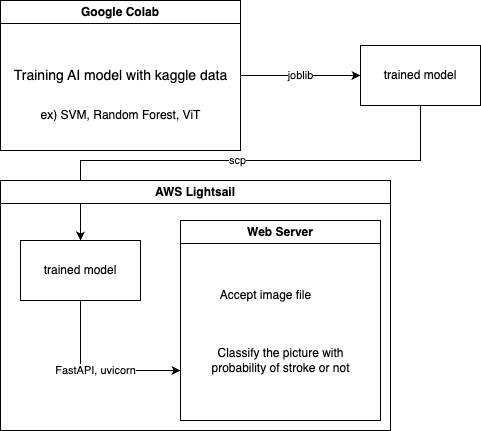
\includegraphics[width=8.5cm]{images/ai-back.drawio (1).png}
    \caption{Architecture when using no-AWS AI service}
\end{figure}


% MLOps를 위한 구현을 살펴보자. AWS를 사용한 이유는 추후의 확장성을 위해서이다. AWS Sagemaker를 이용하면 머신러닝 모델의 학습을 완전 자동화하거나 이미 존재하는 파편화된 코드들을 모아서 파이프라이닝 할 수 있다. 이런 작업을 거치면 ... 우리는 일회성으로 뇌졸중만 판단하는 시스템을 만들고 끝이 아니라 이를 바탕으로 더 거대한 하나의 생태계를 만들 수 있다. 그 기반에는 MLOps가 필수적이다. 데이터 과학자, 데이터 엔지니어, 직무 전문가, 머신러닝 아키텍트 전부 하나의 작업 환경 아래에서 작업할 수 있고, 자동화한다. 이를 바탕으로 다른 새로운 질병을 예측하는 머신러닝 기반 기기를 쉽게 제작하고, 훈련, 배포를 할 수 있다. 이런 생태계를 구축해 놓음으로써 의료, 건강 부분에서 머신러닝 기반 고객 관리 시스템을 쉽게 만들 수 있다.
Let's look at the implementation for MLOps. The reason for using AWS is for future scalability. Using AWS Sagemaker, you can completely automate the learning of machine learning models or pipeline existing fragmented codes. By going through this work... we can create a system that only judges strokes on a one-time basis and create a larger ecosystem based on this. MLOps is essential for that foundation. Data scientists, data engineers, job experts, and machine learning architects can all work under one work environment and automate it. Based on this, machine learning-based devices that predict other new diseases can be easily created, trained, and distributed. By establishing this ecosystem, it is possible to easily create a machine learning-based customer management system in the medical and health sectors.


\subsection{Directory structure}

\begin{table}[h]
\caption{Directory Structure}
\begin{tabular}{|p{4cm}|p{3cm}|p{2cm}|}
\hline
Directory & File names & Module names in use \\ \hline
/Raspberry/First\_level\_detection & first\_level.py & First\_level detection \\ \hline
/Raspberry/First\_level\_detection & detect\_face.py & First\_level detection\\ \hline
/Raspberry/First\_level\_detection & take\_photo.py & First\_level detection\\ \hline
/Raspberry/First\_level\_detection & image\_send.py & First\_level detection\\ \hline
/Raspberry/First\_level\_detection & count\_clock.py & First\_level detection\\ \hline
/Raspberry/First\_level\_detection & send\_aws.py & First\_level detection\\ \hline
/Raspberry/First\_level\_detection & voice\_alert.py & First\_level detection\\ \hline
model/AWS-Rekognition   &    classifier.py        &      AI-back  \\ \hline
model/Random-Forest   &  SE\_RandomForest.ipynb rf\_stroke\_classification       &   AI-back   \\ \hline
model/SVM   &     SE\_SVM.ipynb se\_svm.py      &          AI-back        \\ \hline
model/ViT   &      SE\_ViTprac.ipynb \newline se\_vitprac.py     &          AI-back \\ \hline
model/deployment & app.py & AI-back \\ \hline
\end{tabular}
\end{table}

\subsubsection{Module1: First\_level detection}
%1단계 detection은 face landmark를 이용한다. 이것은 Video stream을 이용해 실시간으로 정보를 처리하며, 뇌졸중의 징후인 mouth droop이 보일 때 사진을 찍어 2단계 모델로 전송한다. 1단계 detection은 징후가 조금이라도 포착되면 작동하기 때문에 정확도가 높지 않다. 신뢰도 있는 판정은 2단계에서 해주므로 1단계 detection의 의의는 real-time 처리 및 자원 사용의 효율성 및 개인 정보 보호로 볼 수 있을 것이다. 다만, IoT에 적용될 프로그램을 생각하면서 만들었기에 한정된 자원의 효율적 사용 또한 매우 중요한 지점이 될 것이다.
Step 1 detection relies on face landmarks, processing real-time information through a video stream. It takes a photo when it detects signs of mouth drooping, indicative of a stroke, and sends it to the Step 2 model. Since Step 1 activates upon detecting even slight indications, its accuracy may not be very high. The significance of Step 1 detection lies in its real-time processing, efficient use of resources, and privacy protection. However, given its design for application in IoT programs, the efficient use of limited resources is also a critical consideration.\\


\begin{figure}[h]
    \centering
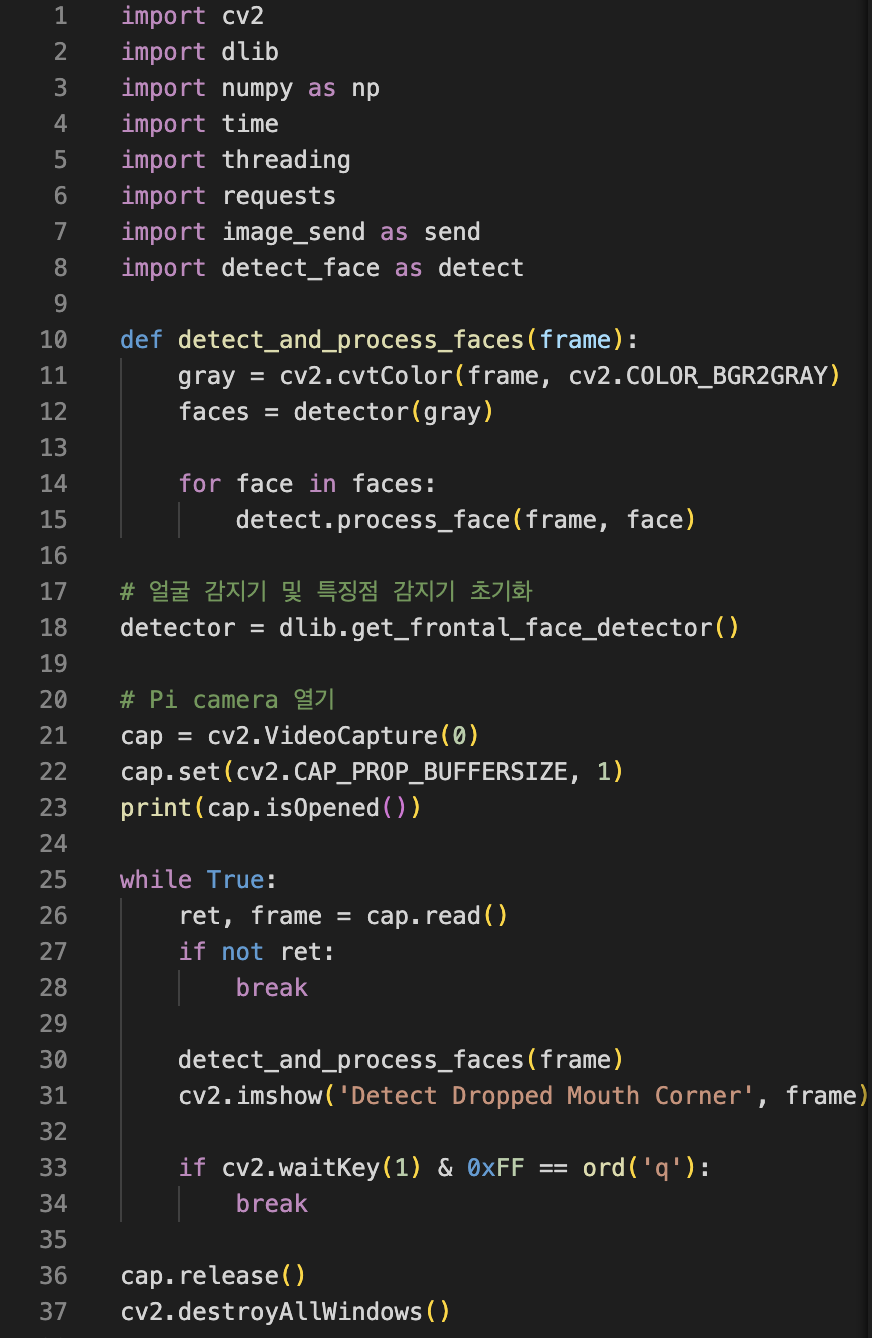
\includegraphics[width=0.5\linewidth]{images/first_level.png}
    \caption{first\_level.py}
    \label{fig:enter-label}
\end{figure}

\textbf{first\_level.py}
% main이 되는 실행파일로 OpenCV 라이브러리를 통해 camera로 부터 Video Stream 정보를 가져온다. 라즈베리파이의 하드웨어적 한계로 인해 Buffer size를 최소화여 Video Stream를 불러와야 한다. 이후 cv2.imshow를 통해 처리된 video stream을 볼 수 있다. 또한 first_level.py에서 처리되는 정보를 Gray scale로 변경해준다. Gray Scale을 사용하는 이유는 첫 째, 정보의 용량이 감소한다. RGB를 사용할 경우 RGB 3개의 색상 channel이 생기므로 처리할 정보가 늘어난다. 본 프로젝트에서는 색상 정보가 필요하지 않기때문에 gray scale로 변경해 용량을 줄이고 처리 속도를 향상시키고자 하였다. 둘 째, 노이즈가 감소한다. IoT 장비에 들어가는 카메라는 고성능일 수 없다. 따라서 화질이 안좋은 만큼 노이즈가 많을텐데 gray scale로 변경함으로써 노이즈를 줄이고 우리가 원하는 drooping 정보를 깔끔하게 얻을 수 있다. gray scale로 변경하는 작업은 픽셀을 하나씩 변경해주어야하는데 OpenCV에서 cv2.cvtColor 함수를 제공하기에 이를 사용해서 simple하게 바꿀 수 있다. 또한 face landmark 탐지를 위해 dlib 함수를 사용해 gray scale로 변경된 Video stream을 이 함수에 전달해주는 것까지 해당 파일에서 진행한다.

The main executable file uses the OpenCV library to capture video stream information from the camera. Due to hardware limitations of the Raspberry Pi, it is essential to minimize the buffer size for loading the video stream. Subsequently, the processed video stream can be viewed using cv2.imshow. Additionally, the information processed in first\_level.py is converted to grayscale. The rationale behind using grayscale is twofold. Firstly, it reduces the data size since using RGB would introduce three color channels, increasing the processing load. As color information is unnecessary for this project, converting to grayscale reduces the data size, enhancing processing speed. Secondly, it decreases noise. Cameras for IoT devices may not be high-performance, resulting in potentially noisy images. Converting to grayscale helps mitigate noise, allowing us to obtain clean drooping information. The task of converting to grayscale involves altering each pixel, a task facilitated by the cv2.cvtColor function in OpenCV. Furthermore, in the same file, the video stream, now in grayscale, is passed to the dlib function for face landmark detection.\\

\begin{figure}[h]
    \centering
    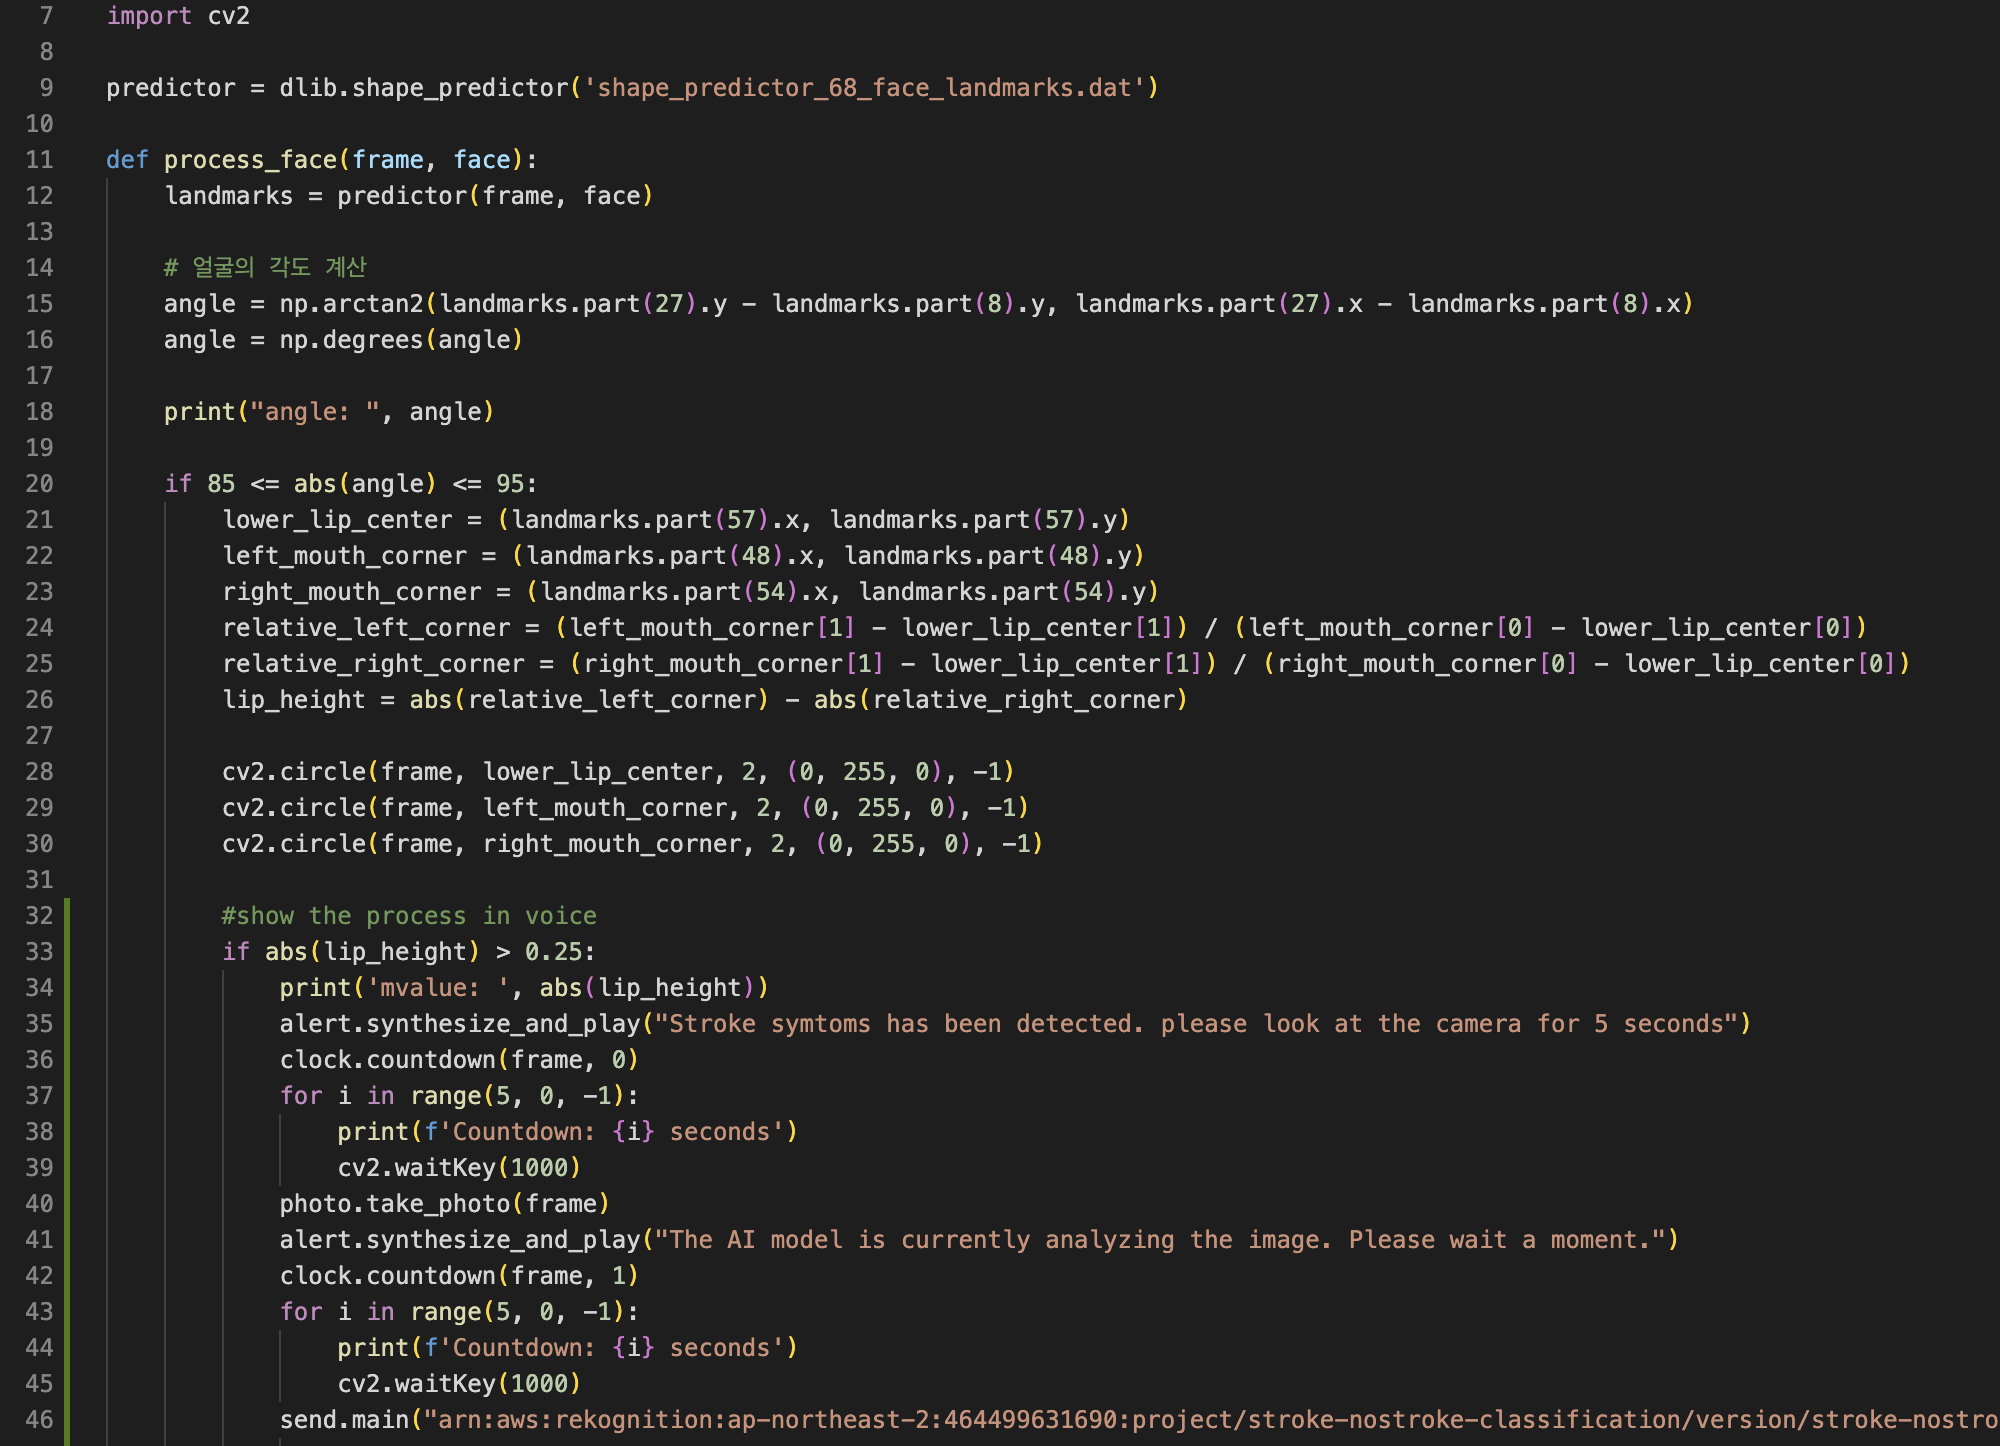
\includegraphics[width=0.5\linewidth]{images/detect_face.png}
    \caption{detect\_face.py}
    \label{fig:enter-label}
\end{figure}

\textbf{detect\_face.py}
%detect_face에서는 m-value를 계산하여 first detection을 수행한다. 또한 Video Stream을 처리하기 때문에 과하게 얼굴 각도가 기울어져있으면 결과에 영향을 주기도 한다. 그래서 먼저 얼굴 각도를 계산한다. landmark의 27번 인덱스와 8번 인덱스는 얼굴의 상하단 좌표이다. numpy의 arctan함수를 사용해 각도를 구하고 이 각도가 85도에서 95도 사이일 경우에만 first_level detection이 진행된다. 이후 m-value를 구한다. landmark의 57번 인덱스는 아랫입술의 가운데 좌표이고, 48번은 왼쪽 끝, 54번은 오른쪽 끝 좌표이다. 아랫입술과 양쪽 입술 끝의 차이를 relative_corner로 구하며 이 차이가 곧 m_value가 된다. 이 m_value가 0.25 이상일 경우에 first_level detection에 잡히게 되고 이후 second_level detection을 위한 사진을 촬영한다. 동시에 이를 aws polly를 이용해 voice로 알림을 준다. 추가로 frame에서의 입술의 좌표를 보여주는 것과 face landmark를 위한 dlib의 보조 파일을 주는 것까지 detect_face.py에서 수행한다.

In the detect\_face module, the m\_value is computed to perform the initial detection. Given that it processes a video stream, excessively tilted face angles can impact the results. Therefore, the first step involves calculating the face angle. Landmark indices 27 and 8 represent the top and bottom coordinates of the face. Using the arctan function of numpy, the angle is computed, and first-level detection proceeds only when this angle between 85 and 95 degrees. After that, the m-value is determined. Landmark index 57 corresponds to the center coordinate of the lower lip, while 48 and 54 represent the left and right ends, respectively. The difference between the lower lip and the ends of both lips, known as relative\_corner, becomes the m-value. If this m\_value is greater than or equal to 0.25, it triggers the first-level detection, capturing a photo for subsequent second\_level detection. Simultaneously, an alert is provided using AWS Polly in a voice format. Additionally, detect\_face.py handles displaying lip coordinates on the frame and providing auxiliary files for face landmarks using dlib.\\

\begin{figure}[h]
    \centering
    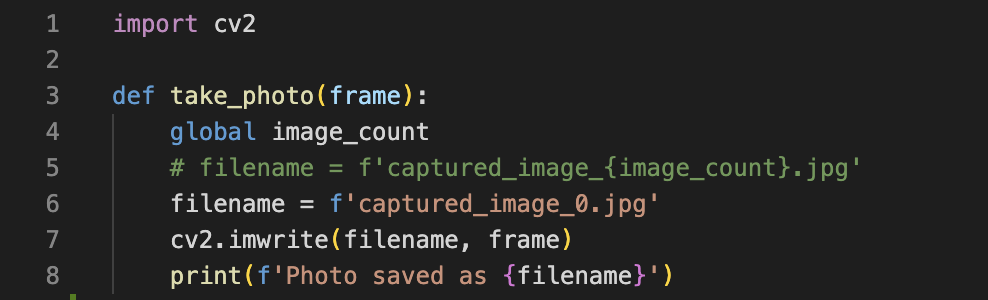
\includegraphics[width=0.5\linewidth]{images/take_photo.png}
    \caption{take\_photo.py}
    \label{fig:enter-label}
\end{figure}

\textbf{take\_photo.py}
%take_photo.py는 second_level detection으로 전송할 사진을 찍는 기능을 수행한다. openCV의 imwrite 함수를 활용해 현재 frame에 잡혀있는 모습을 이미지로 저장한다. IoT에 들어갈 소프트웨어이기 때문에 찍은 사진을 전부 저장하지 않고 가장 최근에 찍은 사진만을 local에 저장한다. 이전 이미지들은 second_level로 전송됨과 동시에 aws cloud에 저장된다. 

The take\_photo.py module serves the functionality of capturing a photo to be sent for second-level detection. It utilizes the imwrite function from OpenCV to save the current frame as an image. Given its purpose as software for IoT, it only retains the most recently captured photo locally, instead of storing all the taken pictures. Previous images are sent for second\_level detection and concurrently stored in the AWS Cloud.\\

\begin{figure}[h]
    \centering
    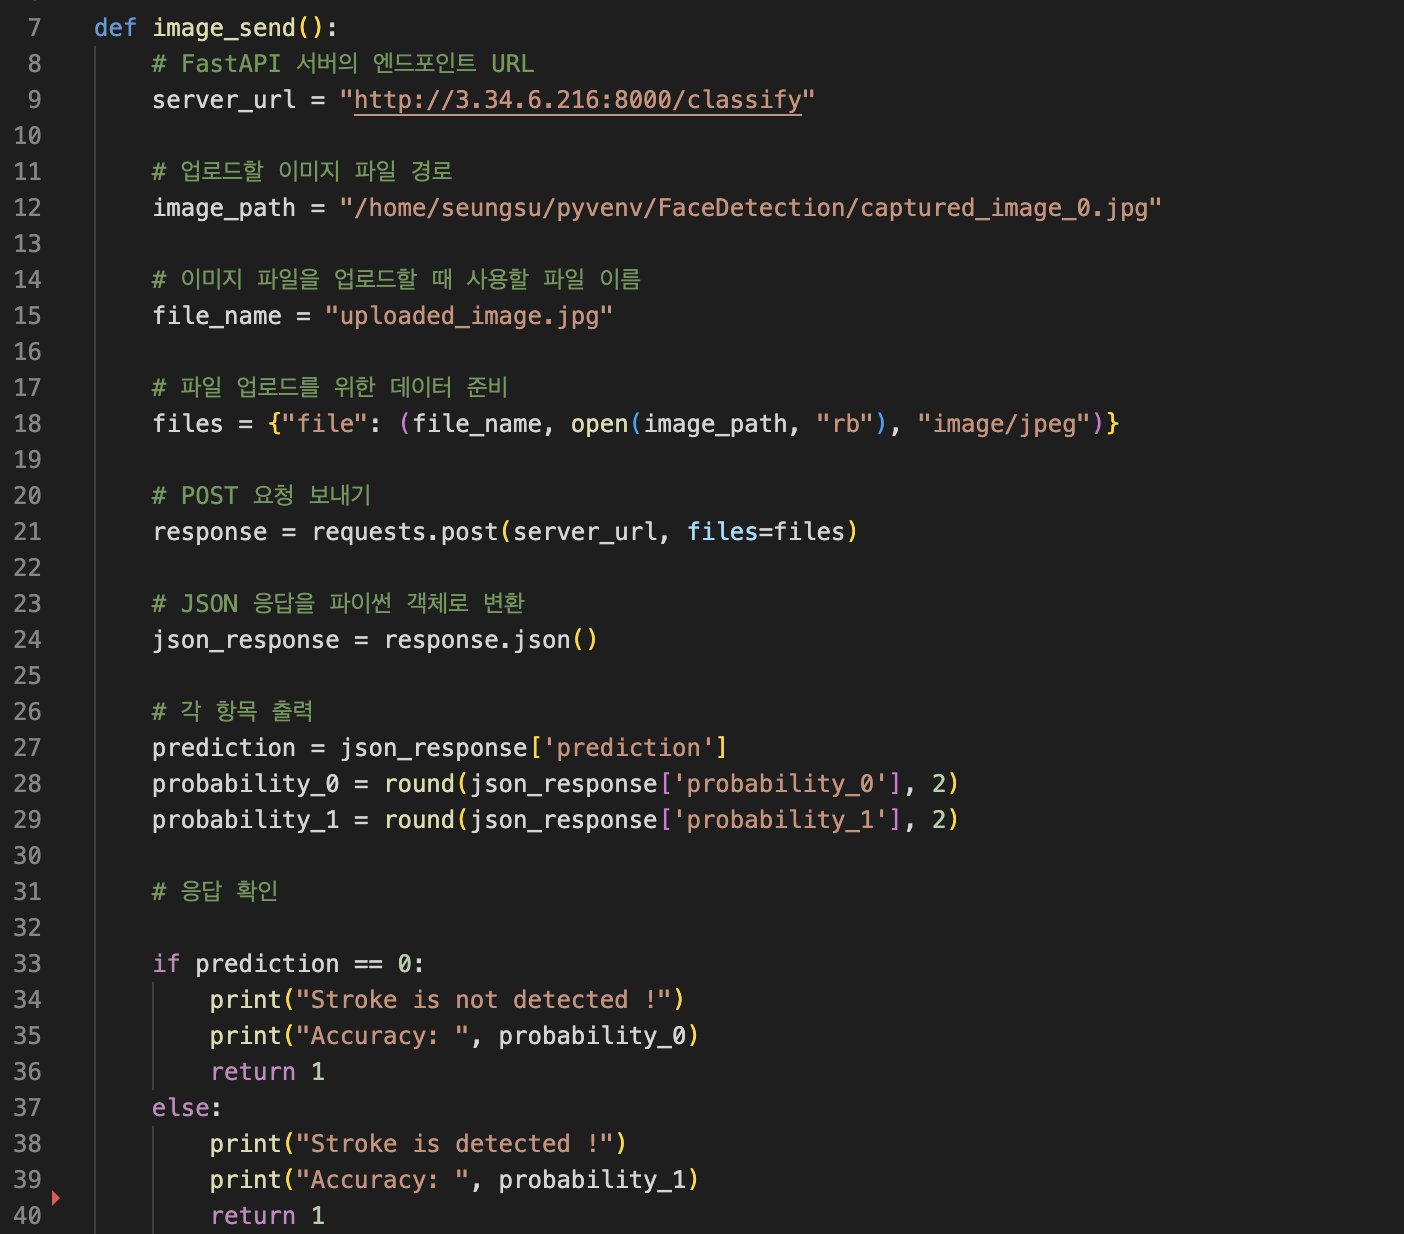
\includegraphics[width=0.5\linewidth]{images/image_send.png}
    \caption{image\_send.py}
    \label{fig:enter-label}
\end{figure}

\textbf{image\_send.py}
%image_send.py는 웹서버를 통해 second_level detection을 진행할 때 사용된다. 실행중인 웹서버의 url을 가지고 특정 이미지 파일을 전송한다. POST방식을 사용해 request를 보내고 json 파일로 response를 받는다. 이후 response된 json파일을 python 객체로 변환한 후 response의 인덱스에 따른 결과값을 확인한다. prediction이 0이라면 stroke이 탐지되지 않은 것이고 이외의 값이라면 탐지된 것이다. 이때 second_level model이 판단한 Accuracy까지 user에게 보여준다.

The image\_send.py module is used when going second-level detection through a web server. It sends a specific image file to the running web server's URL using the POST method, then receives the response in the form of a JSON. Subsequently, it converts the received JSON file into a Python object and checks the result based on the response index. If the prediction is 0, it indicates that a stroke has not been detected; otherwise, it signifies a detection. Additionally, it displays the accuracy determined by the second-level model to the user.\\

\begin{figure}[h]
    \centering
    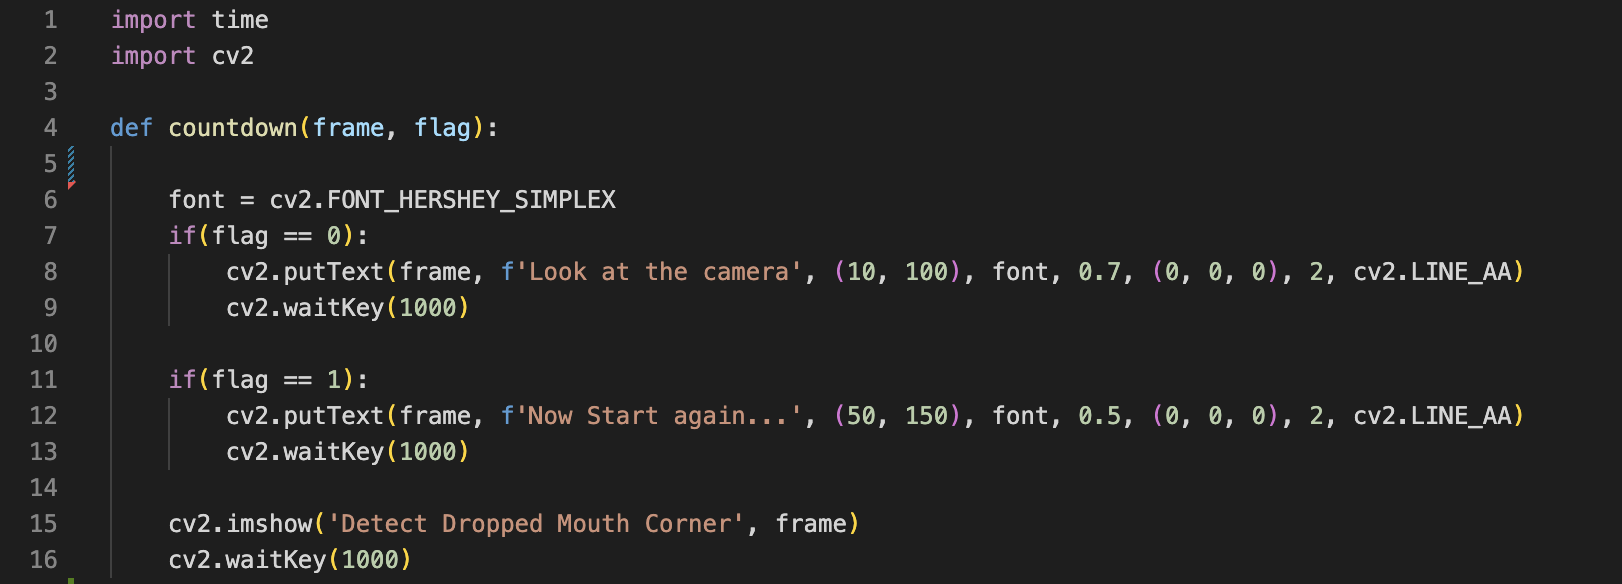
\includegraphics[width=0.5\linewidth]{images/count_clock.png}
    \caption{count\_clock.py}
    \label{fig:enter-label}
\end{figure}

\textbf{count\_clock.py}
%count\_clock.py는 openCV imshow frame에 카운트를 띄우는 기능을 한다. first_level에서 Mouse drooping이 발견되면 사진을 찍기 전 "Look at the camera"를, 사진을 찍은 후엔 다시 first_level로 돌아가기 전까지 "Now Start again..."을 보여준다.

The count\_clock.py module performs the function of displaying a count on the OpenCV imshow frame. When Mouse drooping is detected in the first\_level, it shows "Look at the camera" before taking a photo, and after capturing the photo, it displays "Now Start again..." until returning to the first\_level.\\

\begin{figure}[h]
  \centering
  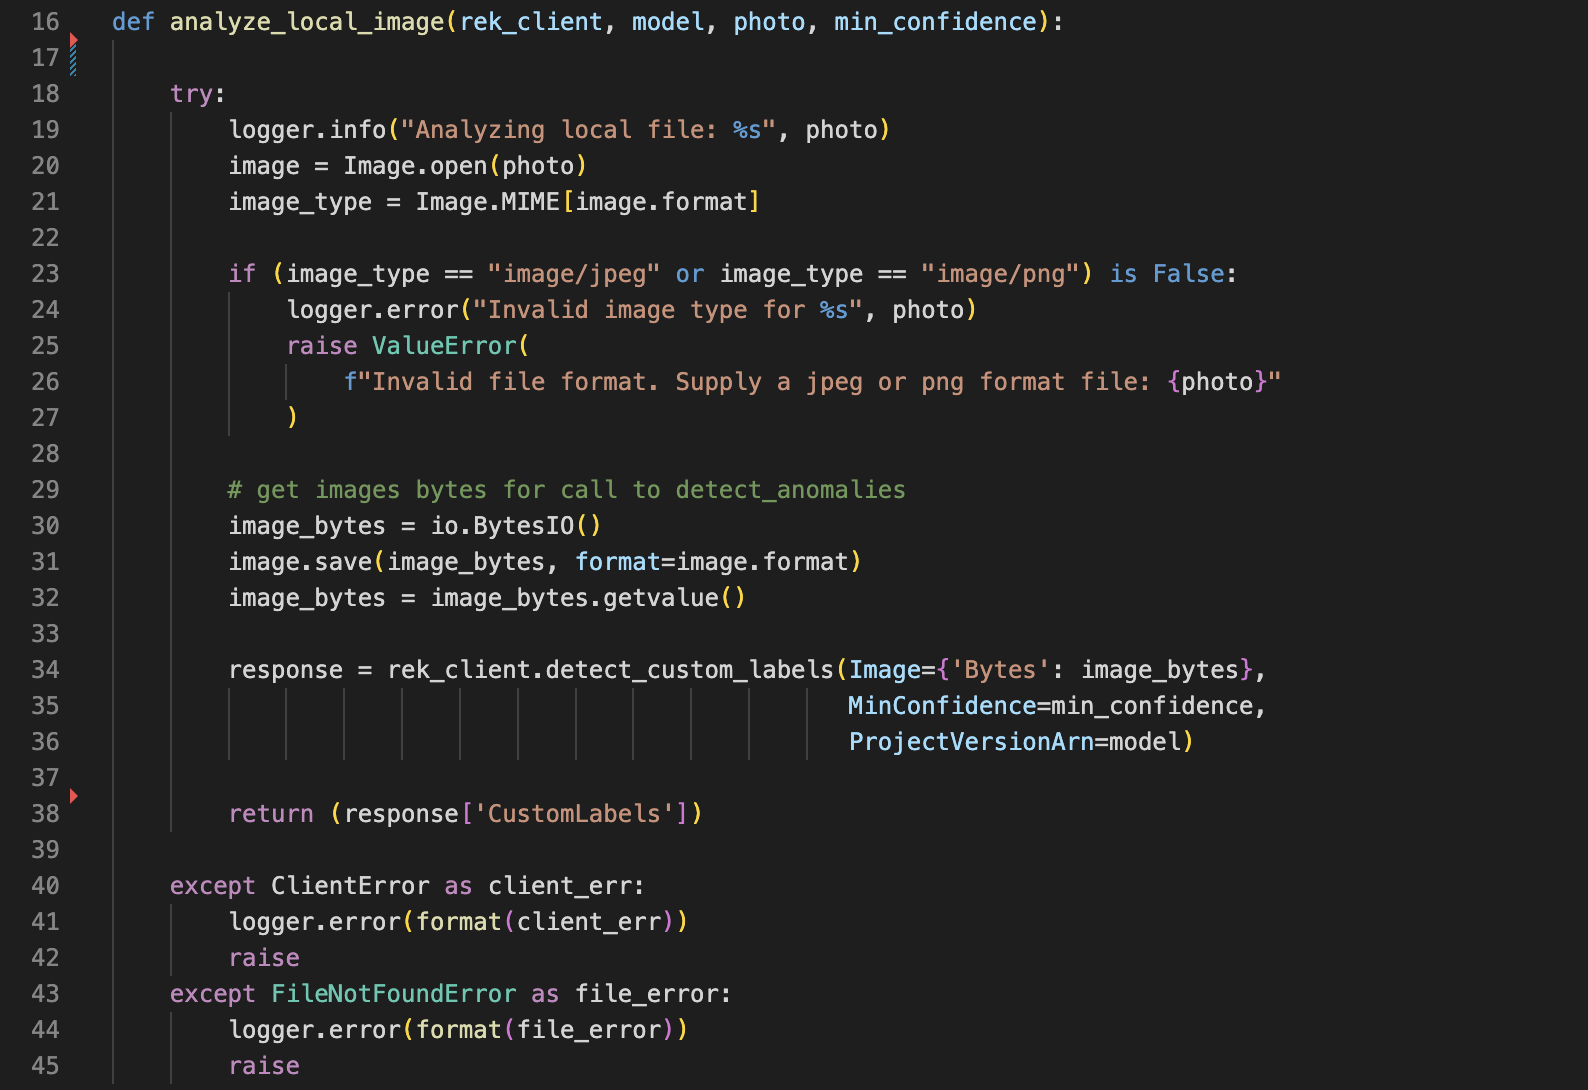
\includegraphics[width=0.45\textwidth]{images/send_aws_1.png}
  \hspace{0.05\textwidth}
  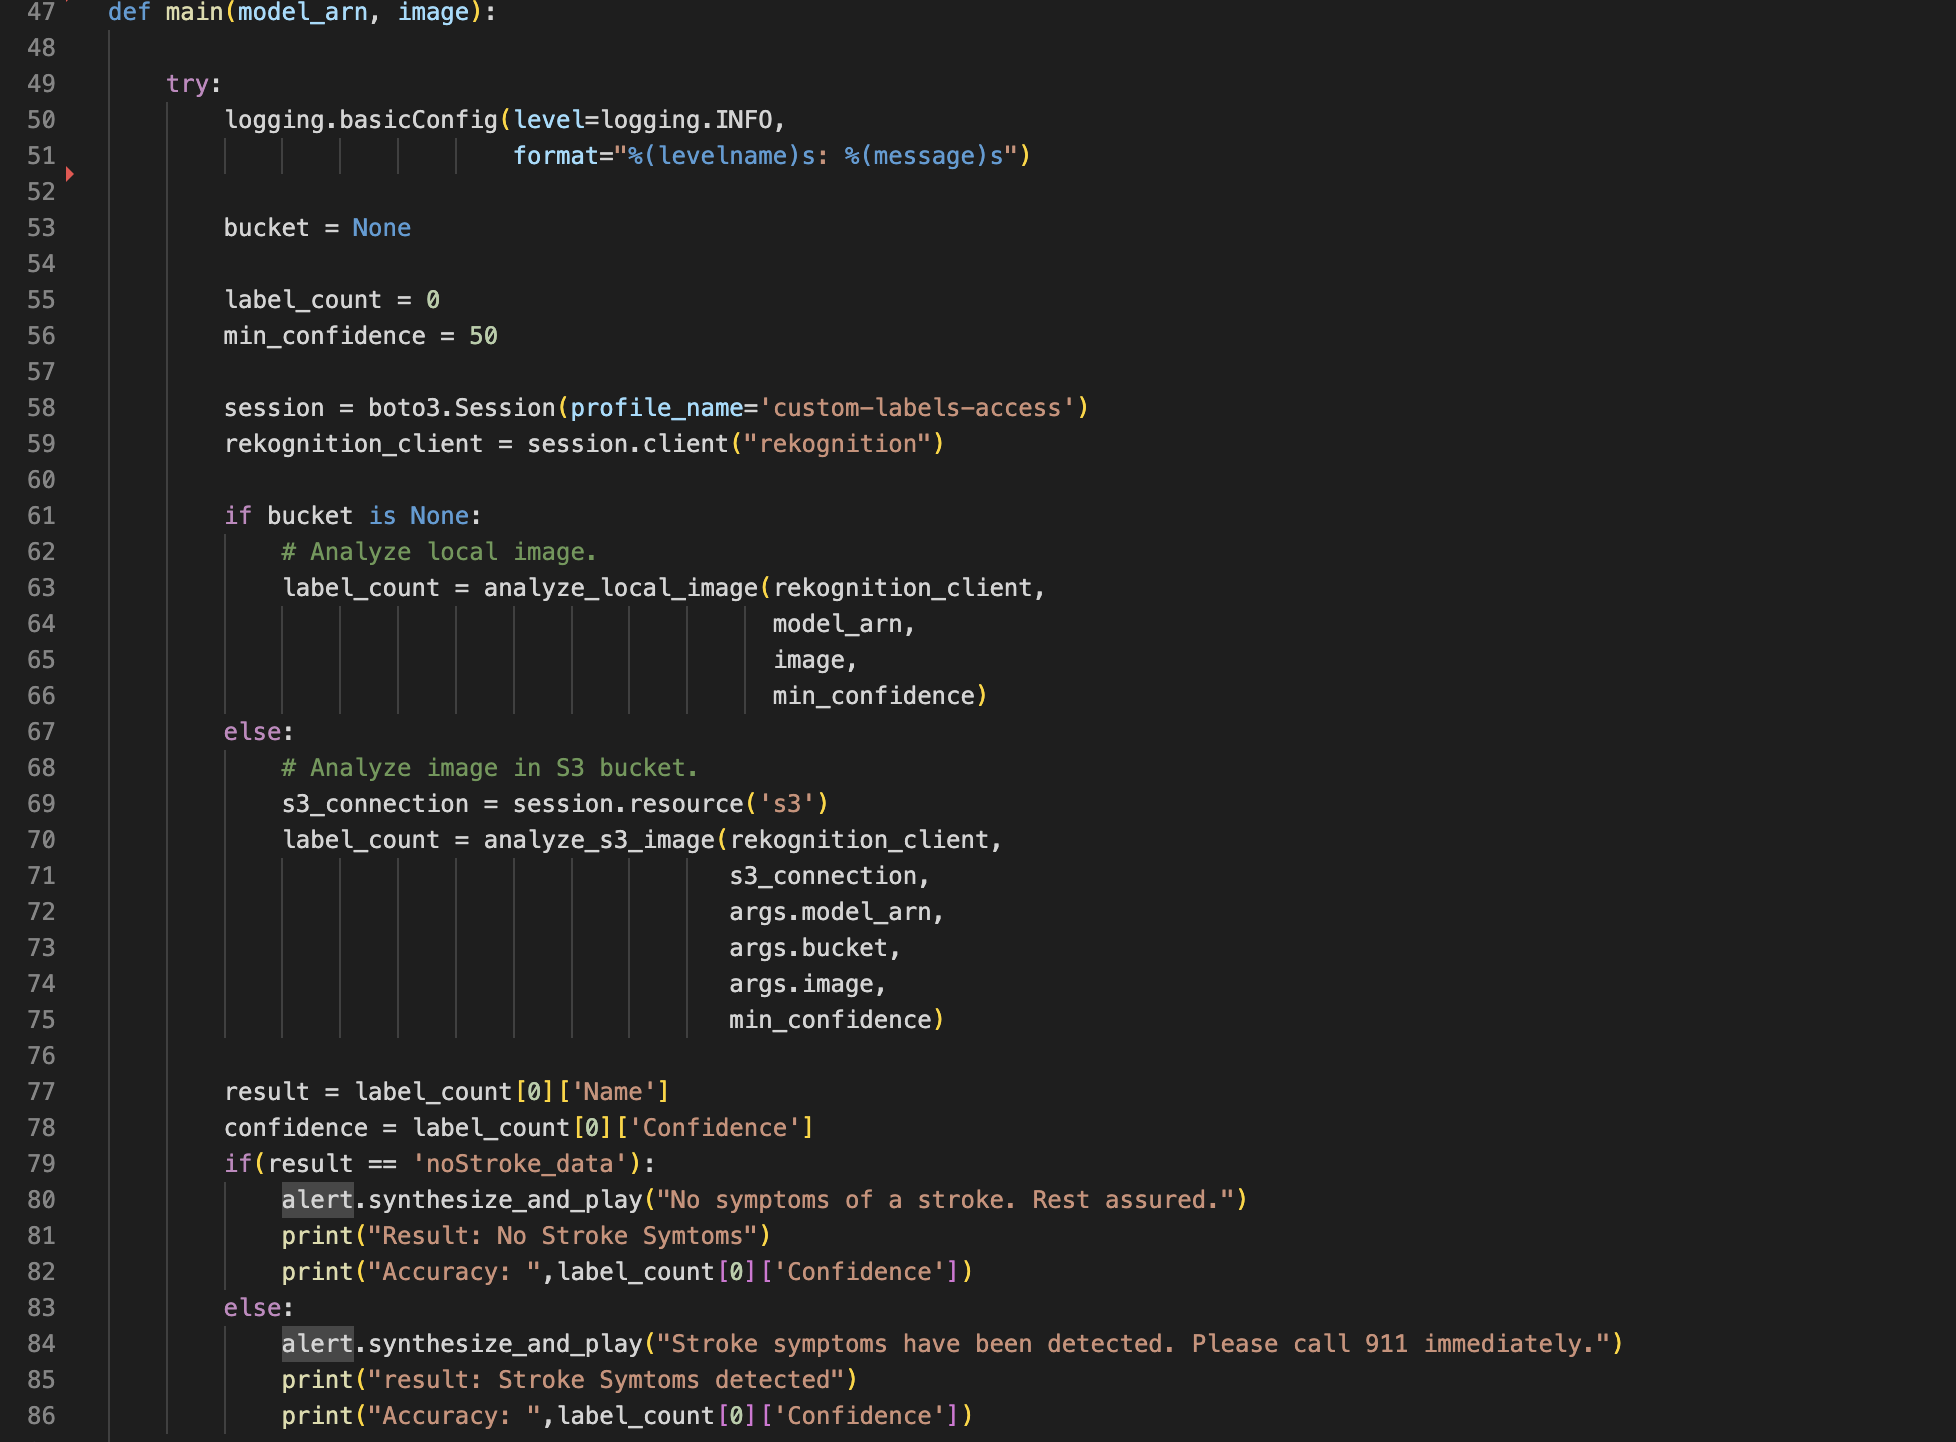
\includegraphics[width=0.45\textwidth]{images/send_aws_2.png}
  \caption{send\_aws.py}
  \label{fig:twopics}
\end{figure}

\textbf{send\_aws.py}
This script utilizes the AWS Rekognition service to detect custom labels in images and generate voice alerts based on the detected labels. The code reads an image from a local file, uses the Amazon Rekognition Custom Labels to detect labels defined in a custom model, and triggers voice alerts accordingly.

Key functions and components:
\begin{enumerate}
    \item analyze\_local\_image: 
    This function reads an image from a local file, uses Amazon Rekognition Custom Labels to detect labels in the user-defined model, and returns the detected labels.\\
    \item main: 
    The main function of the script takes the model ARN and image path as input, analyzes the image, and generates a voice alert based on the results.\\
    \item The code interacts with AWS services using the Boto3 AWS SDK. It sets up a session with boto3.Session and communicates with the Rekognition service through the rekognition\_client.
    \item Voice alerts are generated using the voice\_alert module, specifically the synthesize\_and\_play function, which synthesizes text into speech and plays it.\\
    \item Error handling is implemented to appropriately handle exceptions, and logging is used to output information and error messages.\\
    \item The section if \_\_name\_\_ == "\_\_main\_\_": is the typical entry point for a Python script, ensuring that the main function is called only when the script is executed directly.\\
\end{enumerate}
This code primarily focuses on utilizing the AWS Rekognition service for image processing and custom label detection, demonstrating the functionality of an application that triggers voice alerts based on image analysis results.\\

\begin{figure}[h]
  \centering
  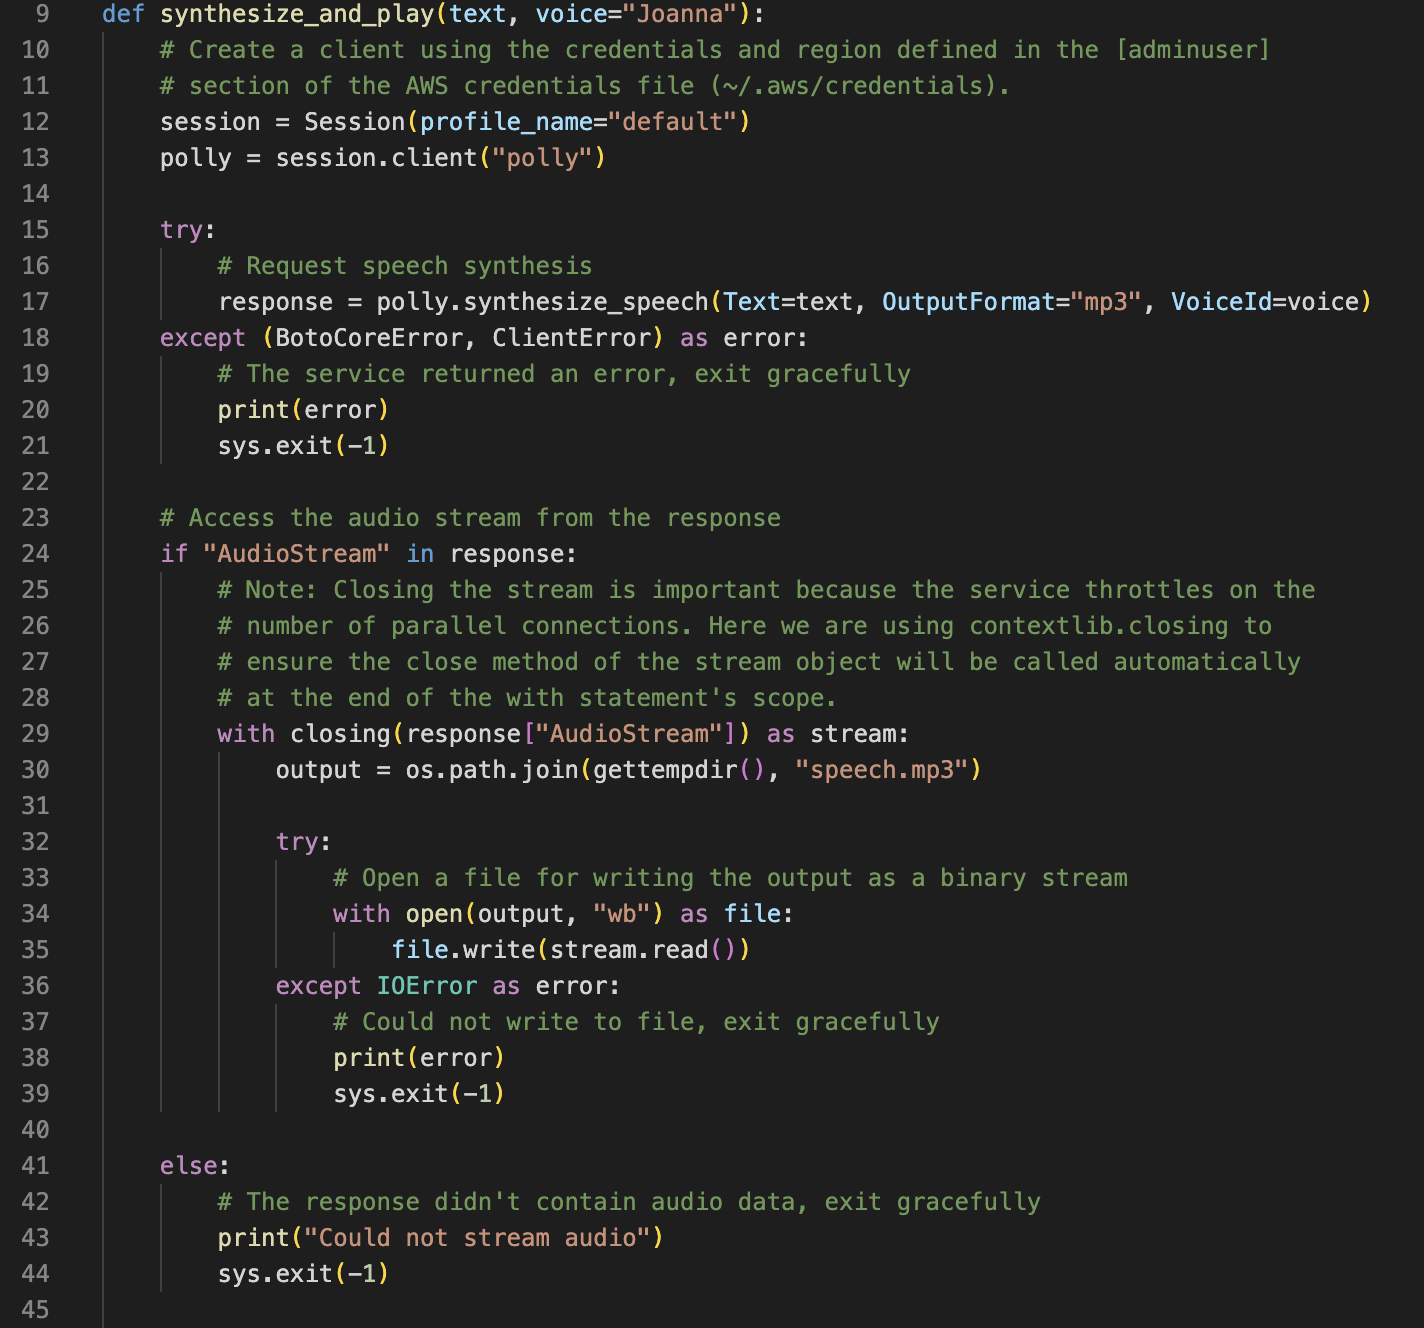
\includegraphics[width=0.45\textwidth]{images/voice_alert_1.png}
  \hspace{0.05\textwidth}
  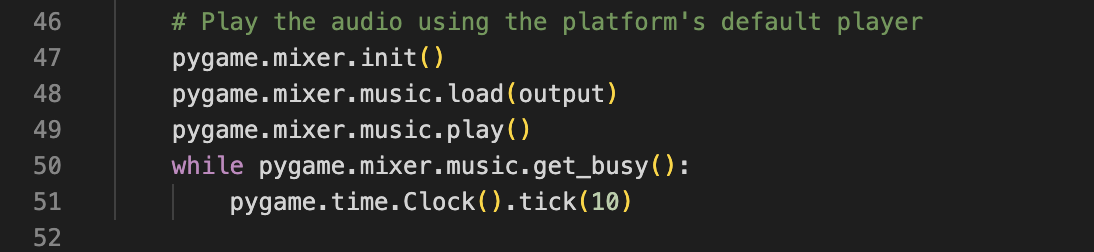
\includegraphics[width=0.45\textwidth]{images/voice_alert_2.png}
  \caption{alert\_aws.py}
  \label{fig:twopics}
\end{figure}

\textbf{voice\_alert.py}
This is designed to synthesize speech from a given text using the Amazon Polly service and play the resulting audio.

\begin{enumerate}
    \item Input Parameters:
    text: The input text that needs to be synthesized into speech.
    voice (optional, default is "Joanna"): The voice to be used for speech synthesis.
    \item Function Steps:
    It creates an AWS Polly client using the AWS credentials and region defined in the [default] section of the AWS credentials file (~/.aws/credentials).
    Attempts to synthesize speech by making a request to Polly with the provided text, specifying the desired output format ("mp3") and voice.
    Handles potential errors such as BotoCoreError or ClientError that may occur during the Polly service request. If an error occurs, it prints the error message and exits the script with an error code (-1).
    If the response from Polly contains an audio stream ("AudioStream"), it saves the audio stream to a temporary mp3 file on the local system.
    If there is an issue with streaming audio or writing to a file, it exits gracefully, printing an error message.
    Finally, it uses the Pygame library to play the synthesized speech using the platform's default audio player. It ensures that the program doesn't exit until the audio has finished playing.
    \item Dependencies:
    The function depends on the boto3 library for AWS interaction and the pygame library for audio playback.
    \item Note:
    Make sure to have the necessary AWS credentials configured on the system.
\end{enumerate}

The script expects Pygame to be installed for audio playback.
Overall, this function provides a convenient way to synthesize speech from text using Amazon Polly and play the generated audio using the Pygame library.

\begin{figure}[h]
    \centering
    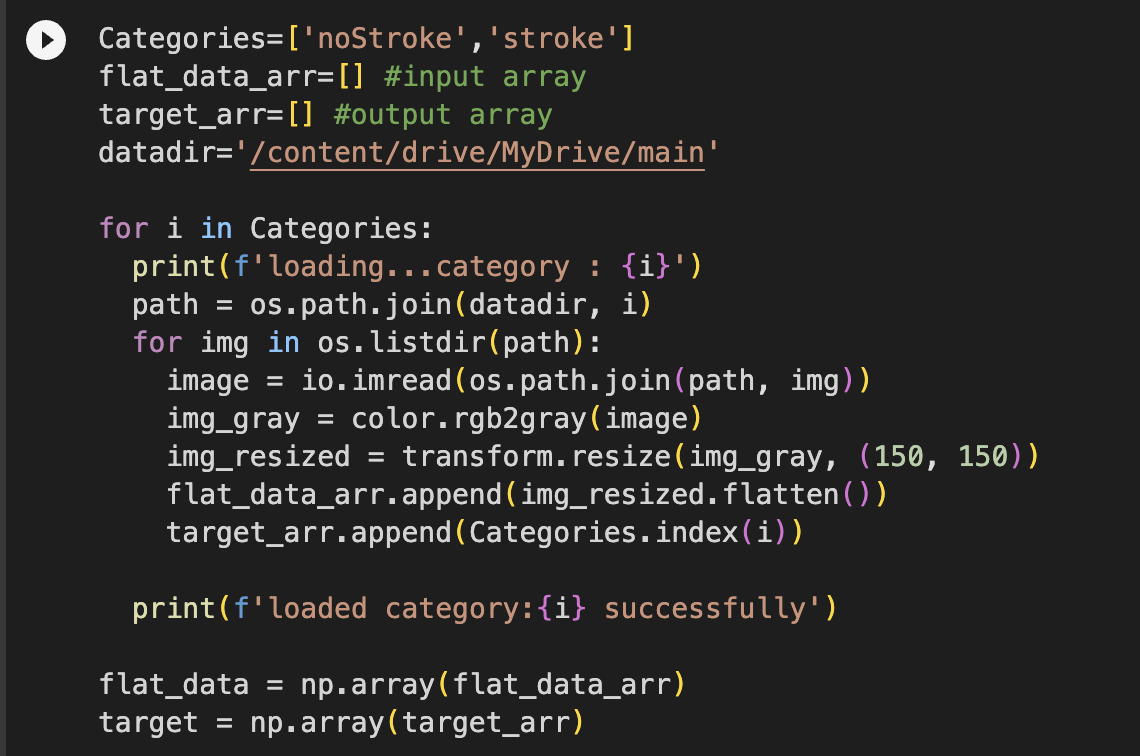
\includegraphics[width=8.5cm]{images/rf_data.png}
    \caption{Pre-processing data in Random Forest}
    \label{fig:enter-label}
\end{figure}

\subsubsection{Module2: AI-back}
% AI-back 모듈은 2-Level detection에서 2단계를 구성하는 요소이다. 인공지능 모델로 3가지를 생각했다. 머신러닝 기반의 Support Vector Machine과 앙상블 학습을 하는 Random Forest, 그리고 딥러닝 기반의 ViT를 각각 만들고 실험했다. ipynb 파일은 Google Colab에서 작성한 코드이다.
The AI-back module is an element that constitutes the second stage in 2-Level detection. We thought of three things as an artificial intelligence model. We created and tested machine learning based Support Vector Machine, random forest using ensemble learning, and deep learning-based ViT. The ipynb file is code written in Google Colab.

\textbf{SE\_RandomForest.ipynb} \\
% Random Forest 머신러닝 모델을 사용하고 그 모델을 훈련시키는 노트북 파일이다. 파일은 크게 3부분으로 나뉜다. 첫째, 뇌졸중 환자와 정상인의 얼굴 데이터를 불러와서 전처리를 하는 과정. 둘째, 전처리한 데이터를 랜덤 포레스트 모델을 불러와서 학습시키는 과정. 마지막으로 훈련을 마친 모델을 테스트하는 과정이다.
This is a notebook file that uses the Random Forest machine learning model and trains the model. The file is divided into three parts. First, the process of loading and pre-processing face data of stroke patients and normal people. Second, the process of loading and training the random forest model on the preprocessed data. Lastly, it is the process of testing the trained model.

% 데이터 전처리는 다음과 같은 과정으로 이루어진다. 이미지를 폴더에서 불러오고 흑백으로 전환한다. 이미지의 색깔과 표정은 독립적이므로 입력의 차원값을 줄이는 방향으로 진행했다. 이미지 데이터의 크기가 제각각이므로 (150, 150)의 크기로 변환하고 이를 평면화해서 벡터로 만들었다. 
Data preprocessing consists of the following processes. Load an image from a folder and convert it to black and white. Since the color and expression of the image are independent, we proceeded to reduce the dimension of the input. Since the size of the image data is different, we converted it to a size of (150, 150) and flattened it into a vector.

\begin{figure}[h]
    \centering
    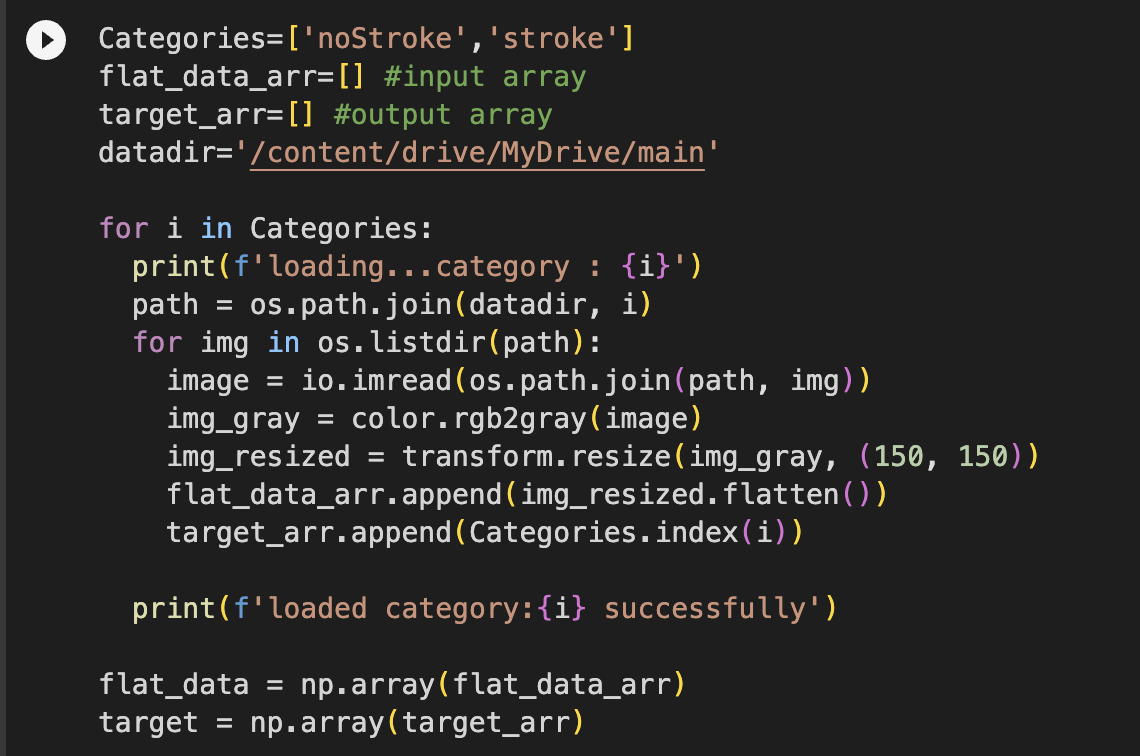
\includegraphics[width=8.5cm]{images/rf_data.png}
    \caption{Pre-processing data in Random Forest}
    \label{fig:enter-label}
\end{figure}

% 사이킷런의 라이브러리를 활용해 모델을 import했다. 훈련용 데이터와 테스트용 데이터를 80%, 20%로 나누고 훈련용 데이터로 학습시켰다. 이 과정은 수분밖에 소요되지 않았다.
The model was imported using scikit-learn’s library. The training data and testing data were divided into 80\% and 20\% and learned using the training data. This process took only a few minutes.

% 마지막으로 학습이 완료된 모델을 테스트 데이터로 검증한다. 이때, 단순한 정확도로는 뇌졸중 판단 모델의 성능을 확실시 할 수 없다. 사람의 건강을 판단하는 것이기 때문에 true positive, false negative 등 자세하게 판단해야 한다. classification_report 함수를 사용해서 더 정확한 성능을 판단한다.
Finally, the trained model is verified with test data. At this time, the performance of the stroke judgment model cannot be assured with simple accuracy. Since it is a judgment of a person's health, it must be judged in detail, including true positives and false negatives. Use the classification\_report function to determine more accurate performance.

% 아래는 실제 classification_report 함수를 적용한 결과이다. 주목해야 할 점은 stroke의 precision 값이 0.97로 매우 높다는 점이다. 이는 모델이 stroke라 판단했으면 실제로 stroke인 확률이 97%인 것이다. 반면 stroke recall은 0.72로 떨어지는데 이는 실제로는 stroke이지만 stroke로 모델이 판단을 하지 못한 것이 28%라는 뜻이다. 전체적으로 stroke의 정확도가 no-stroke 판단의 정화도보다 낮은데 이는 데이터의 갯수가 no-stroke가 많기 때문이라고 사료된다.
Below is the result of applying the actual classification\_report function. What is important to note is that the stroke precision value is very high at 0.97. This means that if the model determines that it is a stroke, there is a 97\% probability that it is actually a stroke. On the other hand, stroke recall drops to 0.72, which means that 28\% of cases were actually strokes, but the model failed to judge them as strokes. Overall, the accuracy of stroke is lower than the precision of no-stroke judgment, which is believed to be because the number of data is large.
\begin{figure}[h]
    \centering
    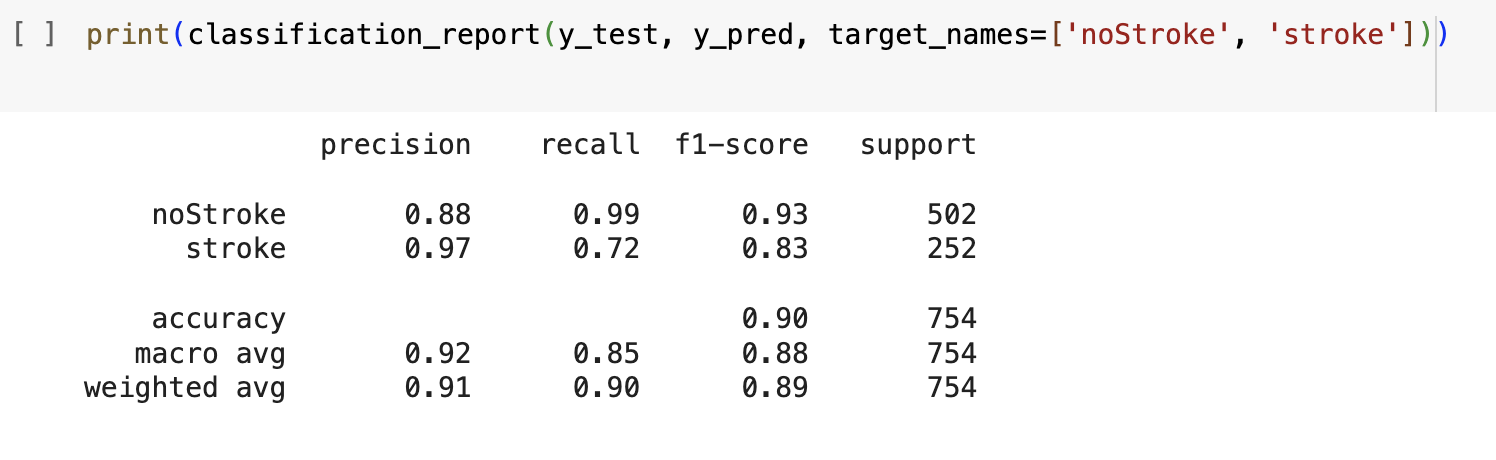
\includegraphics[width=8.5cm]{images/rf_result.png}
    \caption{The result of testing Random Forest model}
    \label{fig:enter-label}
\end{figure}


\textbf{rf\_stroke\_classification} \\
% 위의 파일로 훈련이 완료된 모델이다. joblib 함수로 파일을 저장했다. 이후 이 파일을 AWS Lightsail에 옮기고 후술될 app.py 파일에서 호출해서 웹 서버로 올린다. 이것으로 모델을 웹 서버로 배포한다.
This is a model that has been trained with the file above. The file was saved using the joblib function. Afterwards, move this file to AWS Lightsail and upload it to the web server by calling it from the app.py file, which will be described later. This deploys the model to the web server.

\textbf{SE\_SVM.ipynb} \\
% Support Vector Machine 기반으로 학습을 진행하는데 사용된 파일이다. Google Colab에서 작동했으며 SE\_RandomForest.ipynb 파일과 동일한 과정을 거쳐 데이터 전처리, 학습, 검증을 했다.
This is a file used to conduct learning based on Support Vector Machine. It ran in Google Colab and went through the same process as the SE\_RandomForest.ipynb file for data preprocessing, learning, and verification.

% 데이터 전처리는 이미지의 색을 흑백으로 전환해 데이터의 차원 수를 낮추고 크기를 (150, 150)으로 일괄적으로 변환했다. 이미지 전처리 과정에서 SE\_RandomForest.ipynb 파일과 차이점은 훈련 데이터의 갯수를 500개로 제한했다는 점이다. 똑같이 모든 데이터를 활용해서 훈련을 진행하면 Google Colab CPU로 훈련했을 때, 5시간 넘게 진행해도 훈련이 종료되지 않았다. 이렇게 모든 데이터를 훈련에 사용하는 것은 무리가 있다고 판단해 500개로 데이터의 개수를 제한해서 사용했다.
For data preprocessing, the color of the image was converted to black and white, the number of dimensions of the data was reduced, and the size was batch converted to (150, 150). The difference from the SE\_RandomForest.ipynb file in the image preprocessing process is that the number of training data is limited to 500. When training was performed using all data in the same way, when training was performed with Google Colab CPU, training did not end even after more than 5 hours. We judged that it would be unreasonable to use all the data for training, so we limited the number of data to 500.

\begin{figure}[h]
    \centering
    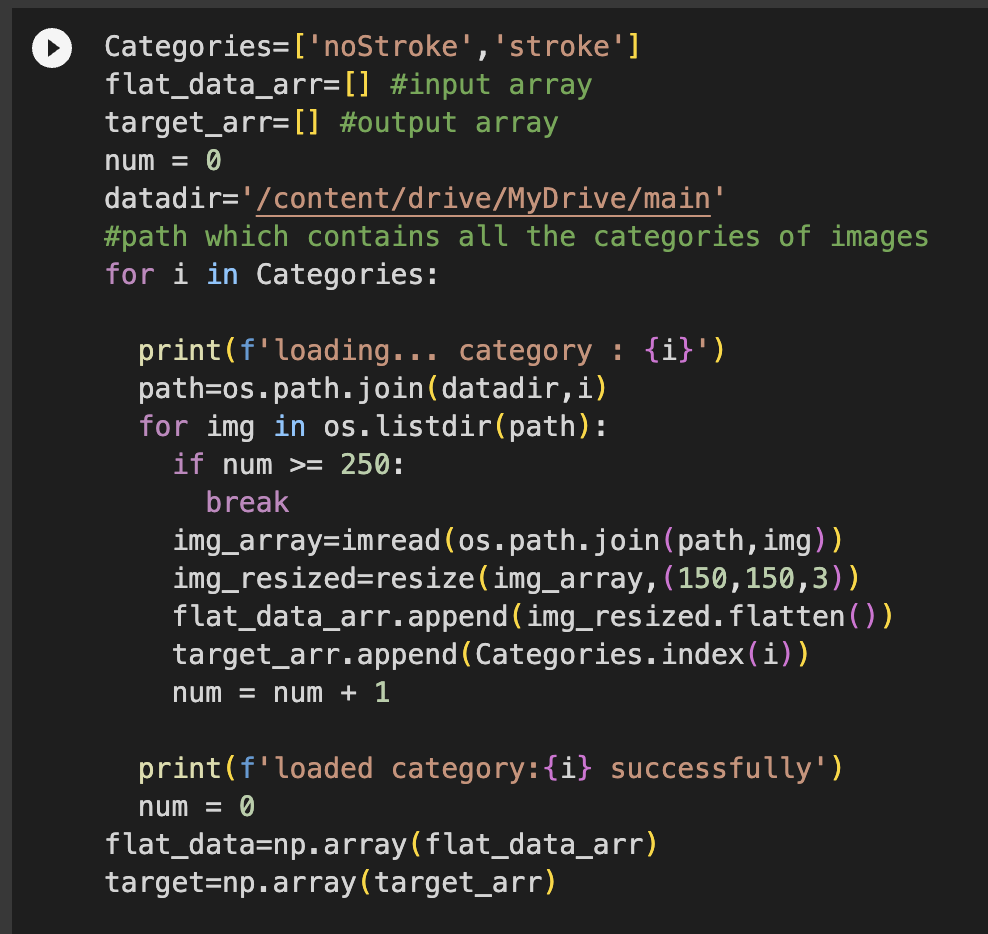
\includegraphics[width=8.5cm]{images/svm_data.png}
    \caption{Pre-processing data in Support Vector Machine}
    \label{fig:enter-label}
\end{figure}

% scikit-learn의 SVC를 불러와서 훈련을 진행했다. 훈련용 데이터와 테스트용 데이터는 위와 같이 각각 80%, 20%로 구성했으며 훈련 시간은 1시간 내외로 소요됐다.
Then, we loaded scikit-learn's SVC and ran training. The training time, which consists of 80\% training data and 20\% testing data, is approximately 1 hour.


% 테스트 검증 결과는 다음과 같다. 자세한 정확도를 구하기 위해 classification_report를 사용했고 모든 경우에서 88%의 정확도를 보였다. 하지만 테스트 데이터의 양이 50개로 매우 적어서 유의미한 결과라고 해석하기는 어려웠고, 학습도 어려움이 있어 여기서 다른 모델을 강구하기 시작했다.
The test verification results are as follows. We used classification\_report to obtain detailed accuracy and showed an accuracy of 88\% in all cases. However, the amount of test data was very small at 50, so it was difficult to interpret the results as meaningful, and learning was also difficult, so we started looking for a different model.

\begin{figure}[h]
    \centering
    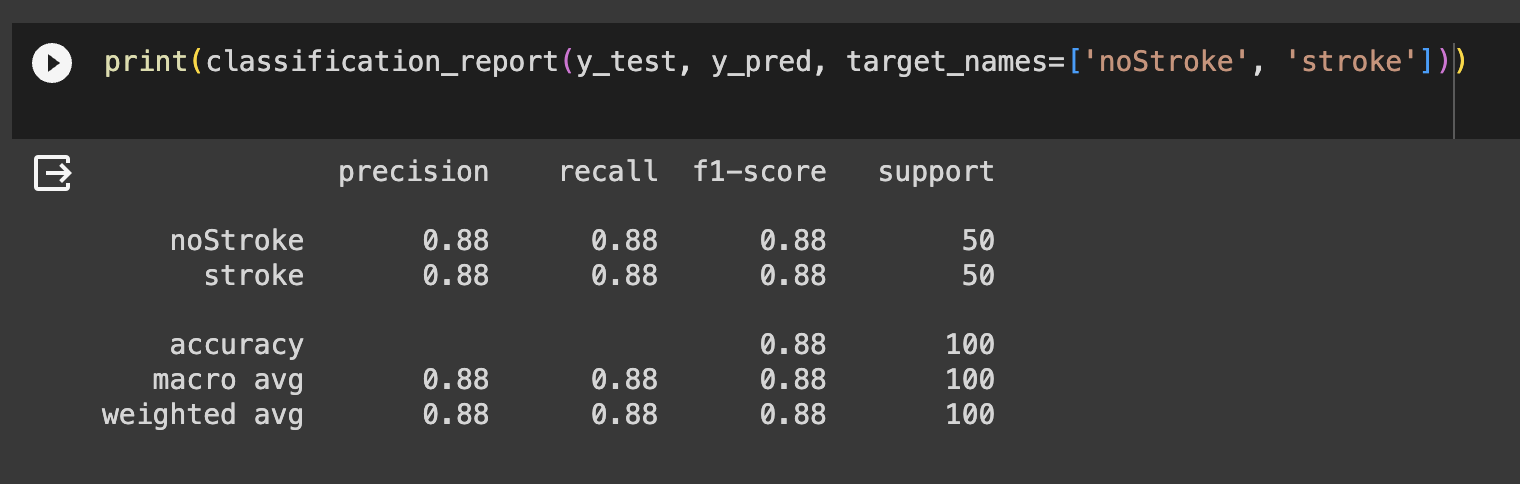
\includegraphics[width=8.5cm]{images/svm_result.png}
    \caption{The result of Support Vector Machine model}
    \label{fig:enter-label}
\end{figure}


% joblib 함수로 학습이 완료된 모델을 저장하고 AWS Lightsail로 옮겨 웹 서버로 배포했다. 이 때, 모델의 크기가 200MB를 넘었다. 이 점 또한 다른 모델을 찾아보기 시작한 이유 중 하나이다.
We saved the trained model using the joblib function, moved it to AWS Lightsail, and deployed it to a web server. At this time, the size of the model exceeded 200MB. This is also one of the reasons why I started looking for other models.

\begin{figure}[h]
    \centering
    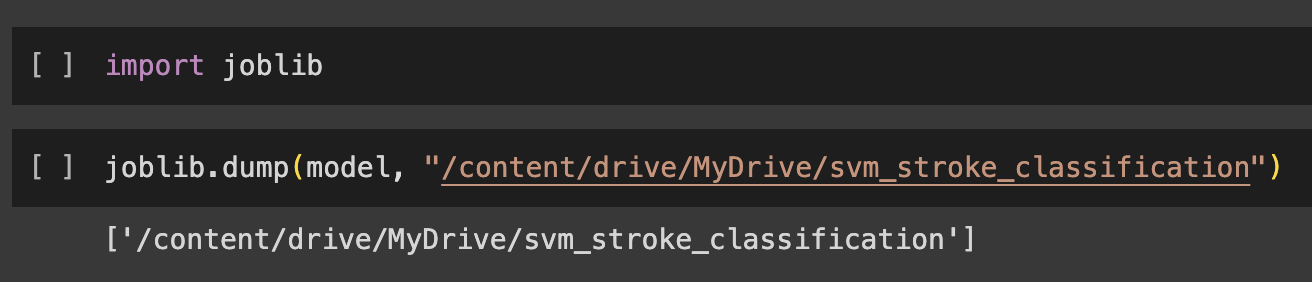
\includegraphics[width=8.5cm]{images/svm_save.png}
    \caption{Saving trained SVM model by using joblib}
    \label{fig:enter-label}
\end{figure}


\textbf{se\_svm.py} \\
% 위의 SE\_SVM.ipynb 파일을 python 파일 형식으로 저장한 것이다. 코드 파일의 내용은 위의 SE\_SVM.ipynb 와 같다.
The above SE\_SVM.ipynb file is saved in python file format. The contents of the code file are the same as SE\_SVM.ipynb above.


\textbf{SE\_ViT.ipynb} \\
% 이 파일은 ViT를 구현한 파일이다. ViT는 여러 모듈로 이루어진다. 이미지를 인식하기 위해 flatten시키는 patchify 모듈, patchify된 데이터에 원래 이미지에서의 위치 정보를 이식하는 positional_embedding 모듈, ViT에서 가장 중요한 작업인 Multi-head self attention을 수행하는 MSA 모듈, 이 모듈을 조립해 ViT class를 만들어서 구현을 완료한다. 
This file is a file that implements ViT. ViT consists of several modules. The patchify module that flattens the image for recognition, the positional\_embedding module that implants the positional information from the original image into the patchified data, and the MSA module that performs multi-head self attention, the most important task in ViT. These modules are assembled into a ViT class. Complete the implementation by creating.

% 학습에 필요한 데이터는 아래와 같이 전처리했다. pytorch 기반으로 ViT를 구현했으므로 Dataset과 이를 iteration할 수 있는 Dataloader를 직접 구현했다. 일관성을 유지하기 위해 흑백 사진으로 변환하고 이미지의 크기를 (150, 150)으로 바꾸었다. 사용한 함수는 다르지만 문맥은 위의 머신러닝 기반 모델과 동일하다.
The data needed for learning was preprocessed as follows. Since ViT was implemented based on pytorch, we directly implemented Dataset and Dataloader that can iterate on it. For consistency, I converted it to a black and white photo and resized the image to (150, 150). The functions used are different, but the context is the same as the machine learning-based model above.

\begin{figure}[h]
    \centering
    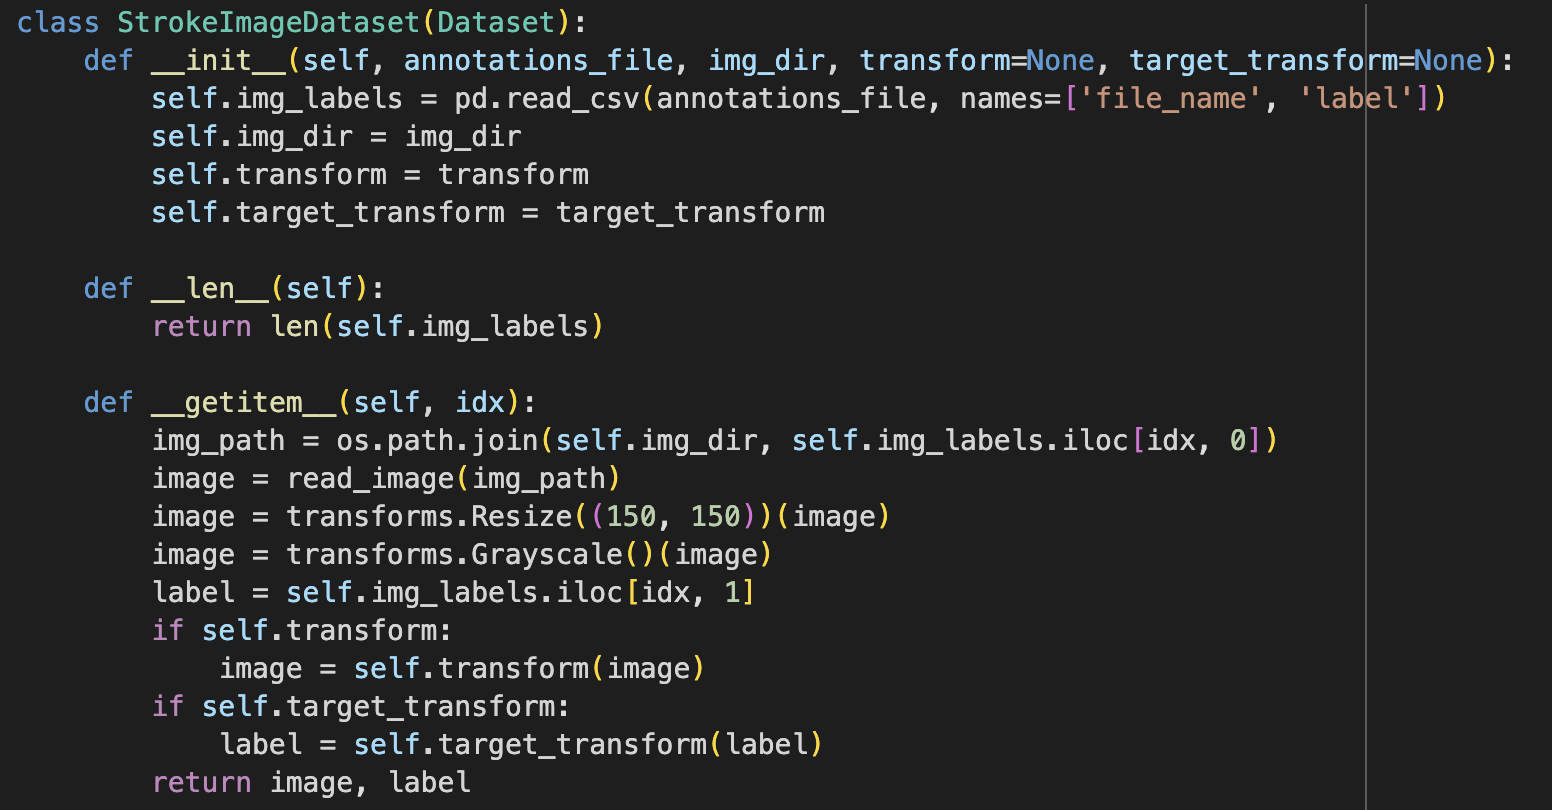
\includegraphics[width=8.5cm]{images/ViT_dataset.png}
    \caption{Dataset and Dataloader for ViT}
    \label{fig:enter-label}
\end{figure}

% 가장 중요한 MSA 모듈에 대해 상세한 구현은 다음과 같다. head 개수만큼 Q, K, V matrix를 pytorch의 Linear로 선언해서 back propagation으로 학습이 가능하도록 한다. 그리고 미리 주어진 입력에 대해 정해진 Q, K, V 내적을 진행해서 결과를 만들어낸다. 이 결과는 stack 형식으로 쌓여 있다가 모든 연산이 종료되면 입력과 동일한 차원으로 합병되어 출력한다. 즉, 연산 과정에는 head 개수만큼 분할되어 연산이 병렬적으로 진행된다. 
The detailed implementation of the most important MSA modules is as follows. Declare Q, K, and V matrices as Linear in pytorch as many as the number of heads to enable learning through back propagation. Then, the Q, K, and V dot products are performed on pre-given inputs to produce a result. These results are stacked in a stack format, and when all operations are completed, they are merged into the same dimension as the input and output. In other words, during the calculation process, the division is divided by the number of heads and the calculation is carried out in parallel.

\begin{figure}[h]
    \centering
    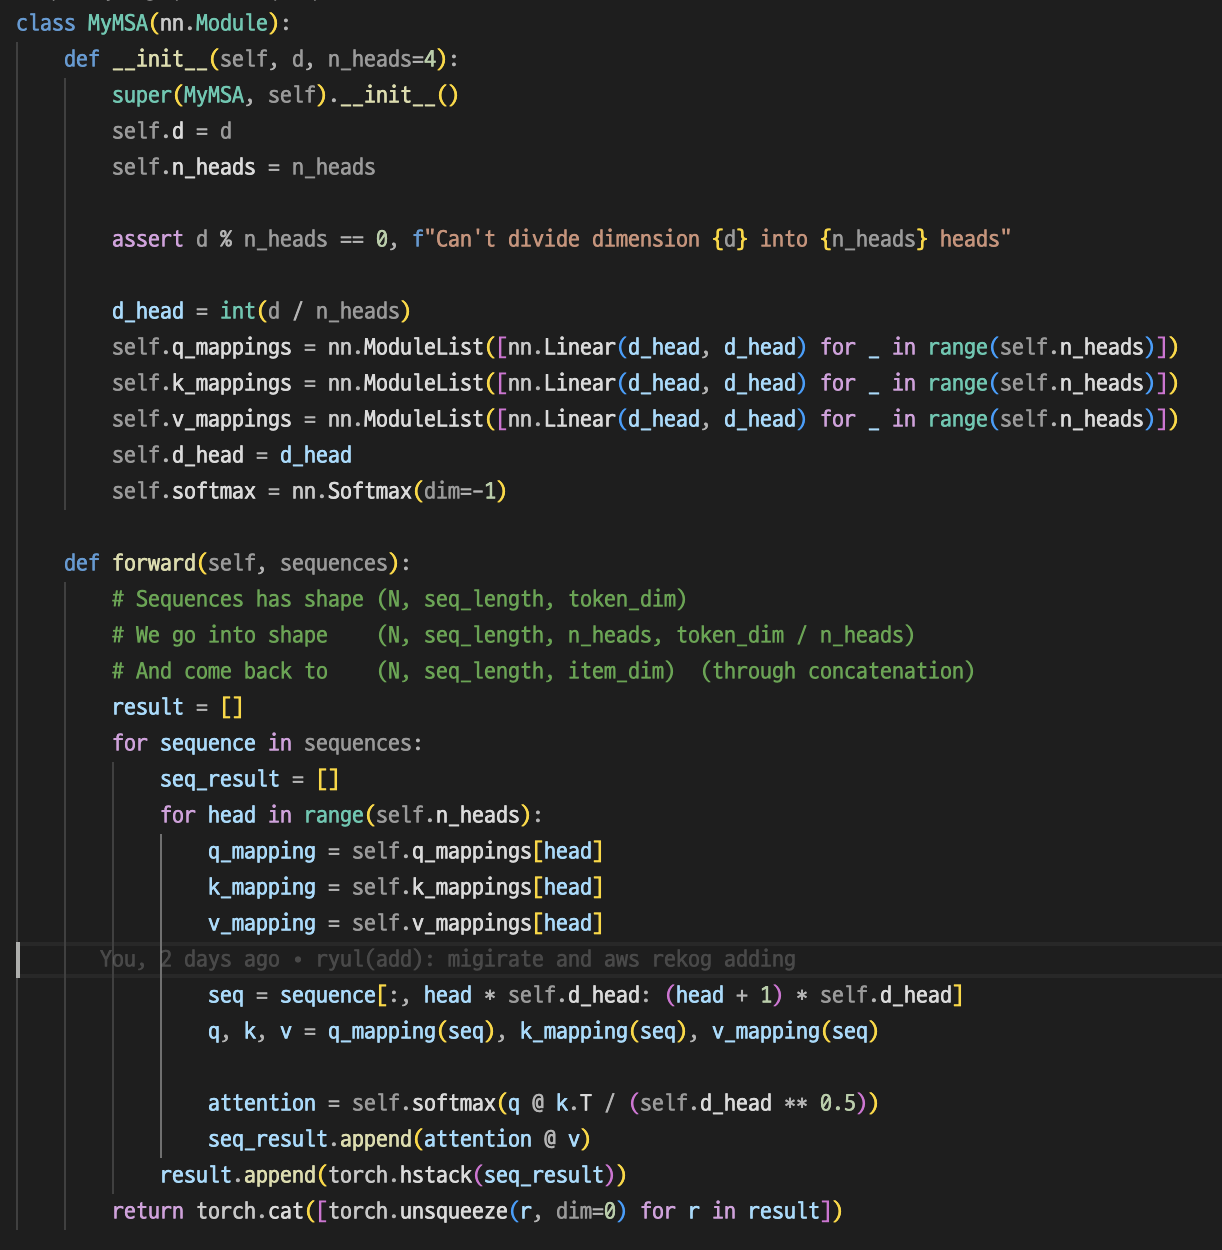
\includegraphics[width=8.5cm]{images/MyMSA.png}
    \caption{Implementation of Multi-head Self Attention}
    \label{fig:enter-label}
\end{figure}

% 위의 모듈을 만들고 아래 소스 코드와 같이 ViTBlock class를 만들어 이 class에 넣는다. 이 ViTBlock class는 MSA와 각종 결과의 정규화, Residual Connection이 포함된다.
After creating the above module, make a ViTBlock class as shown in the source code below, and insert it into this class. This ViTBlock class includes MSA, normalization of various results, and residual connection.

\begin{figure}[h]
    \centering
    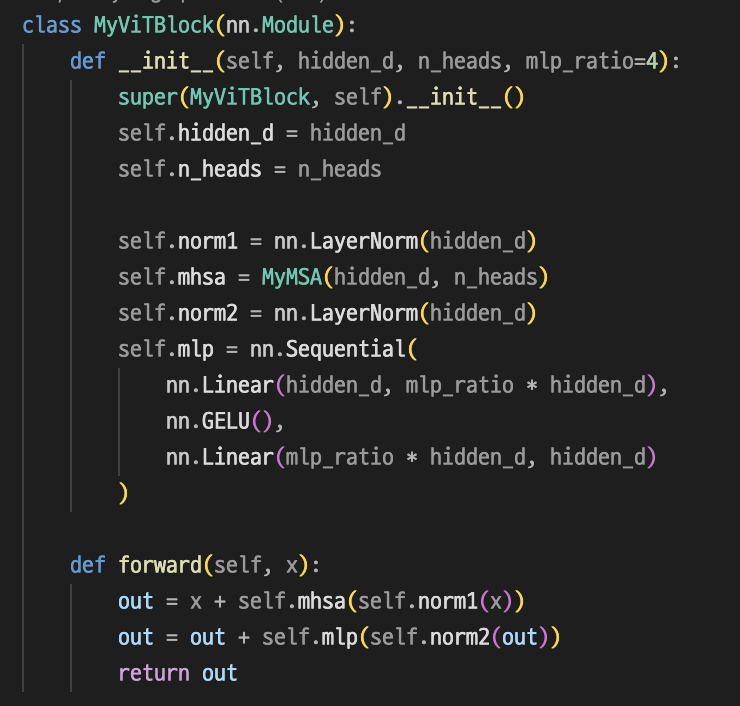
\includegraphics[width=8.5cm]{images/MyViTBlock.png}
    \caption{Implementation of ViTBlock}
    \label{fig:enter-label}
\end{figure}

% ViTBlock을 만들고 patchify, get_positional_embedding과 같은 데이터 전처리 과정을 포함해 최종적으로 아래와 같은 ViT class를 만들었다.
We created ViTBlock, including data preprocessing processes such as patchify and get\_positional\_embedding, and ultimately created the ViT class below.

\begin{figure}[h]
    \centering
    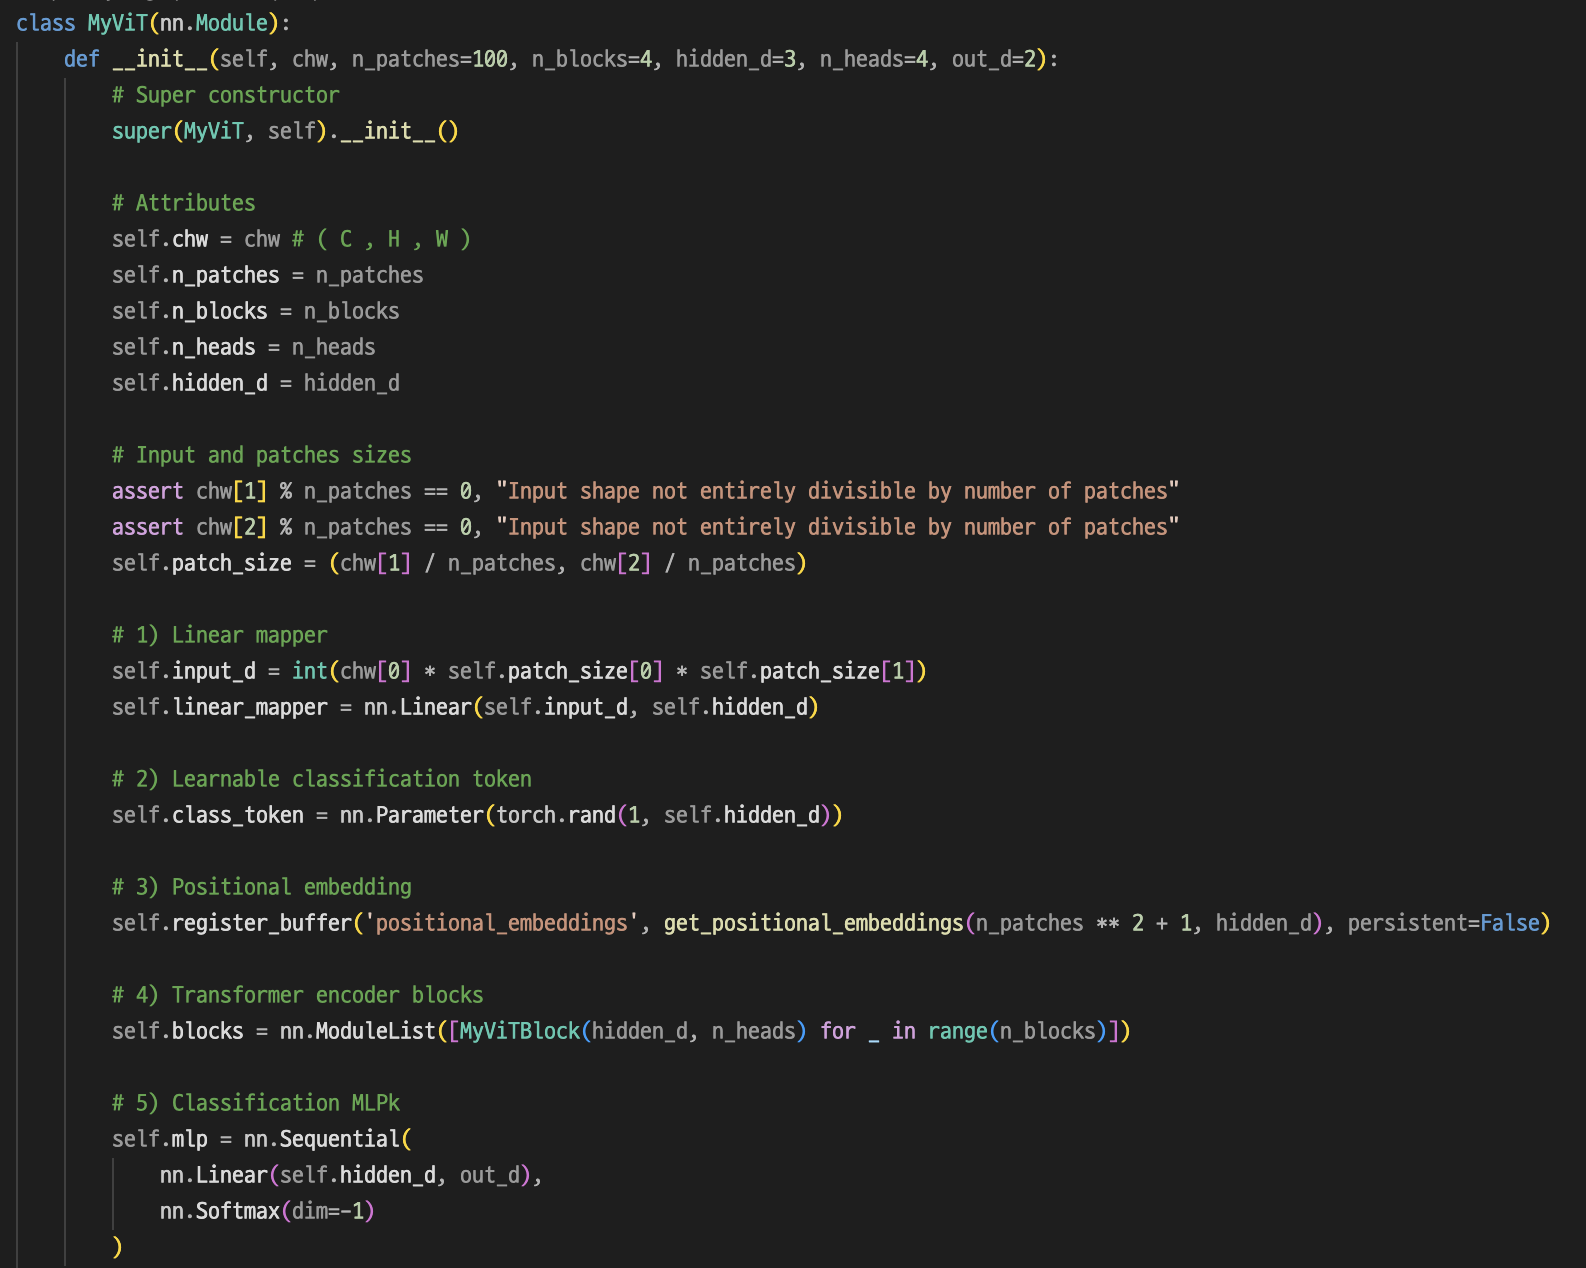
\includegraphics[width=8.5cm]{images/MyViT.png}
    \caption{Implementation of ViT class}
    \label{fig:enter-label}
\end{figure}

% 구현을 완료한 후에 main 문에서 테스트를 진행했다. Adam optimizer를 이용해서 5 epoch으로 훈련한 결과 66\% 정도의 정확도를 보였다. 수치 상으로는 제일 낮은 정확도를 보였다. 이는 학습이 충분히 이루어지지 않았다고 추론할 수 있다. ViT는 많은 데이터가 필요한데 환자의 의료 정보와 깊게 관련이 있어 충분한 양의 학습 데이터를 구하기 어려웠다. 또한 데이터가 augmented 된 데이터가 많아 중복된 데이터가 있다. ViT의 구조적인 문제와 현실의 상황 문제로 높은 성능을 나타내진 못한 것으로 생각된다.
After completing the implementation, testing was conducted in the main statement. As a result of training with 5 epochs using Adam optimizer, the accuracy was about 66\%. Numerically, it showed the lowest accuracy. This can be inferred that sufficient learning has not occurred. ViT requires a lot of data, but it is difficult to obtain a sufficient amount of learning data because it is deeply related to patients' medical information. Additionally, there is duplicated data as there is a lot of augmented data. It is believed that ViT did not achieve high performance due to structural problems and real-life situation problems.

\begin{figure}[h]
    \centering
    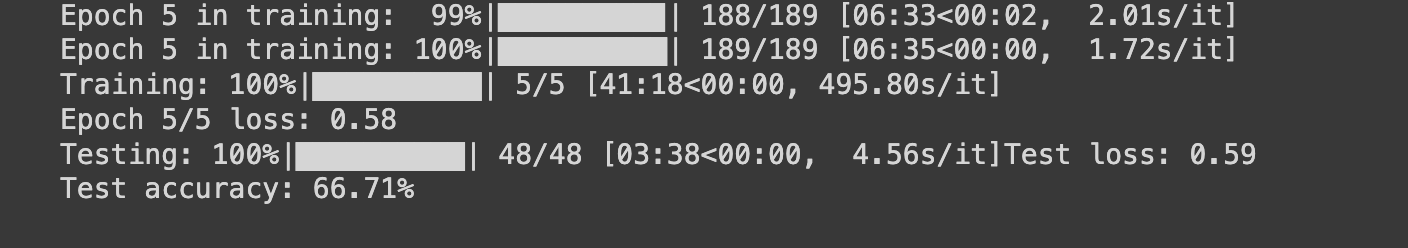
\includegraphics[width=8.5cm]{images/ViT_result.png}
    \caption{The result of testing ViT}
    \label{fig:enter-label}
\end{figure}

\textbf{se\_vitprac.py} \\
The above SE\_ViT.ipynb file was saved as a python file. The contents of the file are as above.

\begin{figure}[h]
    \centering
    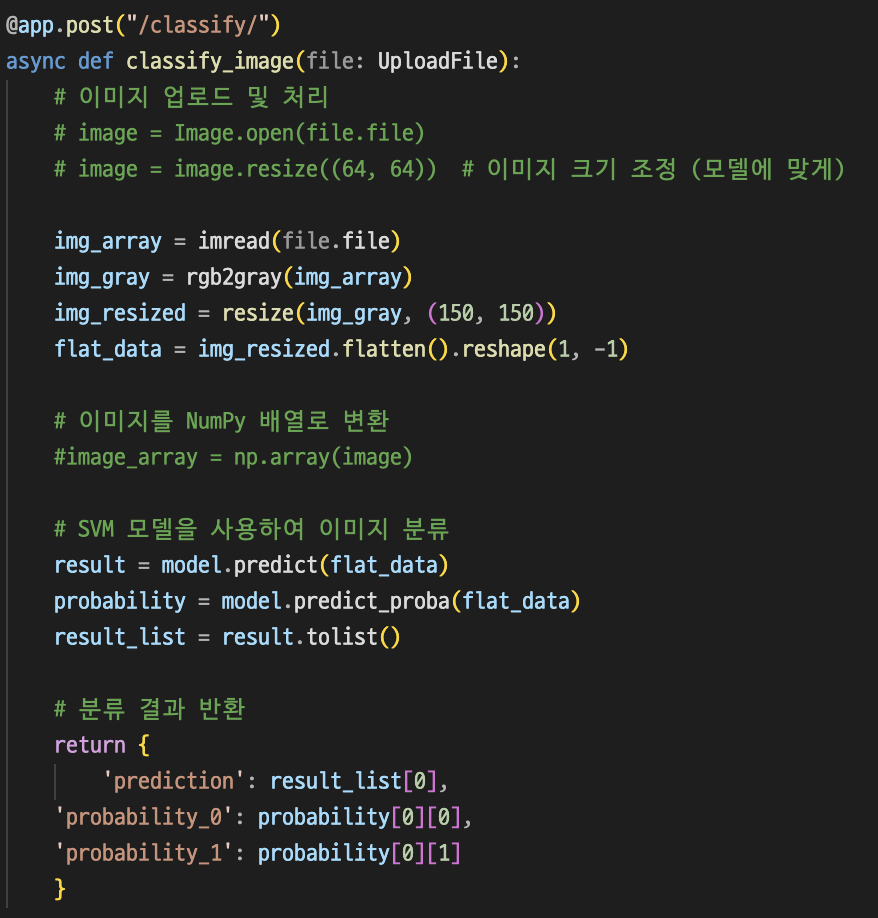
\includegraphics[width=8.5cm]{images/app.py.png}
    \caption{Core source code in app.py}
    \label{fig:enter-label}
\end{figure}

\textbf{app.py} \\
% 학습이 완료된 모델을 웹 서버로 배포하는데 사용되는 파이썬 파일이다. FastAPI와 uvicorn으로 웹 서버를 제작한다. annotation으로 @app.post("/classify/")를 붙여서 classify 형식으로 POST 요청이 왔을 때 함수가 실행되도록 만들었다. joblib 함수로 원하는 모델을 불러온다. 이미지 파일은 UploadFile의 file 변수로 받는다. 이 파일은 위 모델의 학습 과정에서 이미지 전처리 과정과 동일한 과정을 거친다. 이미지를 흑백으로 변환하고 사이즈를 통일시킨다. 그리고 벡터로 변환하고 이를 모델의 인자로 넘겨서 분류를 하도록 했다. 이때, 뇌졸중인지 아닌지 판단하고 각 상태의 확률을 함께 추론하도록 했다. 최종적으로 모델이 분류한 state와 각 state의 확률값을 json format으로 호출한 곳으로 넘겨준다. 
This is a Python file used to deploy the trained model to a web server. Build a web server with FastAPI and uvicorn. By adding @app.post("/classify/") as an annotation, I made the function run when a POST request came in classify format. Load the desired model with the joblib function. The image file is received as the file variable of UploadFile. This file goes through the same process as the image preprocessing process in the learning process of the model above. Convert the image to black and white and unify the size. Then, we converted it to a vector and passed it as a parameter to the model for classification. At this time, we were asked to determine whether it was a stroke or not and to infer the probability of each condition together. Finally, the state classified by the model and the probability value of each state are passed to the calling party in json format.


\section{\textbf{Use cases}}

\begin{figure}[H]
    \centering
    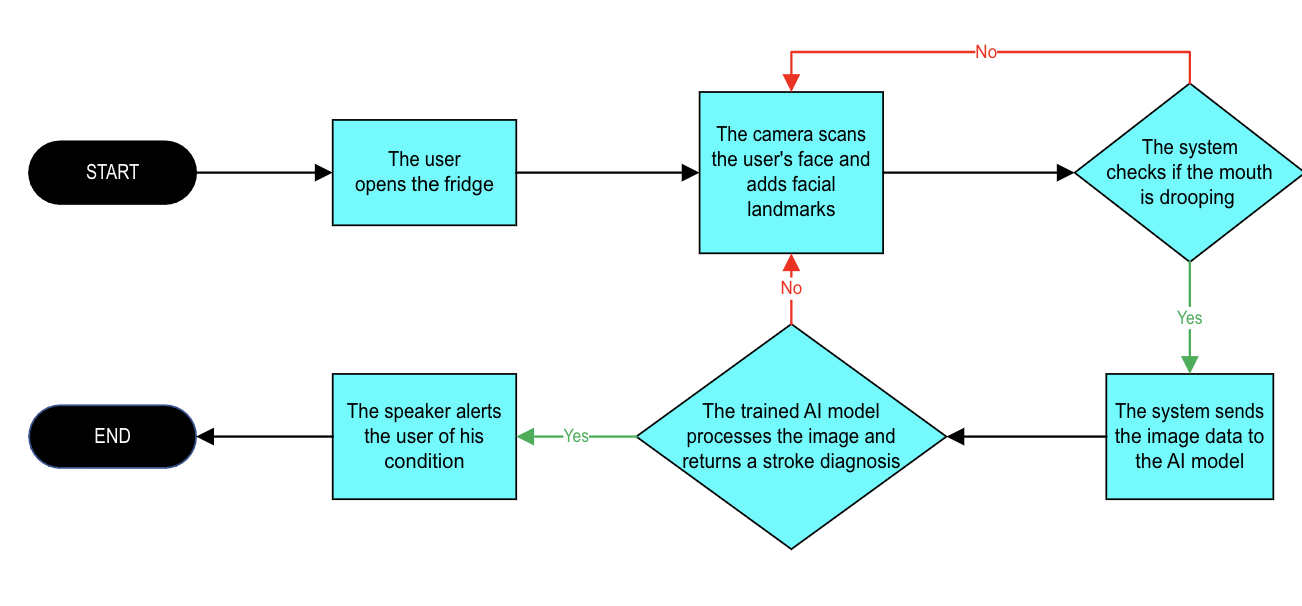
\includegraphics[width=1\linewidth]{images/use_cases.png}
    \caption{Use cases}
    \label{fig:use_cases}
\end{figure}

\subsection{\textbf{Use Case 1 : The user opens the fridge}}

\begin{figure}[H]
    \centering
    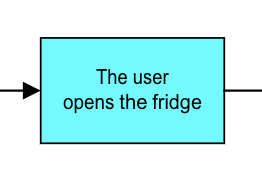
\includegraphics[width=0.33\linewidth]{images/use_case1.png}
    \caption{Use case 1}
    \label{fig:use_case1}
\end{figure}

The user goes to the refrigerator, that is equipped with a built in camera, connected to a Raspberry Pi.

\subsection{\textbf{Use Case 2 : The camera scans the user's face and adds facial landmarks}}

\begin{figure}[H]
    \centering
    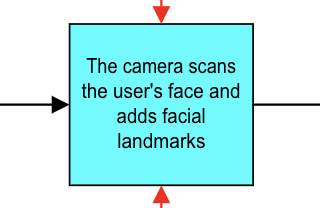
\includegraphics[width=0.33\linewidth]{images/use_case2.png}
    \caption{Use case 2}
    \label{fig:use_case2}
\end{figure}

\begin{figure}[H]
    \centering
    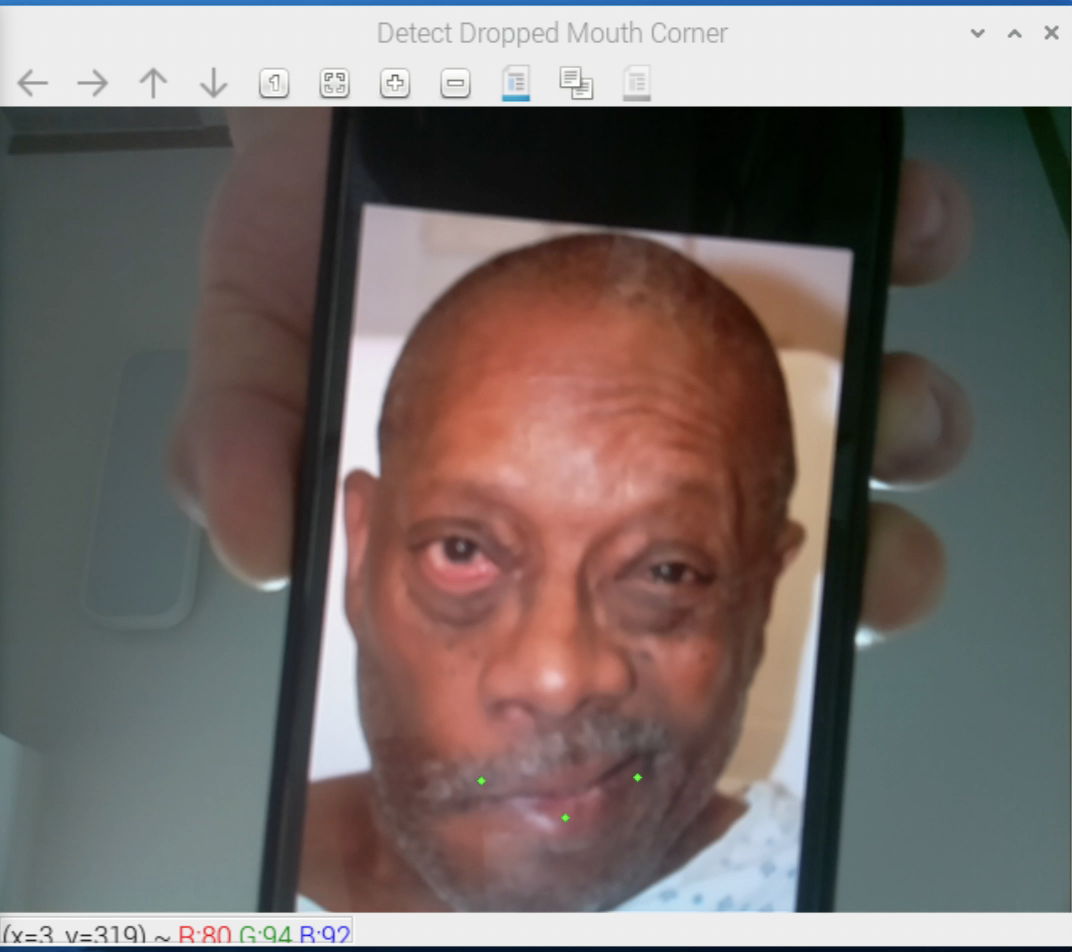
\includegraphics[width=0.5\linewidth]{images/Image.png}
    \caption{Image and facial landmarks}
    \label{fig:image and facial landmarks}
\end{figure}

This is the first level detection. The camera checks for mouth drooping in real time as long as the refrigerator is still open. The process runs offline on the local device for privacy concerns. 

\subsection{\textbf{Use Case 3 : The system checks if the mouth is drooping}}

\begin{figure}[H]
    \centering
    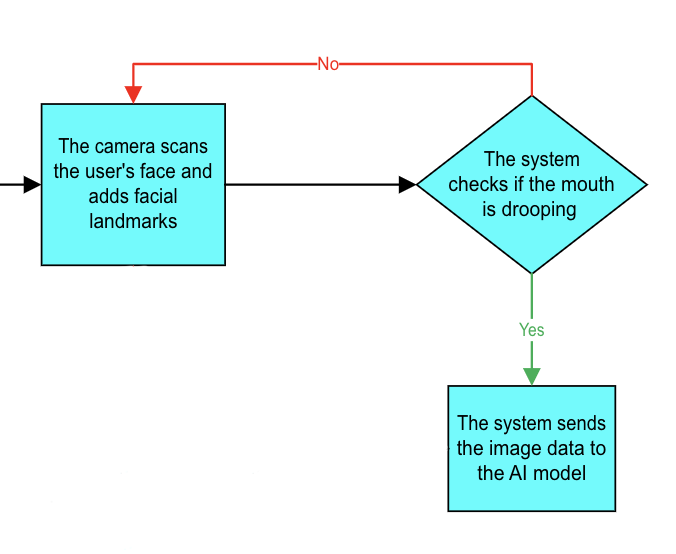
\includegraphics[width=0.7\linewidth]{images/use_case3.png}
    \caption{Use case 3}
    \label{fig:use_case3}
\end{figure}

\begin{figure}[H]
    \centering
    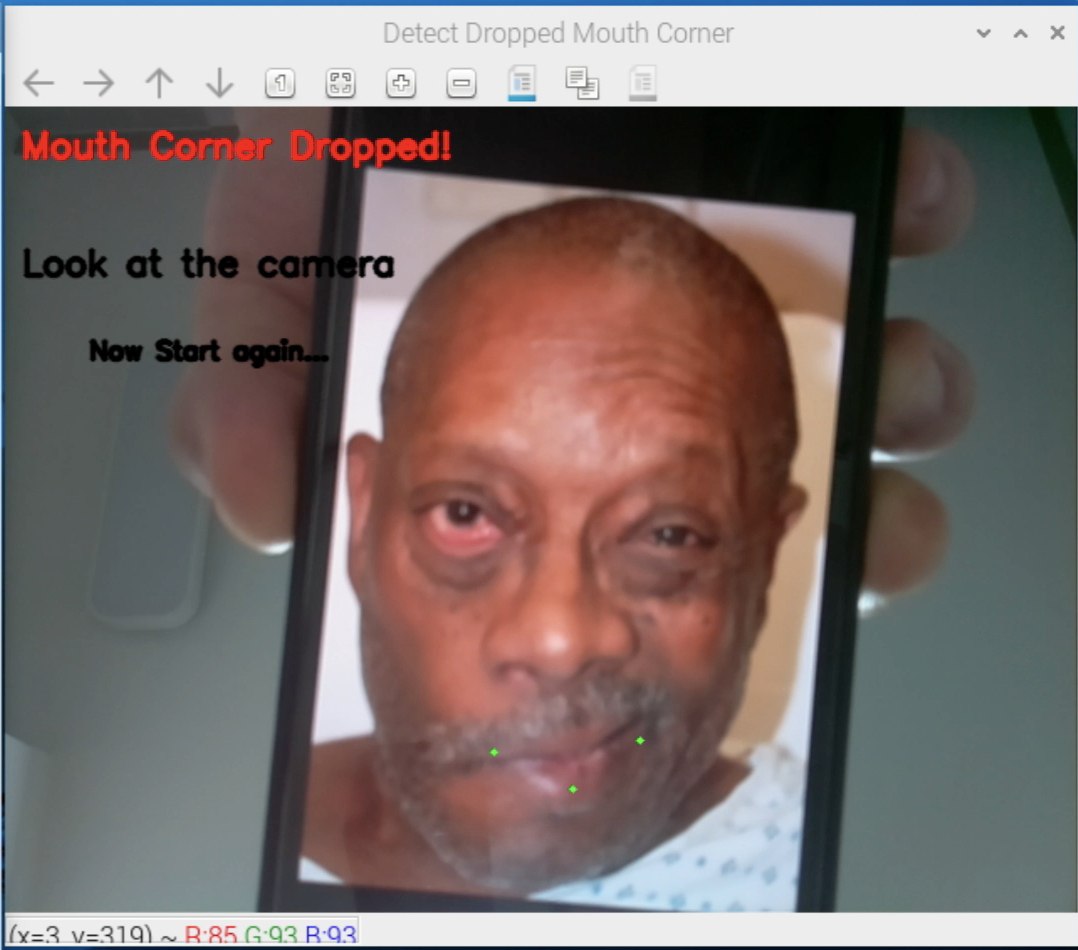
\includegraphics[width=0.5\linewidth]{images/Drooping detected.png}
    \caption{Mouth drooping}
    \label{fig:mouth drooping}
\end{figure}

\begin{figure}[H]
    \centering
    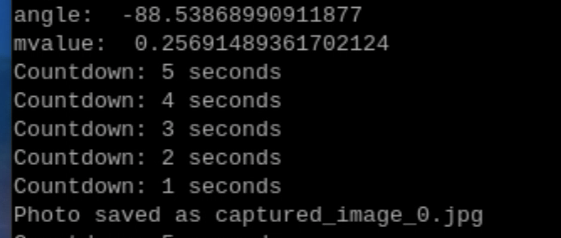
\includegraphics[width=0.7\linewidth]{images/Take picture.png}
    \caption{Picture taken}
    \label{fig:picture taken}
\end{figure}

When the camera detects the facial landmarks of the user's face, it calculates the m-value which is a value that correlate a renown symptom of stroke. If the m-value is under 0.25, nothing happens and the images taken aren't saved. However, when the m-value goes above 0.25, a more accurate picture is taken and the image data is sent to the AI model for processing.

\subsection{\textbf{Use Case 4 : The system sends the image data to the AI model}}

\begin{figure}[H]
    \centering
    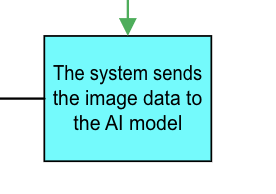
\includegraphics[width=0.33\linewidth]{images/use_case4.png}
    \caption{Use case 4}
    \label{fig:use_case4}
\end{figure}

Since the accuracy of the first level detection is low, we move to the second level detection. When the first level detection is triggered, the system establishes a connection with the server to send the image for further detection by a trained artificial intelligence model.

\subsection{\textbf{Use Case 5 : The trained AI model processes the image and return a stroke diagnosis}}

\begin{figure}[H]
    \centering
    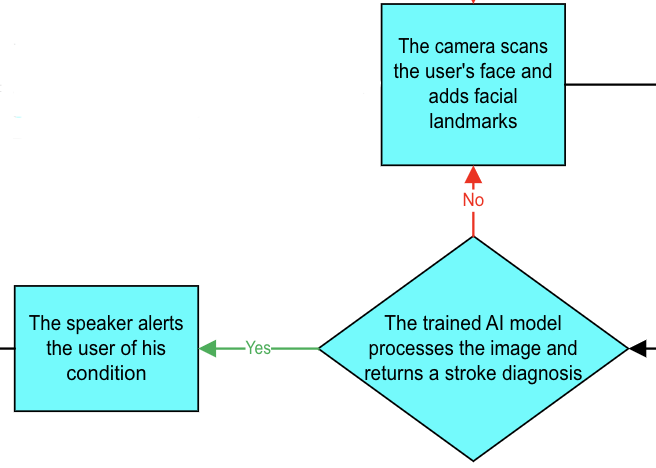
\includegraphics[width=0.7\linewidth]{images/use_case5.png}
    \caption{Use case 5}
    \label{fig:use_case5}
\end{figure}

\begin{figure}[H]
    \centering
    
\includegraphics[width=1\linewidth]{images/Result.png}
    \caption{Result}
    \label{fig:result}
\end{figure}

The image received from the Raspberry Pi is verified by the AI model. The return value is 1 for a positive stroke prognostic and 0 for a negative stroke prognostic; the probability of each value is returned also.

\subsection{\textbf{Use Case 6 : The speaker alerts the user of his condition}}

\begin{figure}[H]
    \centering
    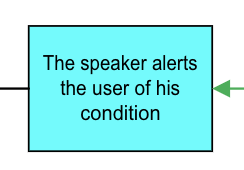
\includegraphics[width=0.33\linewidth]{images/use_case6.png}
    \caption{Use case 6}
    \label{fig:use_case6}
\end{figure}

If the diagnosis indicates the absence of a stroke, the system continues its operation with specific signals (there is no stroke symtoms). However, if the diagnosis indicates a high possibility of a stroke, the user is promptly informed of his condition through voice and a step-by-step series of actions to do is given as advice to the user in order to stay safe.

%\section{\textbf{Discussion}}

One notable difficulty encountered was in managing communication within a diverse and geographically dispersed team. As a part of a collaborative project involving team members from different cultural backgrounds, coordinating efforts and maintaining effective communication became a significant challenge. 

To overcome these challenges, the team implemented strategies such as establishing clear communication protocols, utilizing collaborative online platforms for real-time updates, and encouraging team members to provide feedback on the communication processes. Despite the initial difficulties, these measures helped enhance overall team cohesion and productivity.

This teaches the importance of proactive communication and strategic planning to address both technical and non-technical issues in a collaborative work environment.

Also, since we wanted to implement IoT technology using Raspberry Pi, we faced a lot of difficulties due to unfamiliarity with the hardware. In addition to setting up the development environment, we tried to overcome the hardware limitations by using multithreading.

Also, when using various Amazon services for MLops, we had difficulties in preprocessing the data and using the model properly. We tried to overcome this by referring to Amazon's official documentation. As a result, we realized that the dataset and preprocessing for AI are more important than the model.

% \section{Ease of Use}

% \subsection{Maintaining the Integrity of the Specifications}

% The IEEEtran class file is used to format your paper and style the text. All margins, 
% column widths, line spaces, and text fonts are prescribed; please do not 
% alter them. You may note peculiarities. For example, the head margin
% measures proportionately more than is customary. This measurement 
% and others are deliberate, using specifications that anticipate your paper 
% as one part of the entire proceedings, and not as an independent document. 
% Please do not revise any of the current designations.

% \section{Prepare Your Paper Before Styling}
% Before you begin to format your paper, first write and save the content as a 
% separate text file. Complete all content and organizational editing before 
% formatting. Please note sections \ref{AA}--\ref{SCM} below for more information on 
% proofreading, spelling and grammar.

% Keep your text and graphic files separate until after the text has been 
% formatted and styled. Do not number text heads---{\LaTeX} will do that 
% for you.

% \subsection{Abbreviations and Acronyms}\label{AA}
% Define abbreviations and acronyms the first time they are used in the text, 
% even after they have been defined in the abstract. Abbreviations such as 
% IEEE, SI, MKS, CGS, ac, dc, and rms do not have to be defined. Do not use 
% abbreviations in the title or heads unless they are unavoidable.

% \subsection{Units}
% \begin{itemize}
% \item Use either SI (MKS) or CGS as primary units. (SI units are encouraged.) English units may be used as secondary units (in parentheses). An exception would be the use of English units as identifiers in trade, such as ``3.5-inch disk drive''.
% \item Avoid combining SI and CGS units, such as current in amperes and magnetic field in oersteds. This often leads to confusion because equations do not balance dimensionally. If you must use mixed units, clearly state the units for each quantity that you use in an equation.
% \item Do not mix complete spellings and abbreviations of units: ``Wb/m\textsuperscript{2}'' or ``webers per square meter'', not ``webers/m\textsuperscript{2}''. Spell out units when they appear in text: ``. . . a few henries'', not ``. . . a few H''.
% \item Use a zero before decimal points: ``0.25'', not ``.25''. Use ``cm\textsuperscript{3}'', not ``cc''.)
% \end{itemize}

% \subsection{Equations}
% Number equations consecutively. To make your 
% equations more compact, you may use the solidus (~/~), the exp function, or 
% appropriate exponents. Italicize Roman symbols for quantities and variables, 
% but not Greek symbols. Use a long dash rather than a hyphen for a minus 
% sign. Punctuate equations with commas or periods when they are part of a 
% sentence, as in:
% \begin{equation}
% a+b=\gamma\label{eq}
% \end{equation}

% Be sure that the 
% symbols in your equation have been defined before or immediately following 
% the equation. Use ``\eqref{eq}'', not ``Eq.~\eqref{eq}'' or ``equation \eqref{eq}'', except at 
% the beginning of a sentence: ``Equation \eqref{eq} is . . .''

% \subsection{\LaTeX-Specific Advice}

% Please use ``soft'' (e.g., \verb|\eqref{Eq}|) cross references instead
% of ``hard'' references (e.g., \verb|(1)|). That will make it possible
% to combine sections, add equations, or change the order of figures or
% citations without having to go through the file line by line.

% Please don't use the \verb|{eqnarray}| equation environment. Use
% \verb|{align}| or \verb|{IEEEeqnarray}| instead. The \verb|{eqnarray}|
% environment leaves unsightly spaces around relation symbols.

% Please note that the \verb|{subequations}| environment in {\LaTeX}
% will increment the main equation counter even when there are no
% equation numbers displayed. If you forget that, you might write an
% article in which the equation numbers skip from (17) to (20), causing
% the copy editors to wonder if you've discovered a new method of
% counting.

% {\BibTeX} does not work by magic. It doesn't get the bibliographic
% data from thin air but from .bib files. If you use {\BibTeX} to produce a
% bibliography you must send the .bib files. 

% {\LaTeX} can't read your mind. If you assign the same label to a
% subsubsection and a table, you might find that Table I has been cross
% referenced as Table IV-B3. 

% {\LaTeX} does not have precognitive abilities. If you put a
% \verb|\label| command before the command that updates the counter it's
% supposed to be using, the label will pick up the last counter to be
% cross referenced instead. In particular, a \verb|\label| command
% should not go before the caption of a figure or a table.

% Do not use \verb|\nonumber| inside the \verb|{array}| environment. It
% will not stop equation numbers inside \verb|{array}| (there won't be
% any anyway) and it might stop a wanted equation number in the
% surrounding equation.

% \subsection{Some Common Mistakes}\label{SCM}
% \begin{itemize}
% \item The word ``data'' is plural, not singular.
% \item The subscript for the permeability of vacuum $\mu_{0}$, and other common scientific constants, is zero with subscript formatting, not a lowercase letter ``o''.
% \item In American English, commas, semicolons, periods, question and exclamation marks are located within quotation marks only when a complete thought or name is cited, such as a title or full quotation. When quotation marks are used, instead of a bold or italic typeface, to highlight a word or phrase, punctuation should appear outside of the quotation marks. A parenthetical phrase or statement at the end of a sentence is punctuated outside of the closing parenthesis (like this). (A parenthetical sentence is punctuated within the parentheses.)
% \item A graph within a graph is an ``inset'', not an ``insert''. The word alternatively is preferred to the word ``alternately'' (unless you really mean something that alternates).
% \item Do not use the word ``essentially'' to mean ``approximately'' or ``effectively''.
% \item In your paper title, if the words ``that uses'' can accurately replace the word ``using'', capitalize the ``u''; if not, keep using lower-cased.
% \item Be aware of the different meanings of the homophones ``affect'' and ``effect'', ``complement'' and ``compliment'', ``discreet'' and ``discrete'', ``principal'' and ``principle''.
% \item Do not confuse ``imply'' and ``infer''.
% \item The prefix ``non'' is not a word; it should be joined to the word it modifies, usually without a hyphen.
% \item There is no period after the ``et'' in the Latin abbreviation ``et al.''.
% \item The abbreviation ``i.e.'' means ``that is'', and the abbreviation ``e.g.'' means ``for example''.
% \end{itemize}
% An excellent style manual for science writers is \cite{b7}.

% \subsection{Authors and Affiliations}
% \textbf{The class file is designed for, but not limited to, six authors.} A 
% minimum of one author is required for all conference articles. Author names 
% should be listed starting from left to right and then moving down to the 
% next line. This is the author sequence that will be used in future citations 
% and by indexing services. Names should not be listed in columns nor group by 
% affiliation. Please keep your affiliations as succinct as possible (for 
% example, do not differentiate among departments of the same organization).

% \subsection{Identify the Headings}
% Headings, or heads, are organizational devices that guide the reader through 
% your paper. There are two types: component heads and text heads.

% Component heads identify the different components of your paper and are not 
% topically subordinate to each other. Examples include Acknowledgments and 
% References and, for these, the correct style to use is ``Heading 5''. Use 
% ``figure caption'' for your Figure captions, and ``table head'' for your 
% table title. Run-in heads, such as ``Abstract'', will require you to apply a 
% style (in this case, italic) in addition to the style provided by the drop 
% down menu to differentiate the head from the text.

% Text heads organize the topics on a relational, hierarchical basis. For 
% example, the paper title is the primary text head because all subsequent 
% material relates and elaborates on this one topic. If there are two or more 
% sub-topics, the next level head (uppercase Roman numerals) should be used 
% and, conversely, if there are not at least two sub-topics, then no subheads 
% should be introduced.

% \subsection{Figures and Tables}
% \paragraph{Positioning Figures and Tables} Place figures and tables at the top and 
% bottom of columns. Avoid placing them in the middle of columns. Large 
% figures and tables may span across both columns. Figure captions should be 
% below the figures; table heads should appear above the tables. Insert 
% figures and tables after they are cited in the text. Use the abbreviation 
% ``Fig.~\ref{fig}'', even at the beginning of a sentence.

% \begin{table}[htbp]
% \caption{Table Type Styles}
% \begin{center}
% \begin{tabular}{|c|c|c|c|}
% \hline
% \textbf{Table}&\multicolumn{3}{|c|}{\textbf{Table Column Head}} \\
% \cline{2-4} 
% \textbf{Head} & \textbf{\textit{Table column subhead}}& \textbf{\textit{Subhead}}& \textbf{\textit{Subhead}} \\
% \hline
% copy& More table copy$^{\mathrm{a}}$& &  \\
% \hline
% \multicolumn{4}{l}{$^{\mathrm{a}}$Sample of a Table footnote.}
% \end{tabular}
% \label{tab1}
% \end{center}
% \end{table}

% \begin{figure}[htbp]
% \centerline{\includegraphics{}}
% \caption{Example of a figure caption.}
% \label{fig}
% \end{figure}

% Figure Labels: Use 8 point Times New Roman for Figure labels. Use words 
% rather than symbols or abbreviations when writing Figure axis labels to 
% avoid confusing the reader. As an example, write the quantity 
% ``Magnetization'', or ``Magnetization, M'', not just ``M''. If including 
% units in the label, present them within parentheses. Do not label axes only 
% with units. In the example, write ``Magnetization (A/m)'' or ``Magnetization 
% \{A[m(1)]\}'', not just ``A/m''. Do not label axes with a ratio of 
% quantities and units. For example, write ``Temperature (K)'', not 
% ``Temperature/K''.

% \section*{Acknowledgment}

% The preferred spelling of the word ``acknowledgment'' in America is without 
% an ``e'' after the ``g''. Avoid the stilted expression ``one of us (R. B. 
% G.) thanks $\ldots$''. Instead, try ``R. B. G. thanks$\ldots$''. Put sponsor 
% acknowledgments in the unnumbered footnote on the first page.

% \section*{References}

% Please number citations consecutively within brackets \cite{b1}. The 
% sentence punctuation follows the bracket \cite{b2}. Refer simply to the reference 
% number, as in \cite{b3}---do not use ``Ref. \cite{b3}'' or ``reference \cite{b3}'' except at 
% the beginning of a sentence: ``Reference \cite{b3} was the first $\ldots$''

% Number footnotes separately in superscripts. Place the actual footnote at 
% the bottom of the column in which it was cited. Do not put footnotes in the 
% abstract or reference list. Use letters for table footnotes.

% Unless there are six authors or more give all authors' names; do not use 
% ``et al.''. Papers that have not been published, even if they have been 
% submitted for publication, should be cited as ``unpublished'' \cite{b4}. Papers 
% that have been accepted for publication should be cited as ``in press'' \cite{b5}. 
% Capitalize only the first word in a paper title, except for proper nouns and 
% element symbols.

% For papers published in translation journals, please give the English 
% citation first, followed by the original foreign-language citation \cite{b6}.

% \begin{thebibliography}{00}
% \bibitem{1} National Statistical Office, Cause of death statistics results, 2022

% \bibitem{2} About Stroke, American Stroke Association, http://aiweb.techfak.uni-bielefeld.de/content/bworld-robot-control-software/

% \bibitem{3} Spiotta, Alejandro M., et al. "The golden hour of stroke intervention: effect of thrombectomy procedural time in acute ischemic stroke on outcome." Journal of neurointerventional surgery 6.7 (2014): 511-516.

% \bibitem{4} 뇌졸중, 위키백과, https://ko.wikipedia.org/w/index.phptitle=%EB%87%8C%EC%A1%B8%EC%A4%91&oldid=34409902 

% \bibitem{5} El Ammar, F., Ardelt, A., Del Brutto, V. J., Loggini, A., Bulwa, Z., Martinez, R. C., ... & Goldenberg, F. D. (2020). BE-FAST: a sensitive screening tool to identify in-hospital acute ischemic stroke. Journal of stroke and cerebrovascular diseases, 29(7), 104821.

% \bibitem{6} 중앙일보, 60\% 더 비싼 ‘문안의 문’ 냉장고 불티 왜, https://www.joongang.co.kr/article/8013466#home, 2012

% \bibitem{7} ELIZABETHTOWN GAS, Cold Facts About Your Refrigerator, https://www.elizabethtowngas.com/conserve/cold-facts-about-your-refrigerator

% \bibitem{8} Leesungsu
% \end{thebibliography}
% \vspace{14pt}
% \color{red}
% IEEE conference templates contain guidance text for composing and formatting conference papers. Please ensure that all template text is removed from your conference paper prior to submission to the conference. Failure to remove the template text from your paper may result in your paper not being published.

\bibliographystyle{unsrt}
\bibliography{reference}


\end{document}